\documentclass[12pt,letterpaper]{article}

\usepackage{graphicx}
\usepackage{graphicx,textcomp}
\usepackage{setspace}
\usepackage{fullpage}
\usepackage{color}
\usepackage[reqno]{amsmath}
\usepackage{amsthm}
\usepackage{fancyvrb}
\usepackage{amssymb,enumerate}
\usepackage[all]{xy}
\usepackage{endnotes}
\usepackage{lscape}
\newtheorem{com}{Comment}
\usepackage{float}
\newtheorem{lem} {Lemma}
\newtheorem{prop}{Proposition}
\newtheorem{thm}{Theorem}
\newtheorem{defn}{Definition}
\newtheorem{cor}{Corollary}
\newtheorem{obs}{Observation}

\usepackage[compact]{titlesec}
\usepackage{dcolumn}
\usepackage{tikz}
\usetikzlibrary{arrows}
\usepackage{multirow}
\usepackage{xcolor}
\newcolumntype{.}{D{.}{.}{-1}}
\newcolumntype{d}[1]{D{.}{.}{#1}}
\definecolor{light-gray}{gray}{0.65}
\usepackage{url}
\usepackage{listings}
\usepackage{color}
\usepackage{adjustbox}
\usepackage{caption}
\captionsetup{justification=centering}

\usepackage{hyperref}
\usepackage{longtable}

%%%% BIBLIOGRAPHY SETTINGS %%%%

\usepackage[backend=biber, notes, isbn=false, doi=false, url=false]{biblatex-chicago}
\addbibresource{/Users/sarabcidf/Desktop/ASDS/Dissertation/Latex/PopulismBiblio2.bib}

\definecolor{codegreen}{rgb}{0,0.6,0}
\definecolor{codegray}{rgb}{0.5,0.5,0.5}
\definecolor{codepurple}{rgb}{0.58,0,0.82}
\definecolor{backcolour}{rgb}{0.95,0.95,0.92}

\lstdefinestyle{mystyle}{
	backgroundcolor=\color{backcolour},   
	commentstyle=\color{codegreen},
	keywordstyle=\color{magenta},
	numberstyle=\tiny\color{codegray},
	stringstyle=\color{codepurple},
	basicstyle=\footnotesize,
	breakatwhitespace=false,         
	breaklines=true,                 
	captionpos=b,                    
	keepspaces=true,                 
	numbers=left,                    
	numbersep=5pt,                  
	showspaces=false,                
	showstringspaces=false,
	showtabs=false,                  
	tabsize=2
}

% Tables %

\usepackage{multirow}
\usepackage{cellspace} % for cell margins
\setlength\cellspacetoplimit{5pt} % Adjust the top margin
\setlength\cellspacebottomlimit{5pt} % Adjust the bottom margin

%%%% SECTIONS FORMATTING %%%%

\titleformat{\section}[hang]
{\normalfont\Large\bfseries}{\thesection}{1em}{}
\titlespacing*{\section}
{0pt}{0pt plus 4pt minus 2pt}{0pt plus 2pt minus 2pt}
\newcommand{\sectionbreak}{\clearpage}

\lstset{style=mystyle}
\newcommand{\Sref}[1]{Section~\ref{#1}}
\newtheorem{hyp}{Hypothesis}

%%%% DOCUMENT %%%%

\begin{document}
	
	% Cover page
	
	\begin{titlepage}
		\centering
		\vspace*{1cm} % Add vertical space at the top of the page
		
		% Include the logo
		
\includegraphics[width=\textwidth]{Trinity_RGB_transparent_main.png}\\[1cm]
		
		% Thesis title
		{\LARGE Populism Beyond the West: A Computational Approach to Measuring Populism and an Analysis of its Dimensions in Latin America}\\[1cm]
		{\Large Online Appendix 2: Alternative Models Comparison and Full Model Evaluation Metrics}\\[0.3cm]
		
		% Supervisor
		\Large Sara Belén Cid Ferro \\[1cm]
		
		% Date
		{\large \today}
	\end{titlepage}
	
	% Contents
	
	\tableofcontents
	\listoffigures
	\listoftables
	
	\section{Metrics Comparisons for Alternative Models}
	
	\begin{table}[H]
		\centering
		\caption{Final Model Performance Metrics}
		\begin{tabular}{|c|c|c|c|}
			\hline
			\multicolumn{4}{|c|}{\textbf{Different Models by Country, BoW, RF}} \\
			\hline
			& \textbf{Lowest} & \textbf{Highest} & \textbf{Average} \\
			\hline
			Best Score & 0.19 & 3.73 & 1.98 \\
			\hline
			MSE & 0.15 & 3.82 & 1.97 \\
			\hline
		\end{tabular}
	\end{table}
	
	\begin{table}[H]
		\centering
		\caption{Single Model Comparison}
		\begin{tabular}{|c|c|}
			\hline
			\multicolumn{2}{|c|}{\textbf{Single Model}} \\
			\hline
			Best Score & 4.741 \\
			\hline
			MSE & 4.63 \\
			\hline
		\end{tabular}
	\end{table}
	
	\begin{table}[H]
		\centering
		\caption{TD-IDF Models Comparison}
		\begin{tabular}{|c|c|c|c|}
			\hline
			\multicolumn{4}{|c|}{\textbf{Different Models by Country, TD-IDF, RF}} \\
			\hline
			& \textbf{Lowest} & \textbf{Highest} & \textbf{Average} \\
			\hline
			Best Score & 0.19 & 3.78 & 2.03 \\
			\hline
			MSE & 0.14 & 3.68 & 1.94 \\
			\hline
		\end{tabular}
	\end{table}
	
	\begin{table}[H]
		\centering
		\caption{Gradient Boosting Models Comparison}
		\begin{tabular}{|c|c|c|c|}
			\hline
			\multicolumn{4}{|c|}{\textbf{Different Models by Country, BoW, GB}} \\
			\hline
			& \textbf{Lowest} & \textbf{Highest} & \textbf{Average} \\
			\hline
			Best Score & 0.18 & 3.77 & 1.95 \\
			\hline
			MSE & 0.13 & 3.72 & 1.94 \\
			\hline
		\end{tabular}
	\end{table}
	
	\begin{table}[H]
		\centering
		\caption{Extreme Gradient Boosting Models Comparison}
		\begin{tabular}{|c|c|c|c|}
			\hline
			\multicolumn{4}{|c|}{\textbf{Different Models by Country, BoW, XGB}} \\
			\hline
			& \textbf{Lowest} & \textbf{Highest} & \textbf{Average} \\
			\hline
			Best Score & 0.18 & 3.76 & 1.95 \\
			\hline
			MSE & 0.13 & 3.78 & 1.93 \\
			\hline
		\end{tabular}
	\end{table}
	
	\newpage
	\section{Performance and Validation Metrics for the Selected Model}
	
	\subsection{Bolivia}
	\begin{figure}[H]
		\centering
		\caption{Feature Importance for Bolivia Model}
		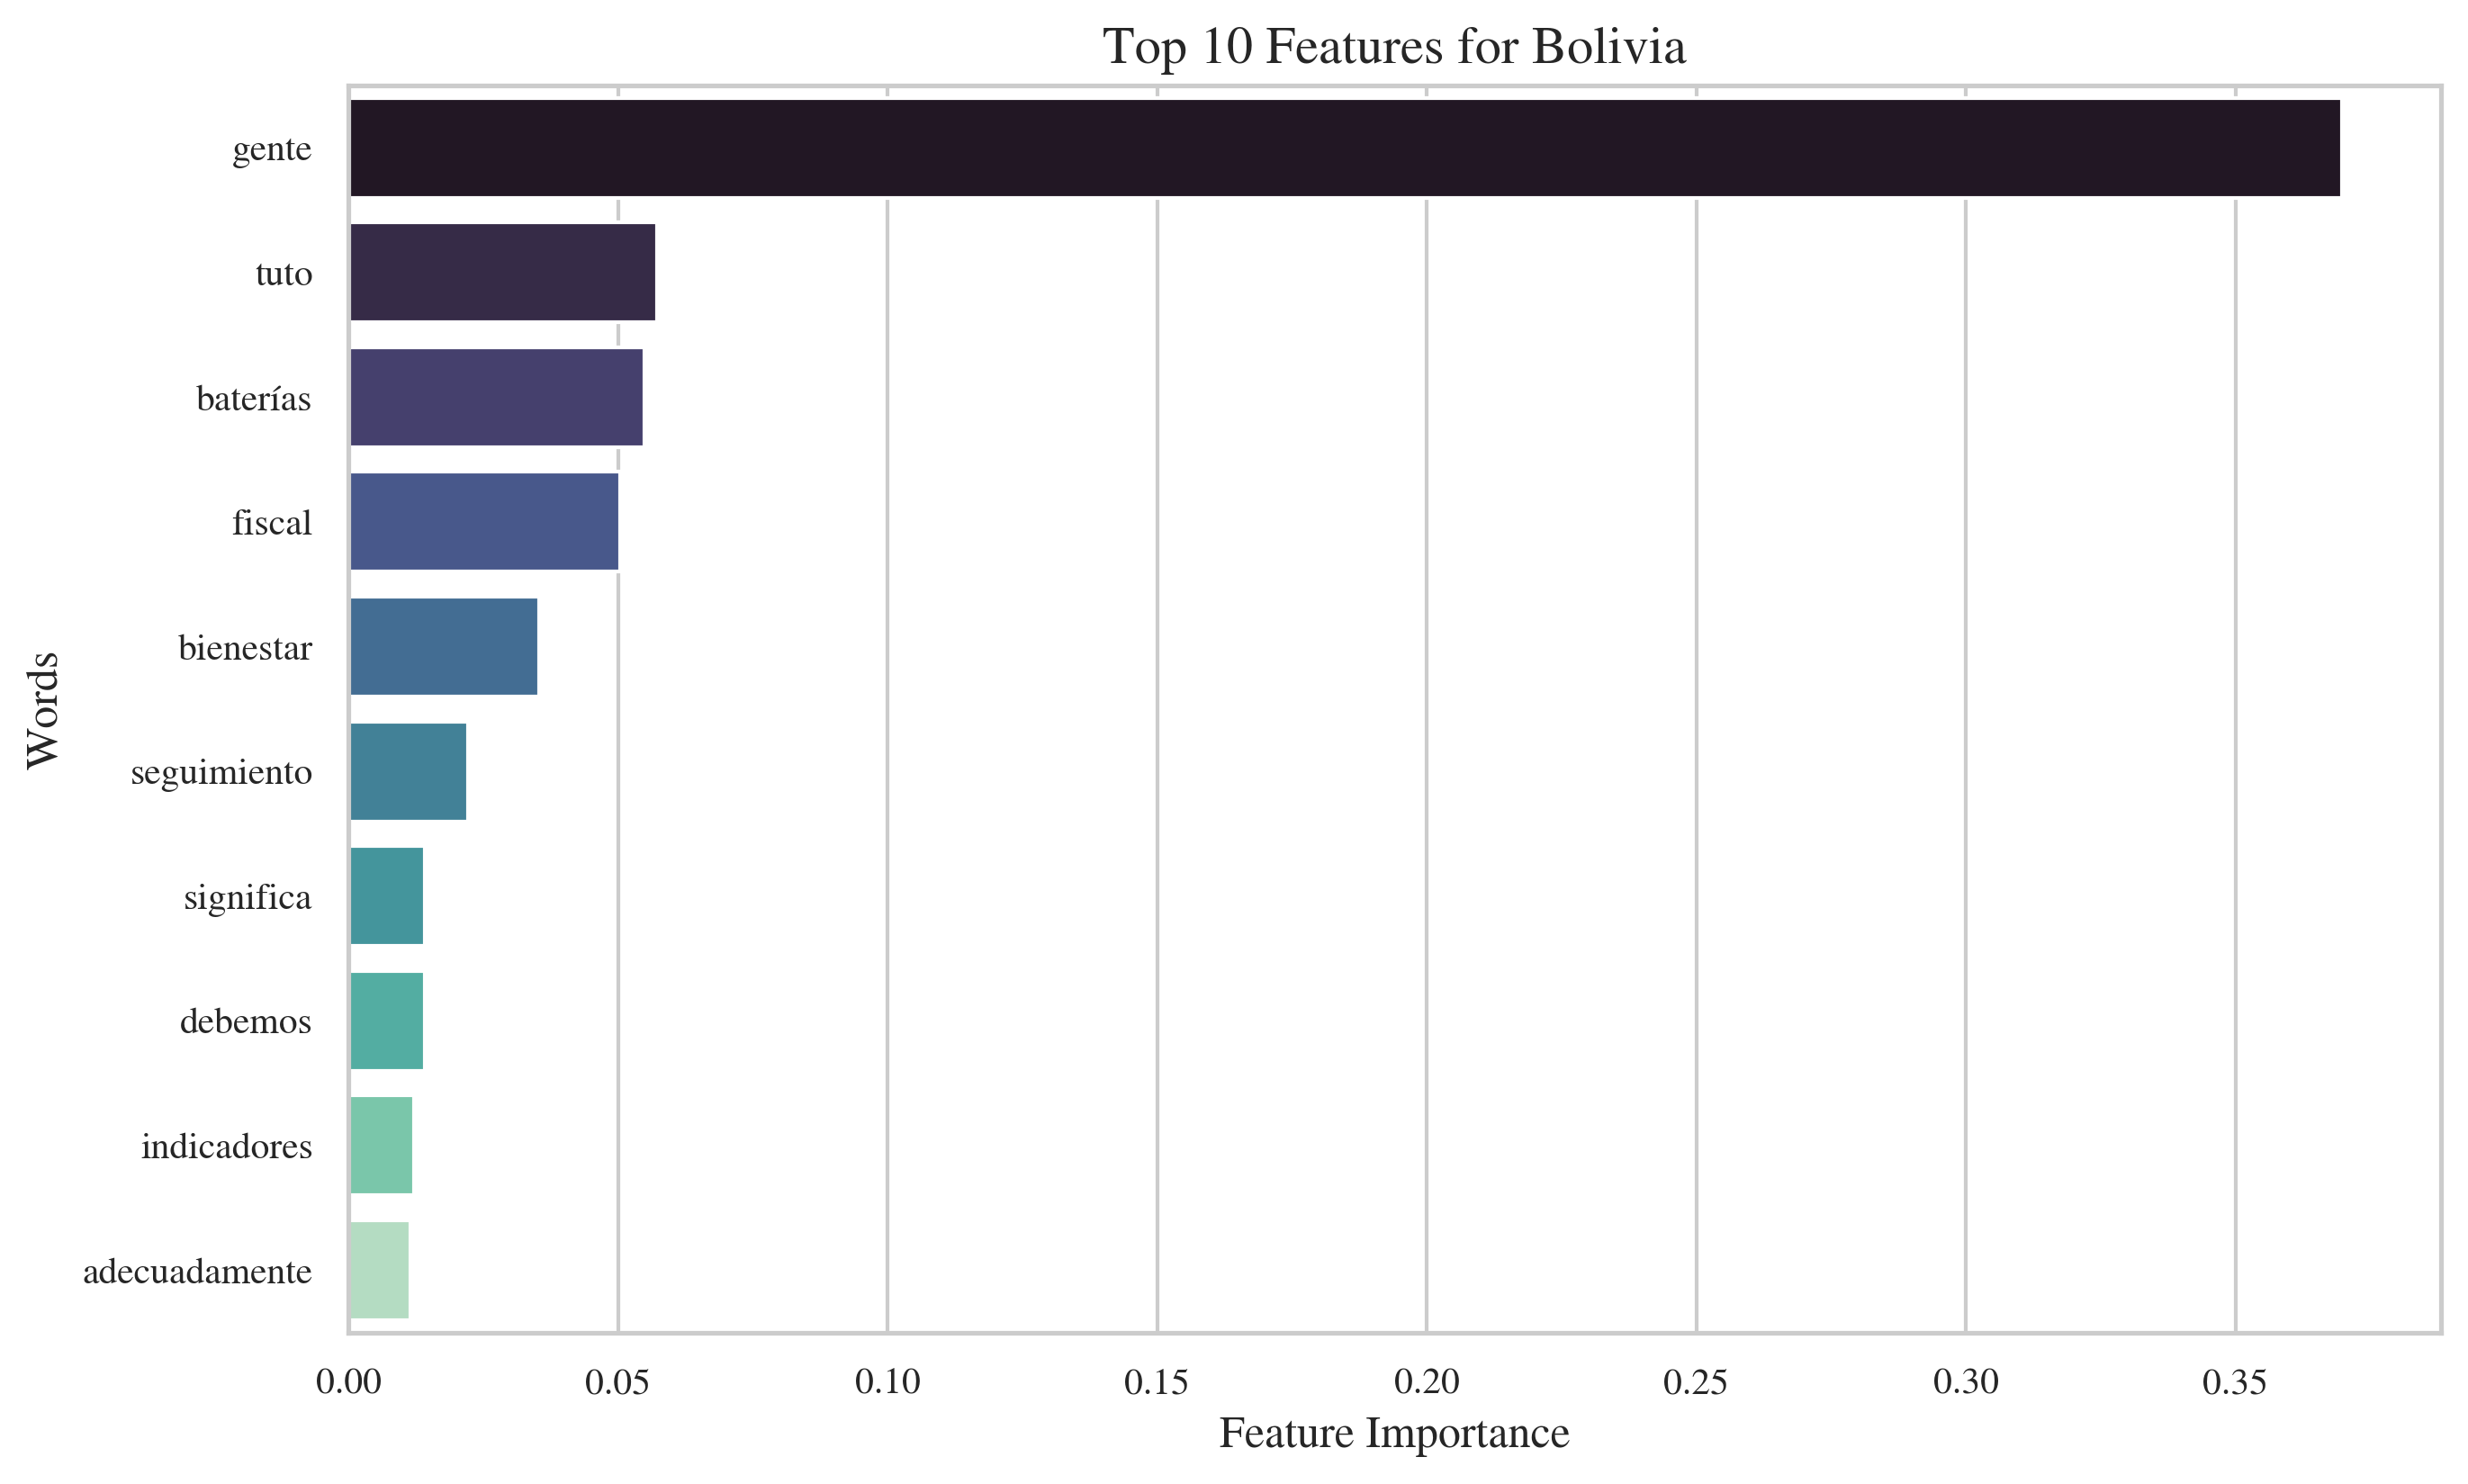
\includegraphics[width=0.8\textwidth]{/Users/sarabcidf/Desktop/ASDS/Dissertation/FinalScripts/CallanByCountry/Bolivia_feature_importance.png}
	\end{figure}
	\begin{figure}[H]
		\centering
		\caption{Error Rate for Bolivia Model}
		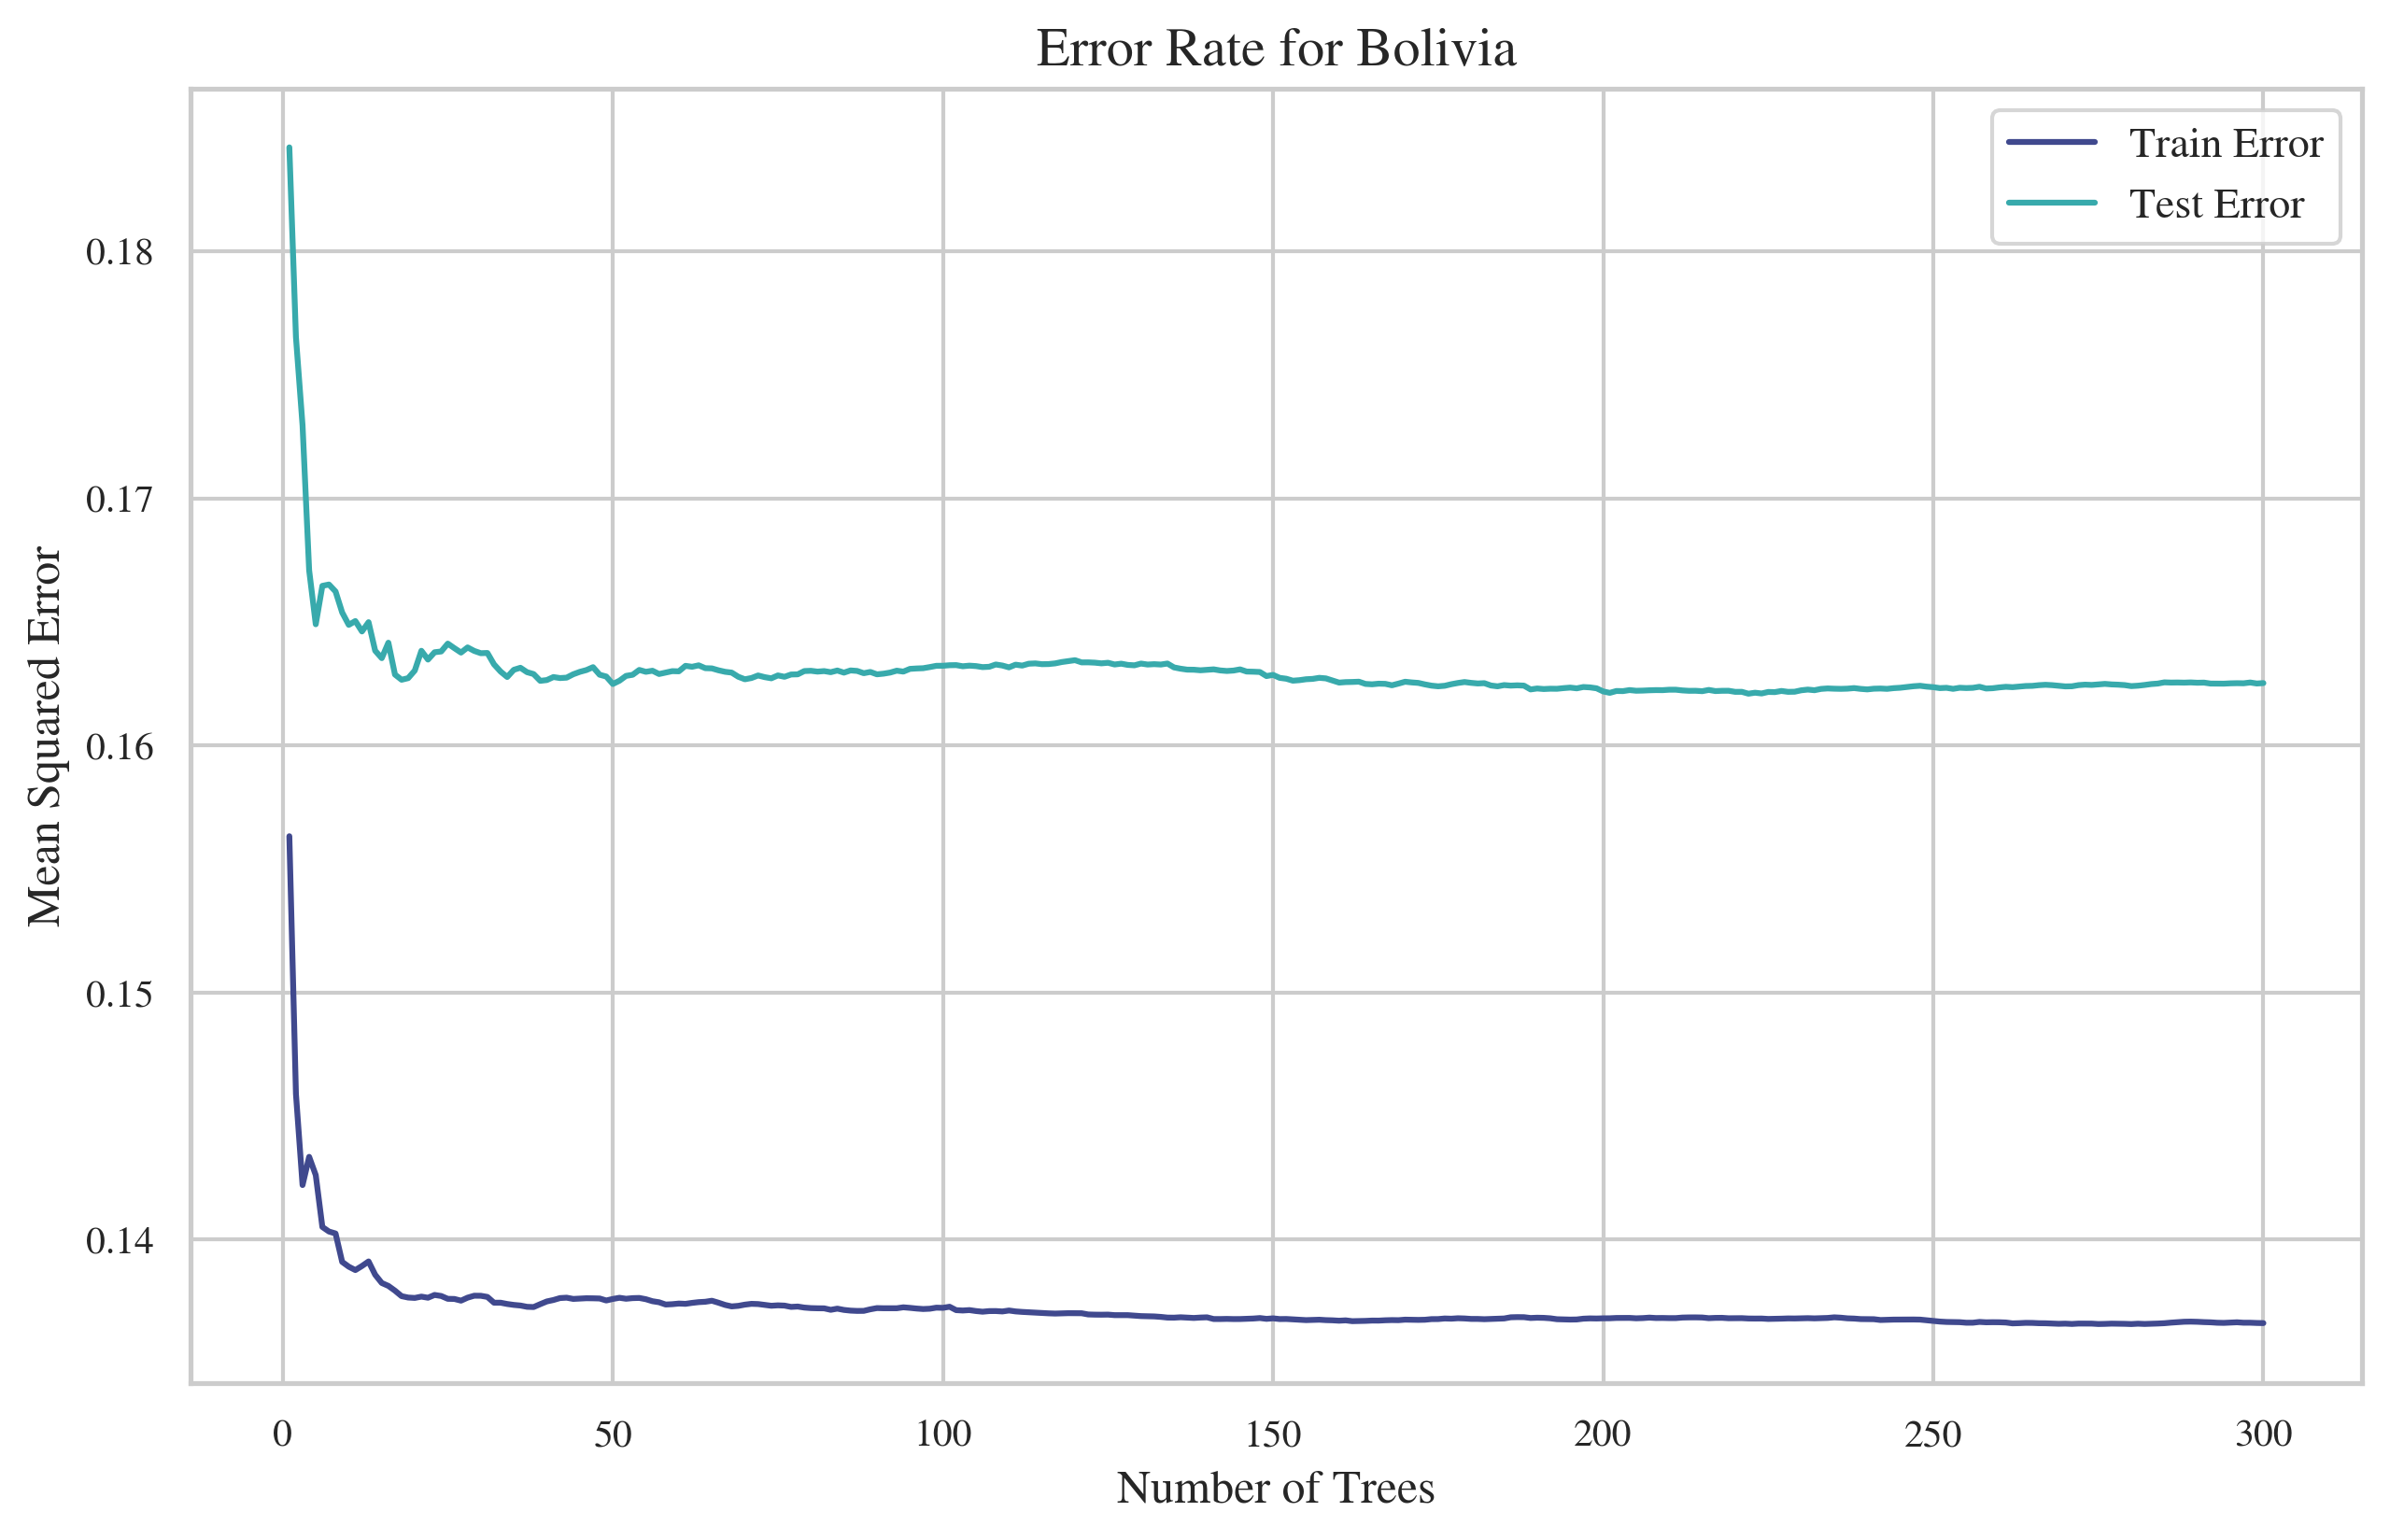
\includegraphics[width=0.8\textwidth]{/Users/sarabcidf/Desktop/ASDS/Dissertation/FinalScripts/CallanByCountry/Bolivia_error_rate.png}
	\end{figure}
	\begin{figure}[H]
		\centering
		\caption{Learning Curve for Bolivia Model}
		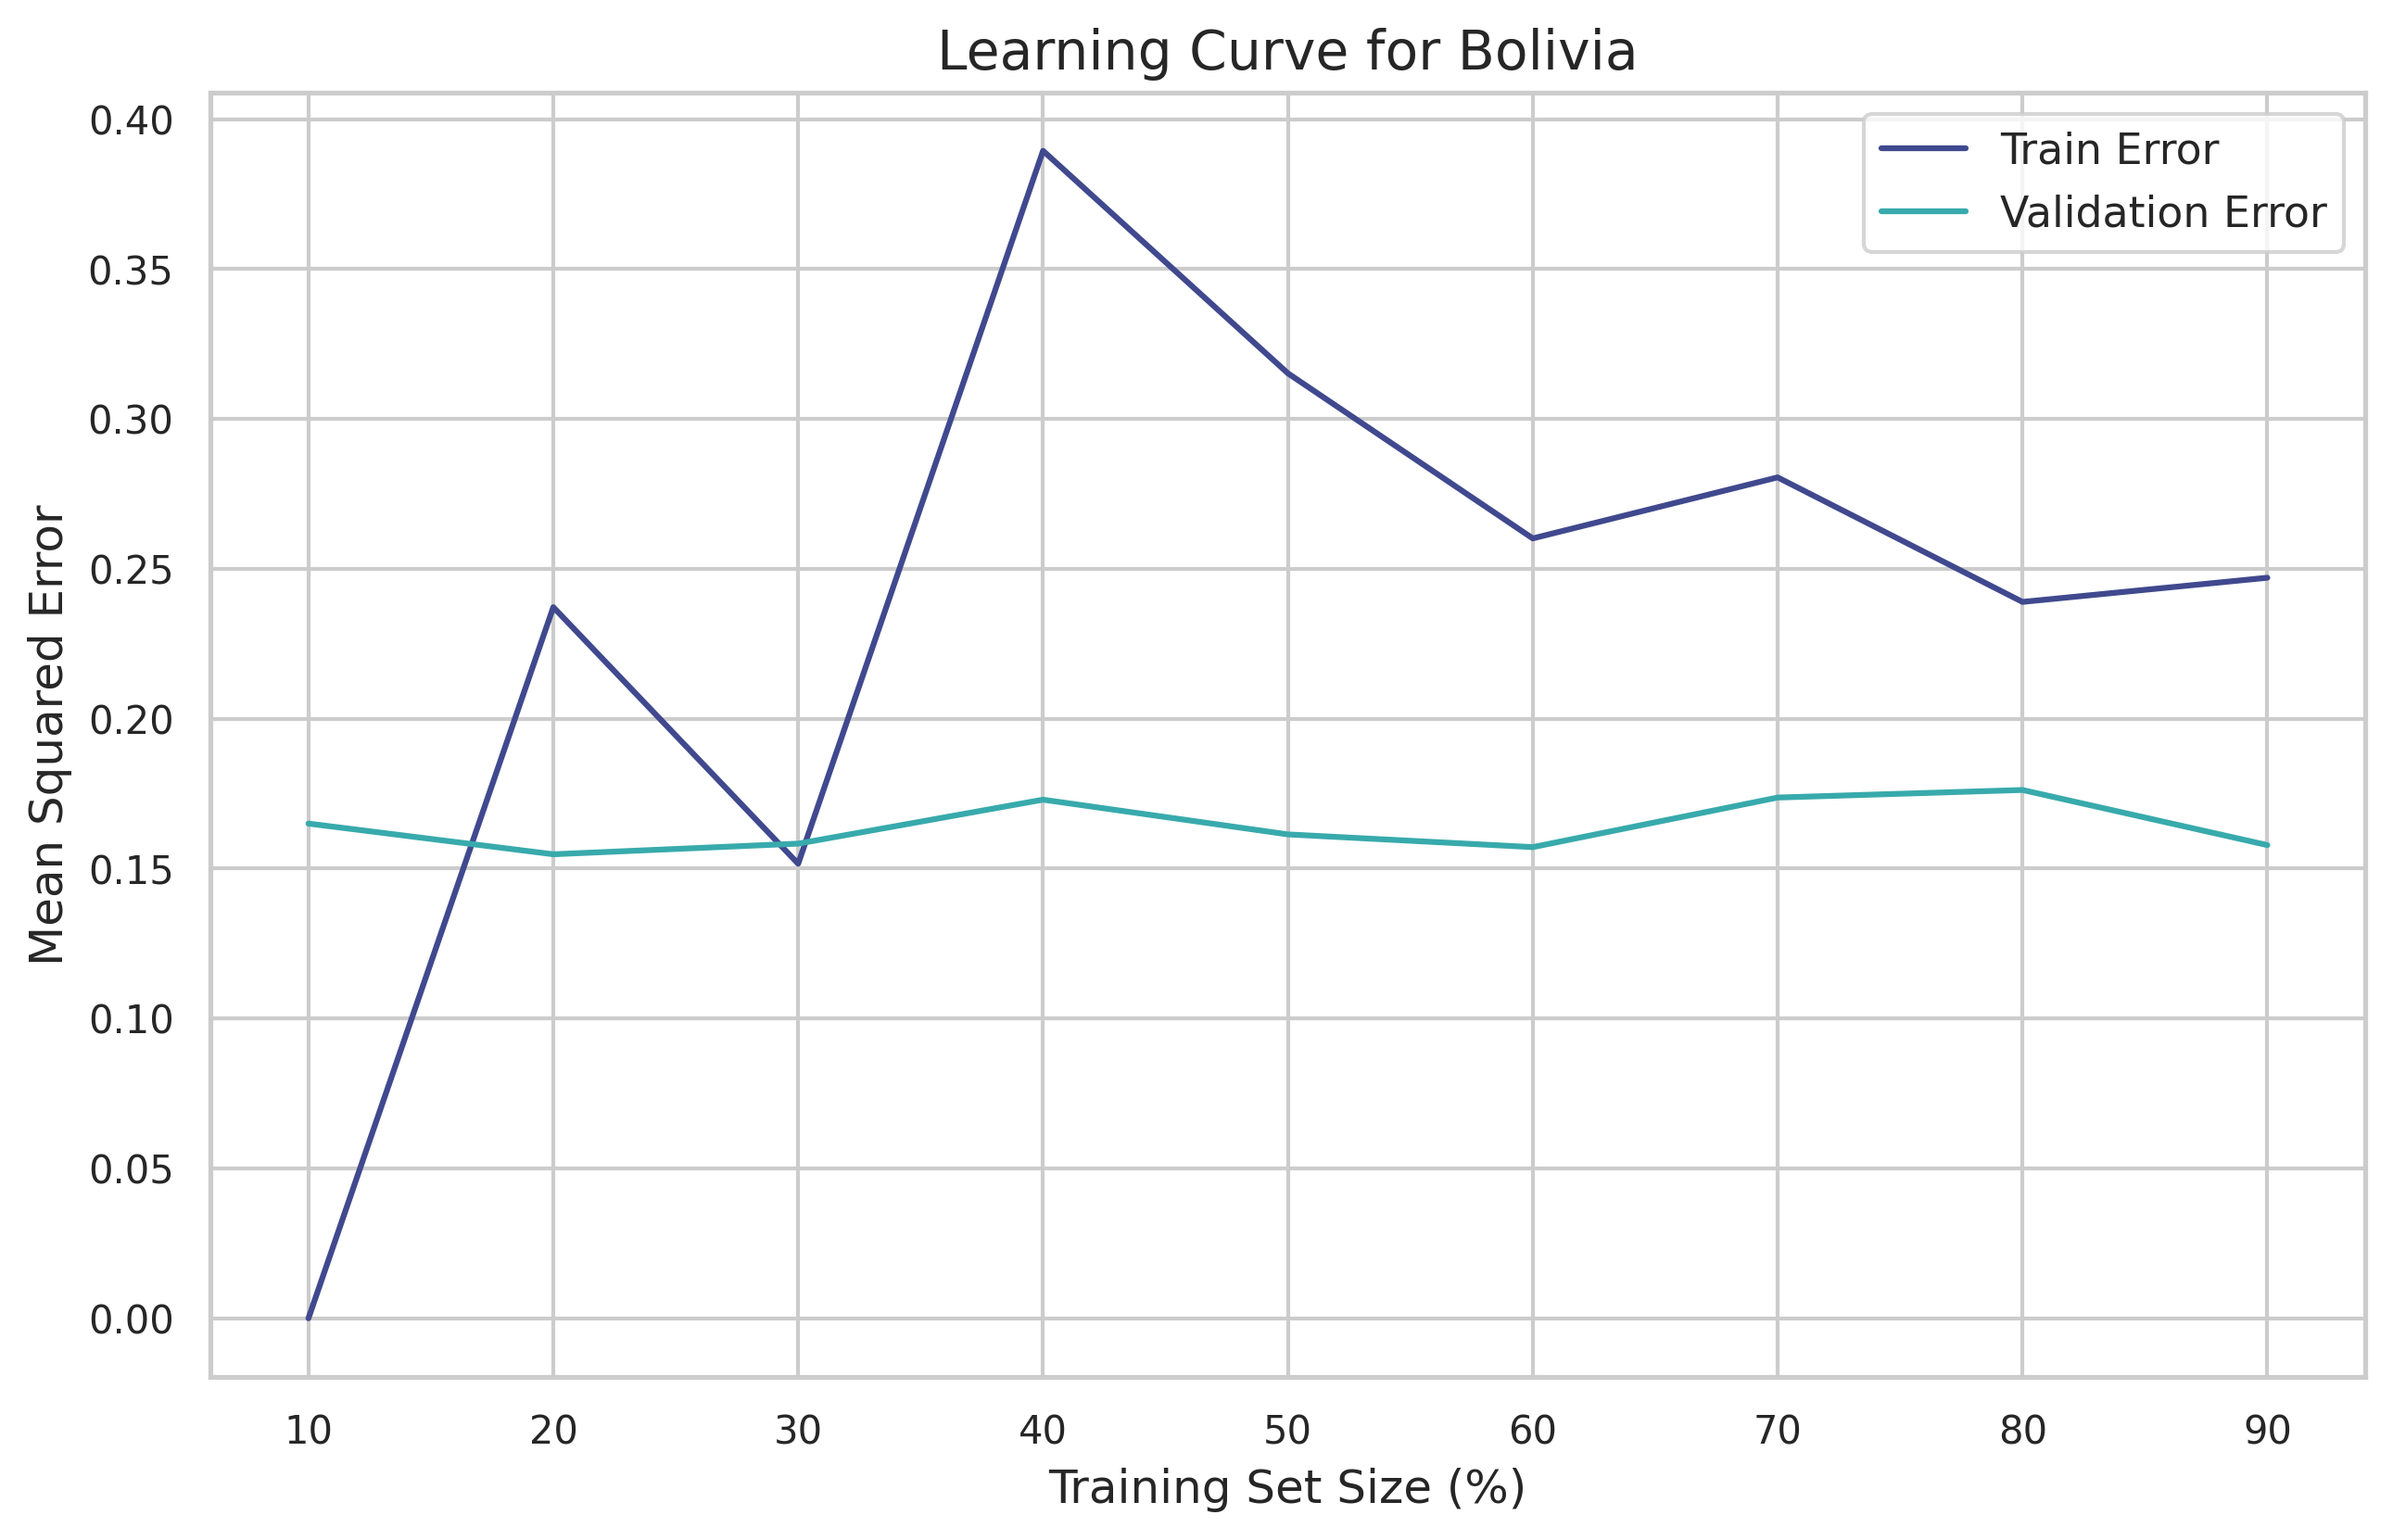
\includegraphics[width=0.8\textwidth]{/Users/sarabcidf/Desktop/ASDS/Dissertation/FinalScripts/CallanByCountry/Bolivia_learning_curve.png}
	\end{figure}
	
	\newpage
	
	\subsection{Chile}
	\begin{figure}[H]
		\centering
		\caption{Feature Importance for Chile Model}
		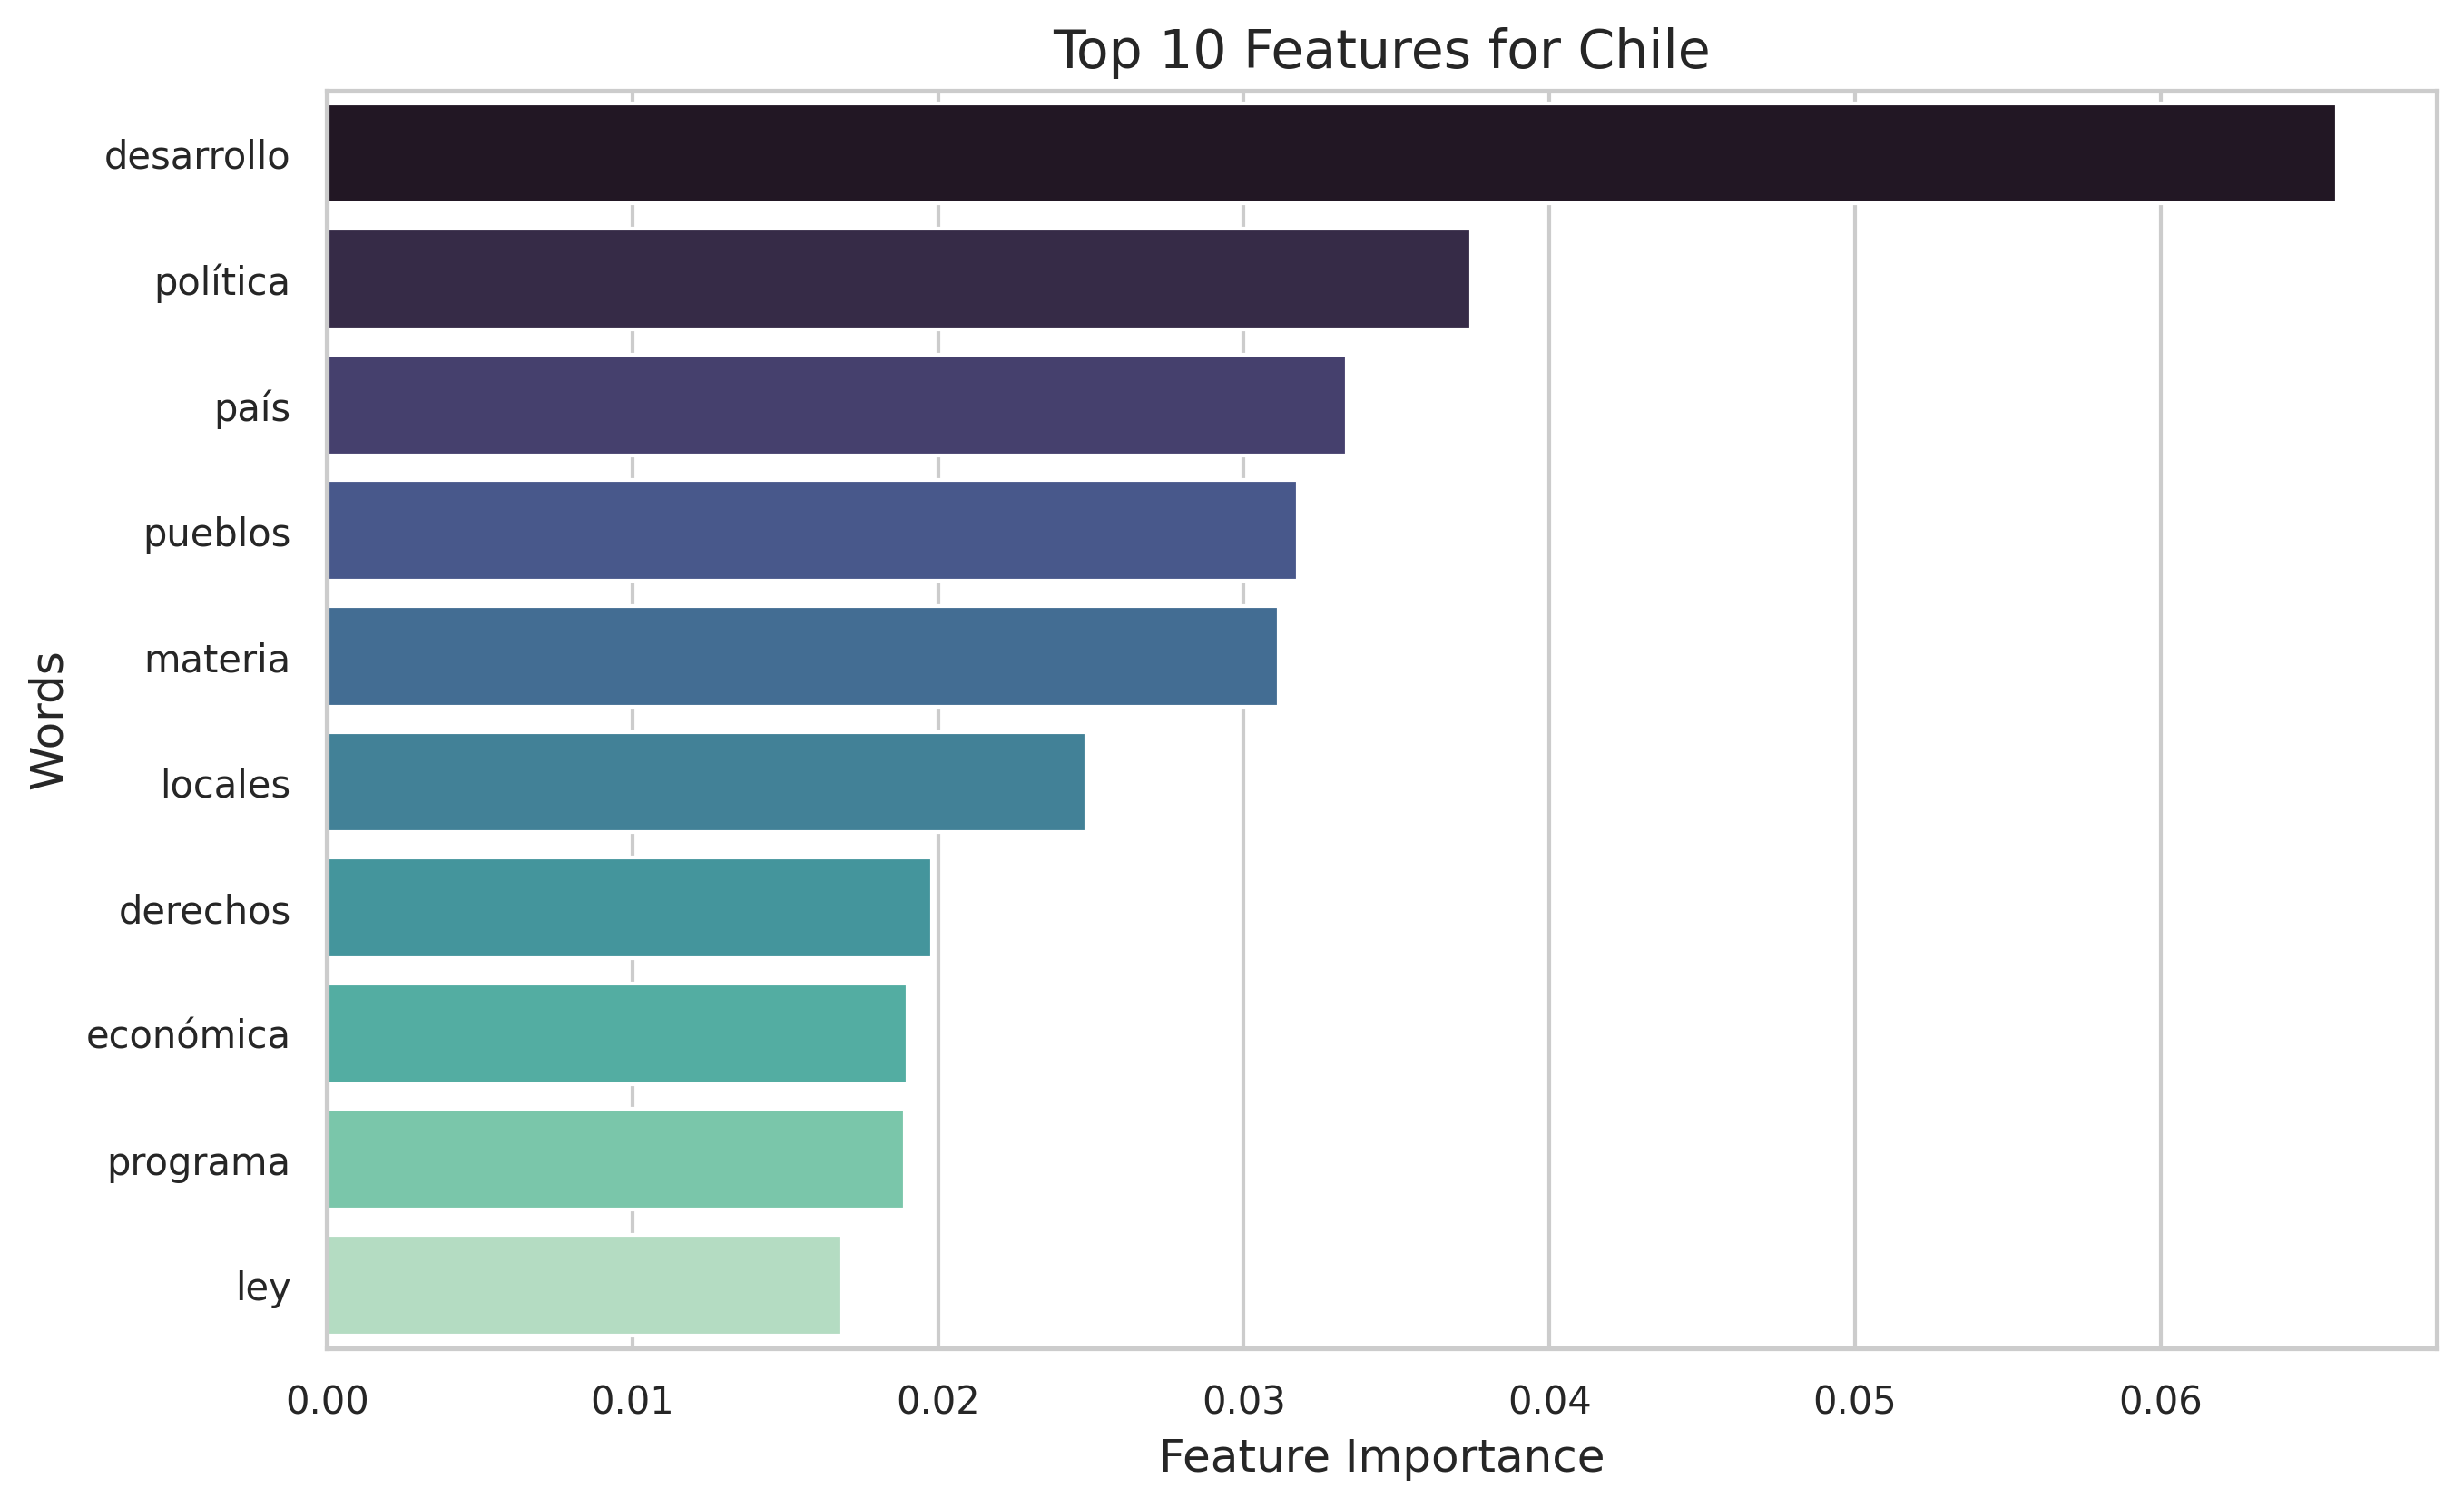
\includegraphics[width=0.8\textwidth]{/Users/sarabcidf/Desktop/ASDS/Dissertation/FinalScripts/CallanByCountry/Chile_feature_importance.png}
	\end{figure}
	\begin{figure}[H]
		\centering
		\caption{Error Rate for Chile Model}
		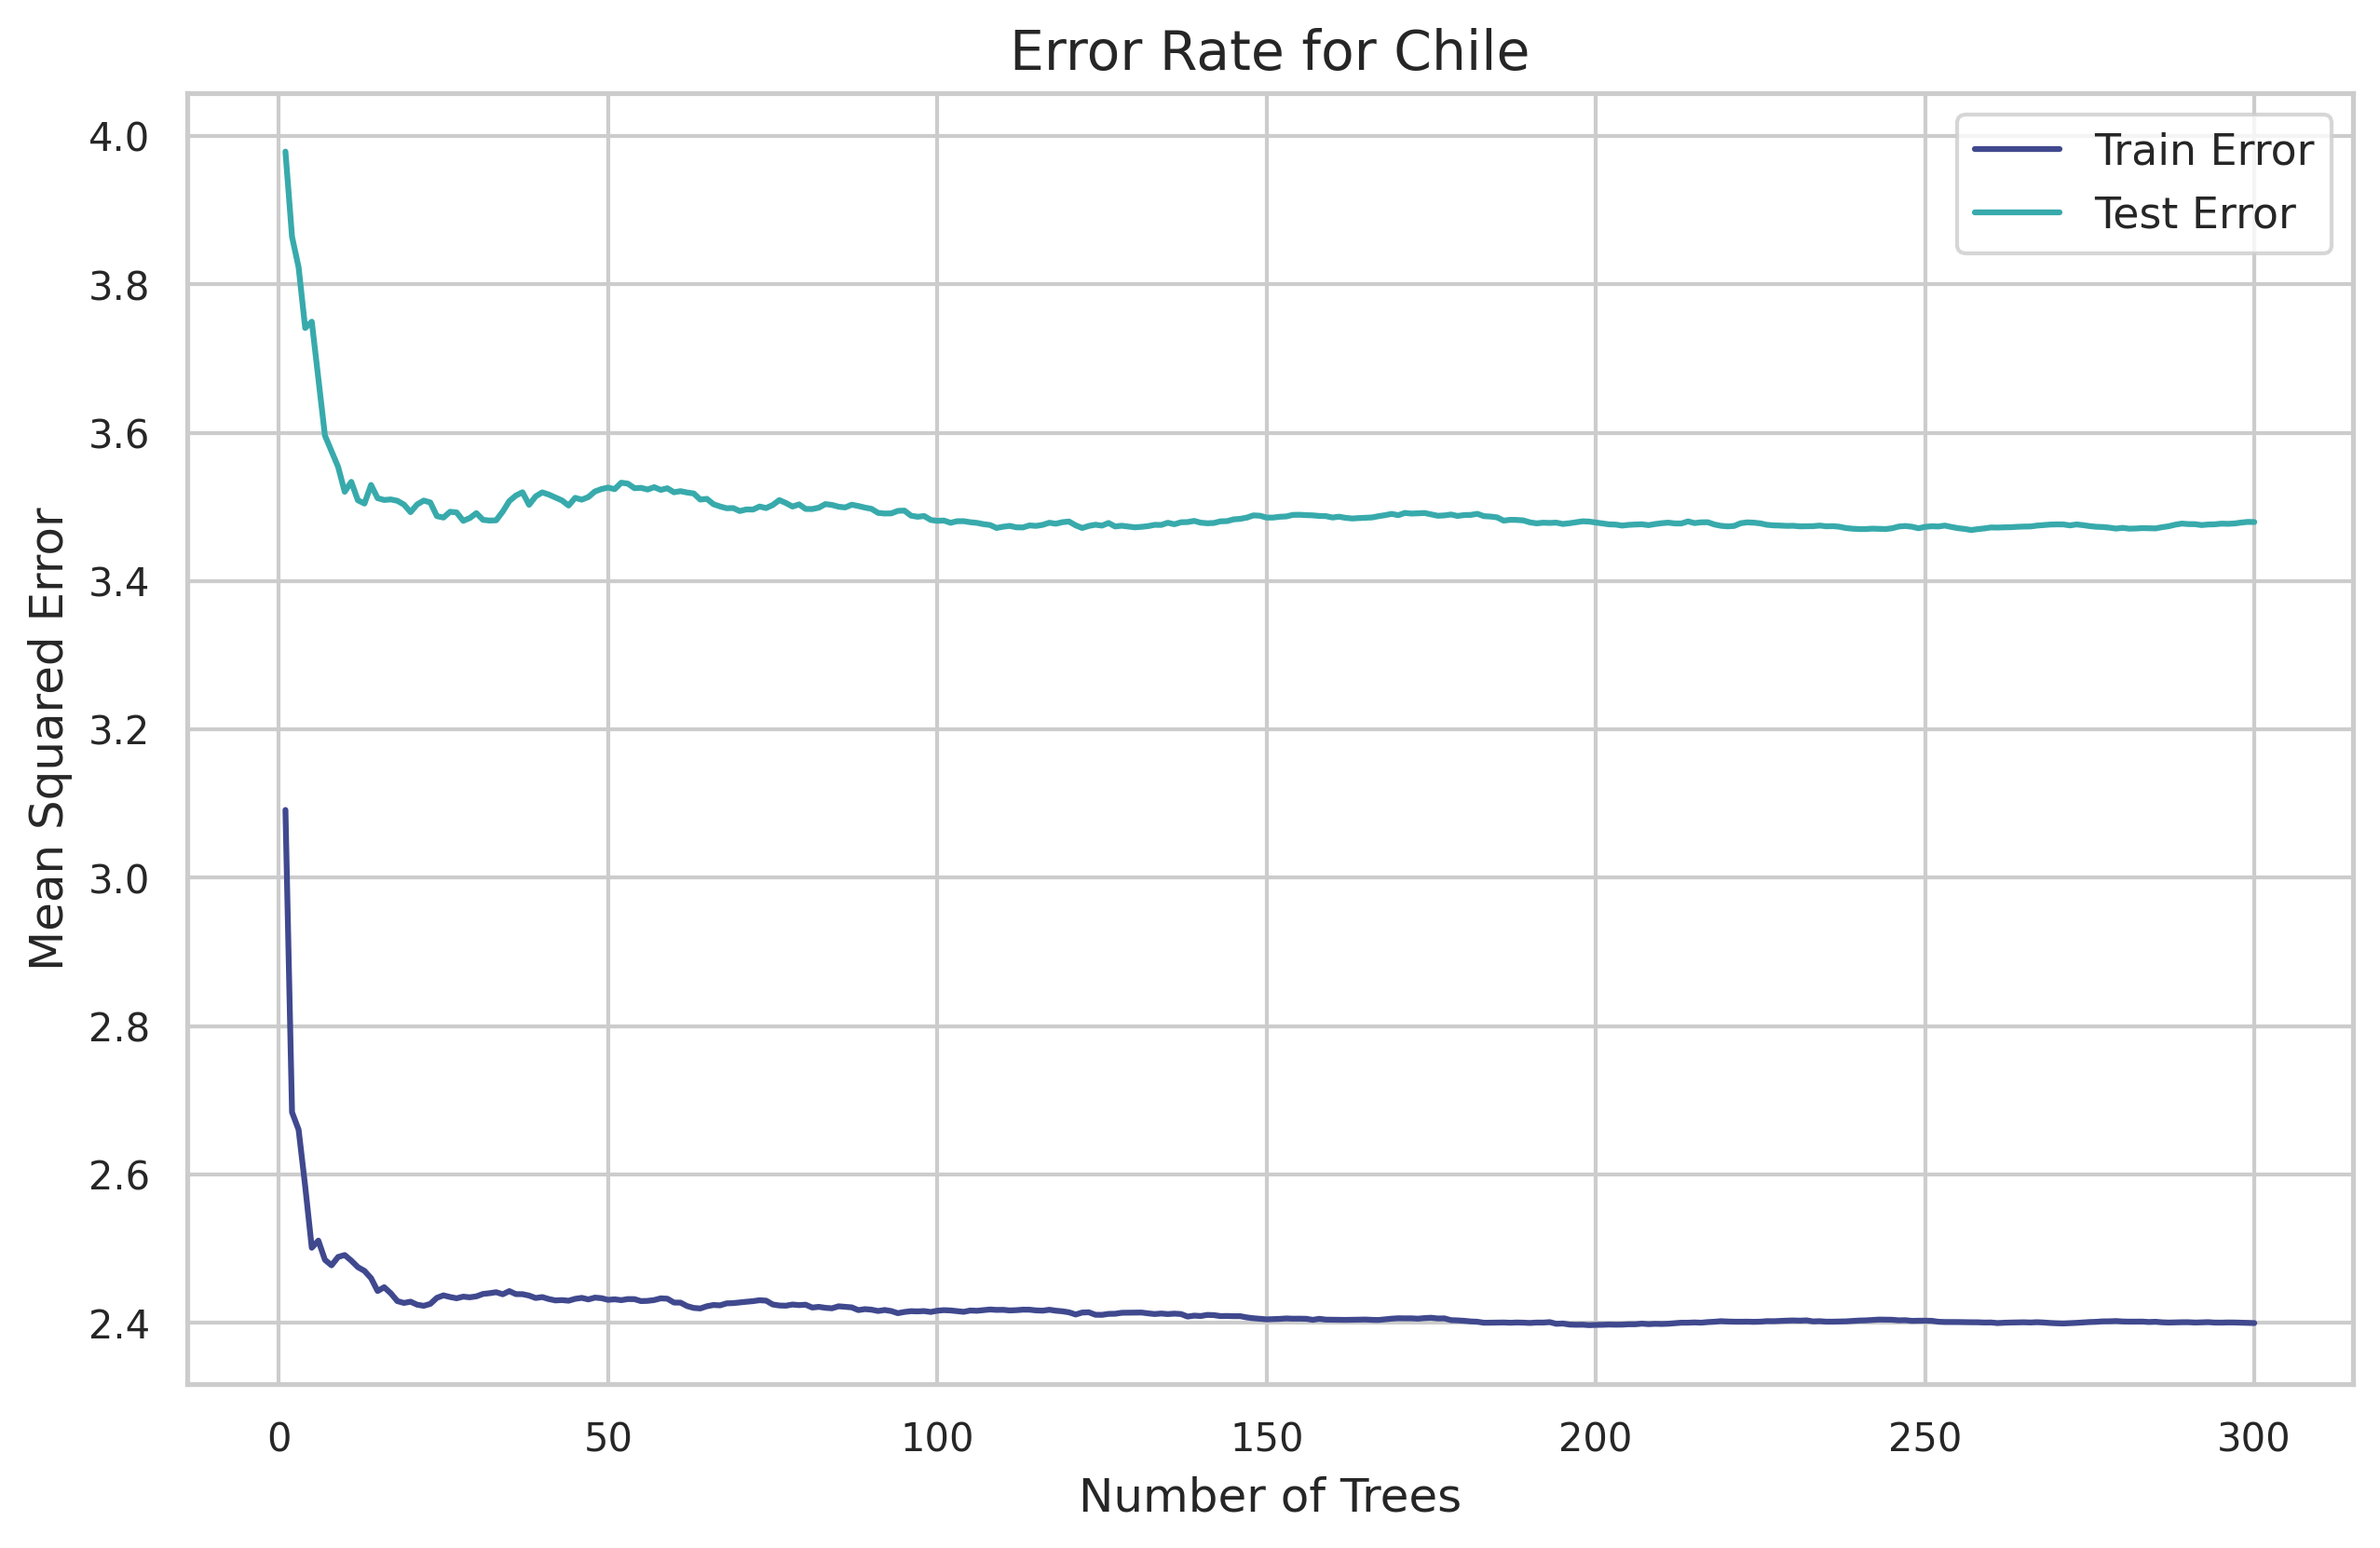
\includegraphics[width=0.8\textwidth]{/Users/sarabcidf/Desktop/ASDS/Dissertation/FinalScripts/CallanByCountry/Chile_error_rate.png}
	\end{figure}
	\begin{figure}[H]
		\centering
		\caption{Learning Curve for Chile Model}
		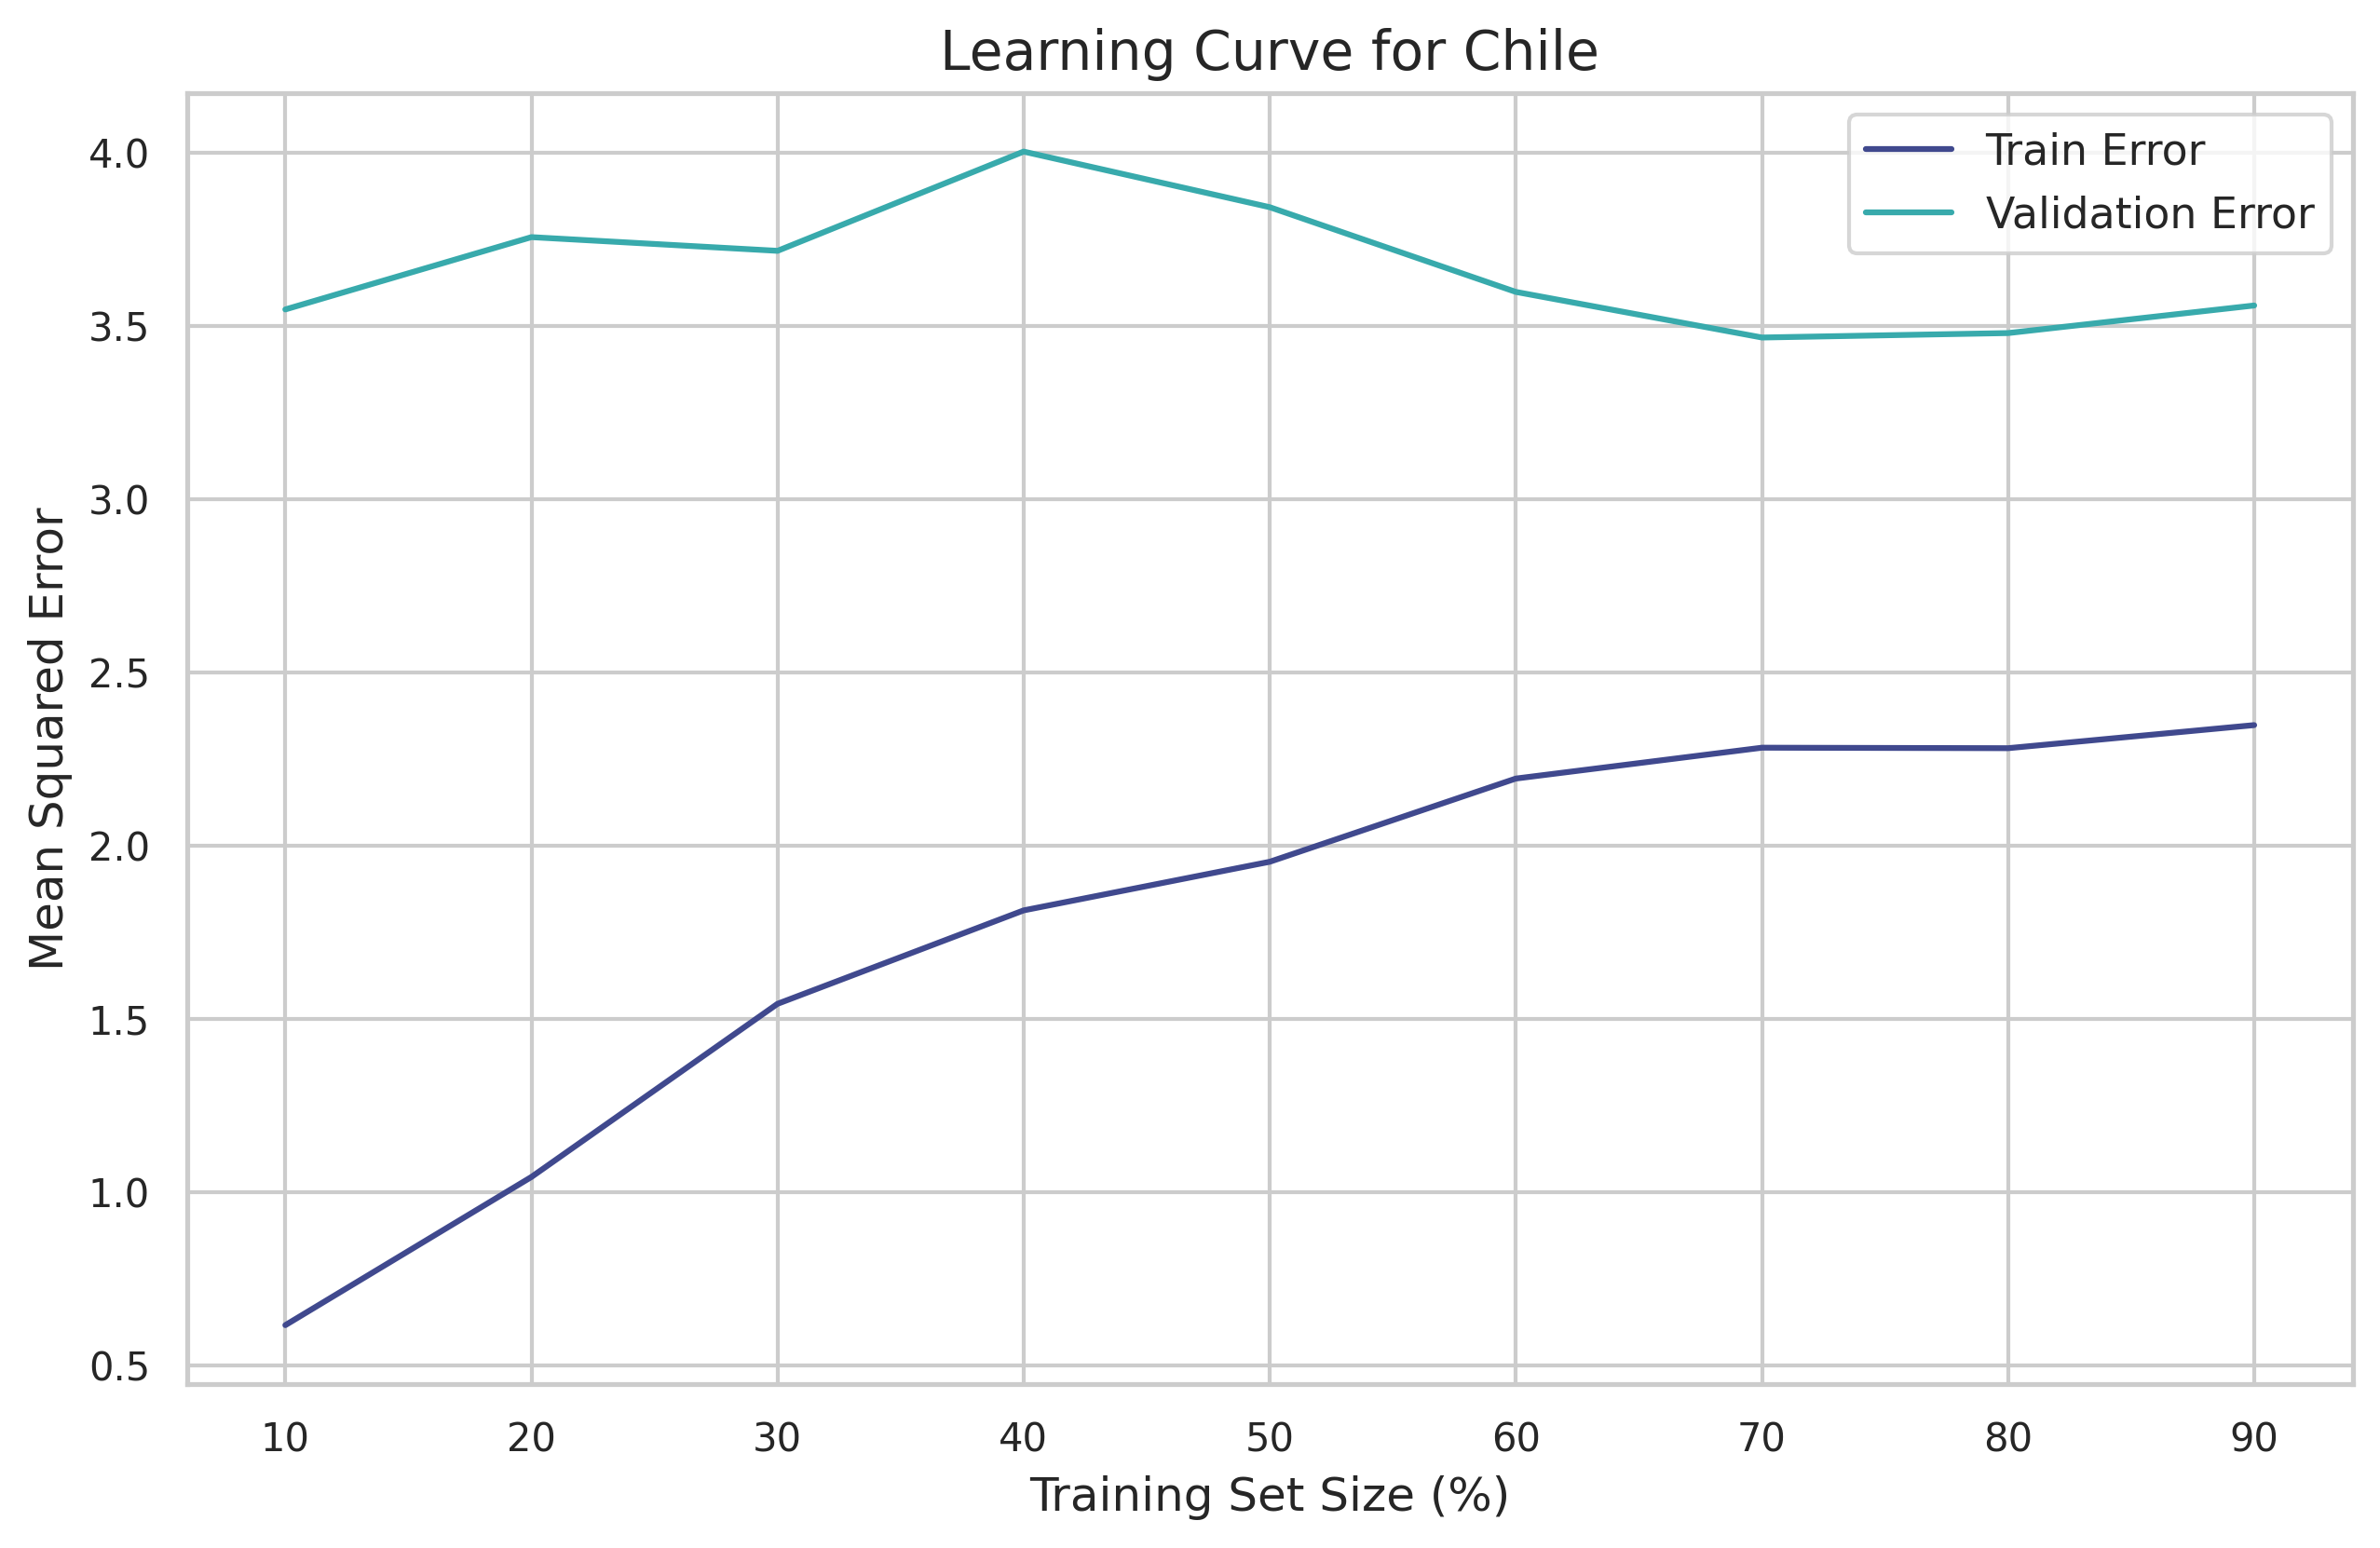
\includegraphics[width=0.8\textwidth]{/Users/sarabcidf/Desktop/ASDS/Dissertation/FinalScripts/CallanByCountry/Chile_learning_curve.png}
	\end{figure}
	
	\newpage
	
	\subsection{Colombia}
	\begin{figure}[H]
		\centering
		\caption{Feature Importance for Colombia Model}
		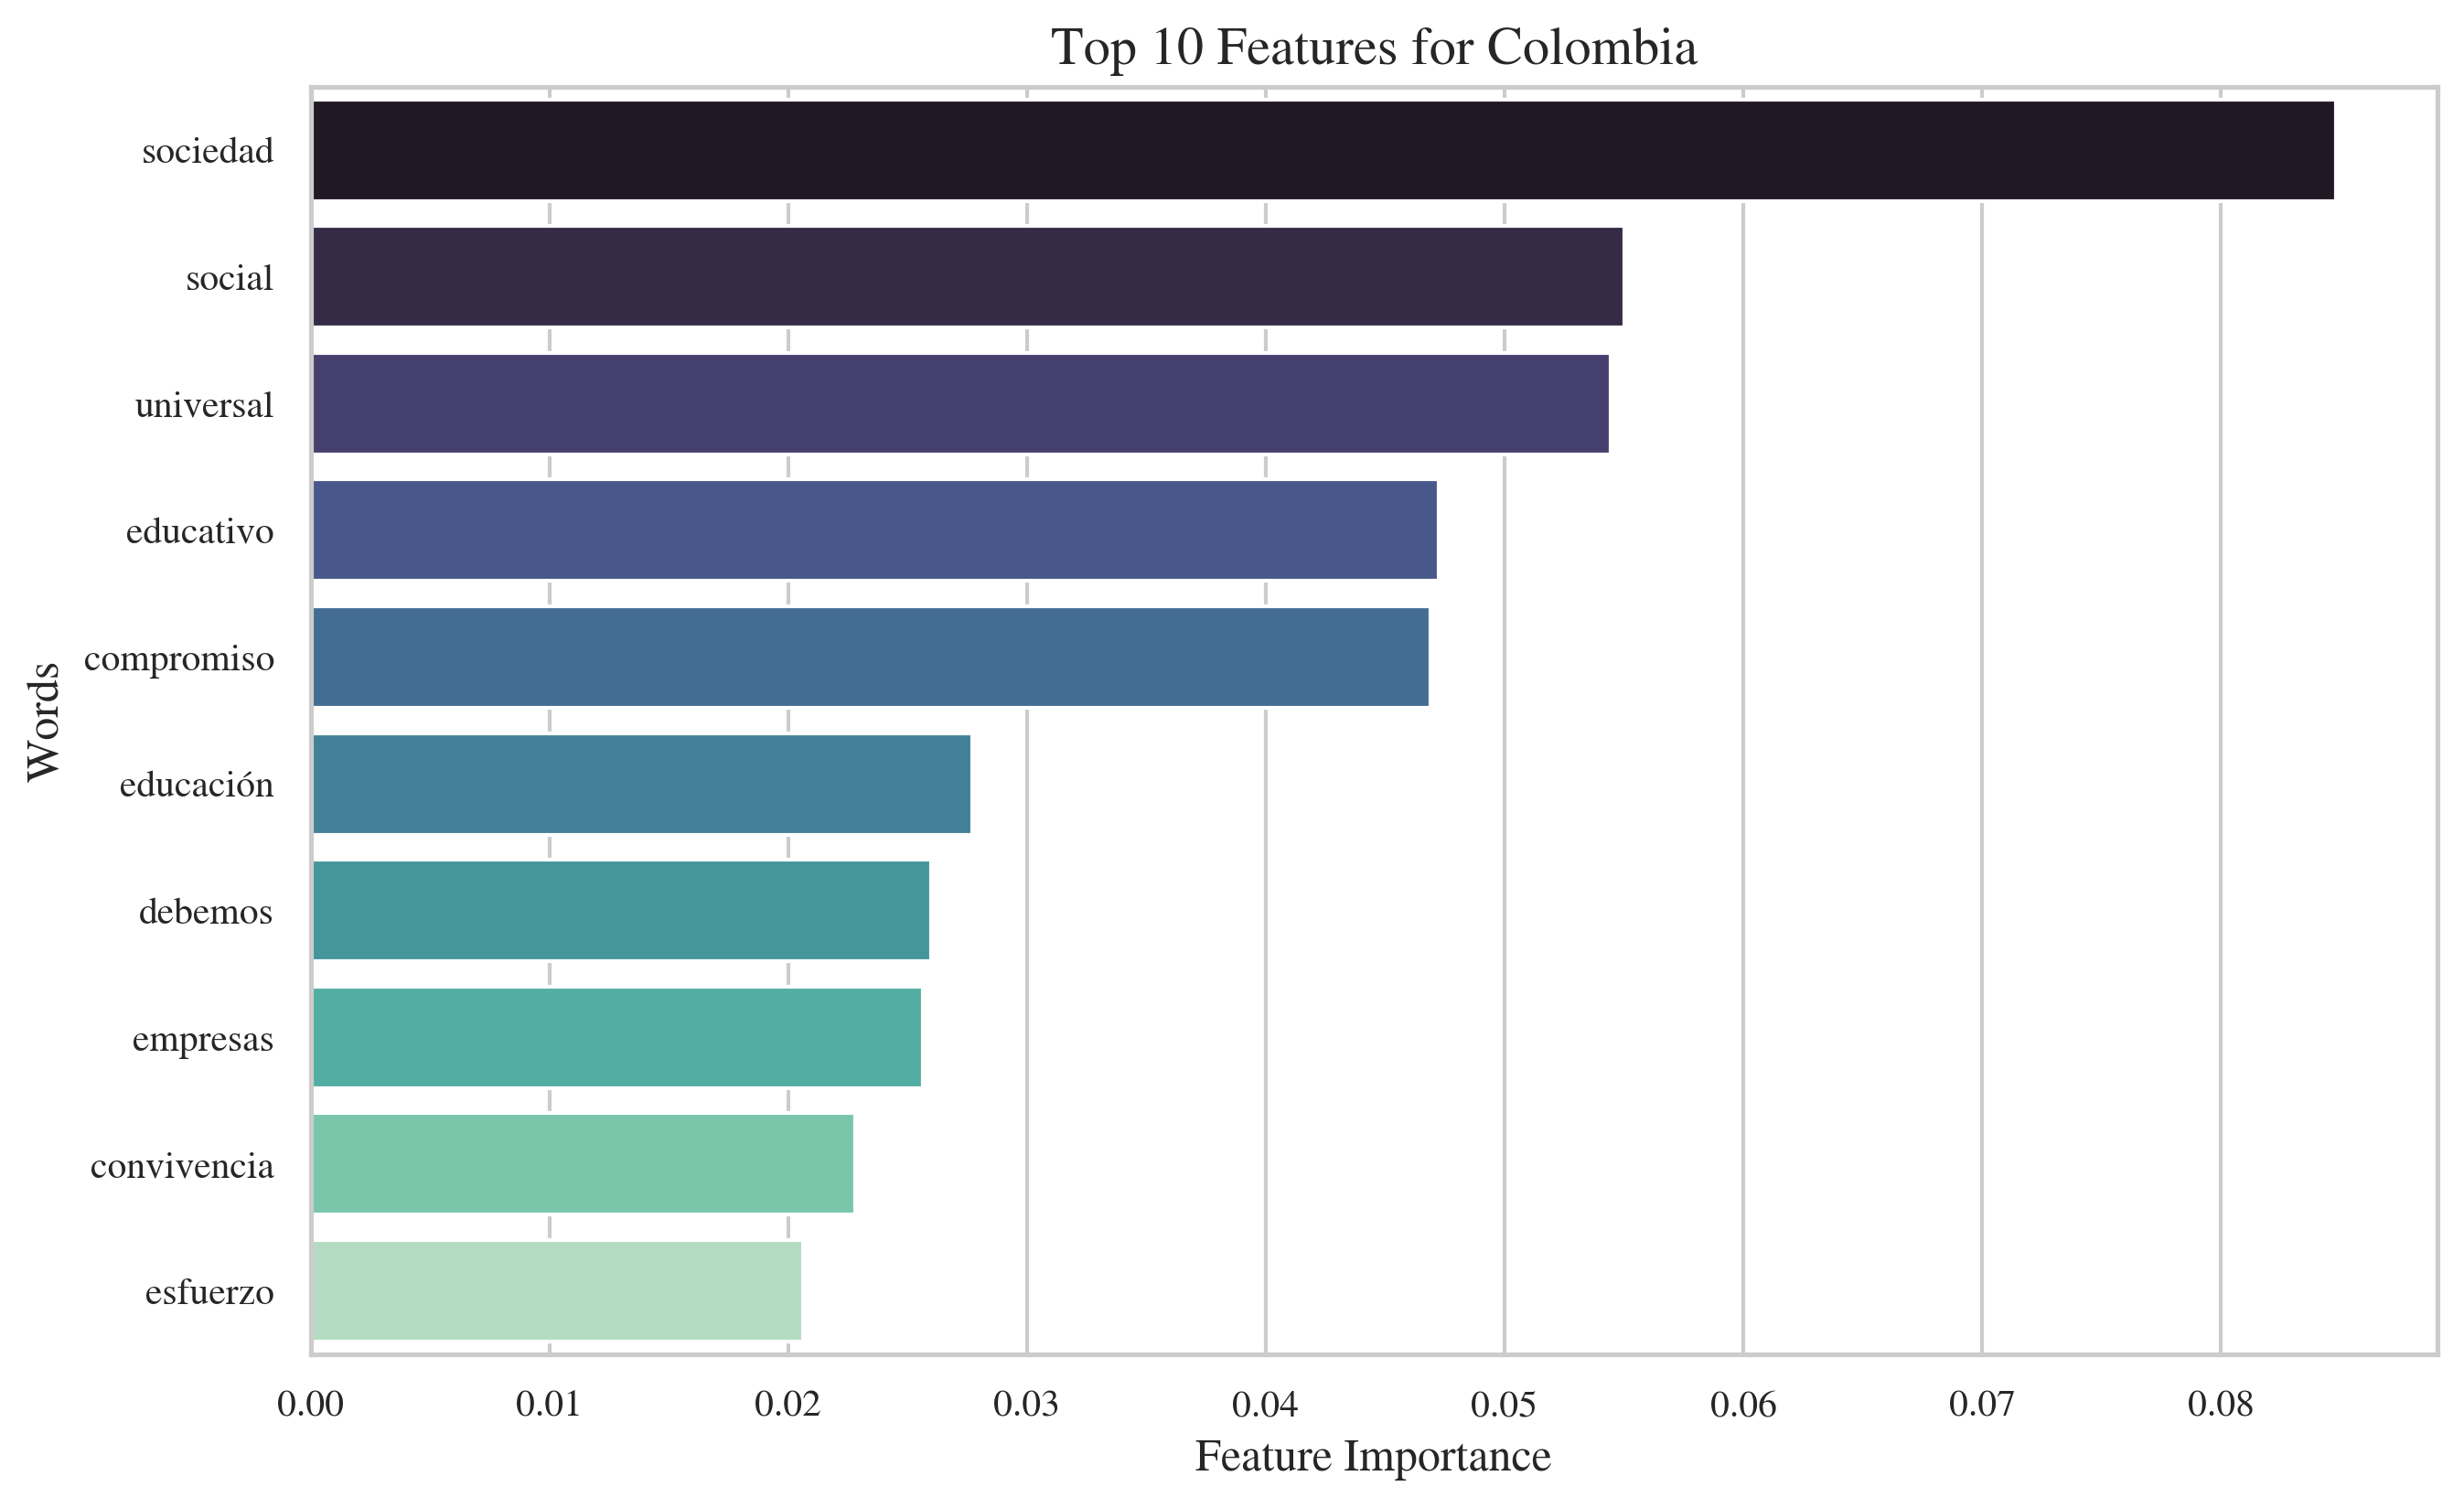
\includegraphics[width=0.8\textwidth]{/Users/sarabcidf/Desktop/ASDS/Dissertation/FinalScripts/CallanByCountry/Colombia_feature_importance.png}
	\end{figure}
	\begin{figure}[H]
		\centering
		\caption{Error Rate for Colombia Model}
		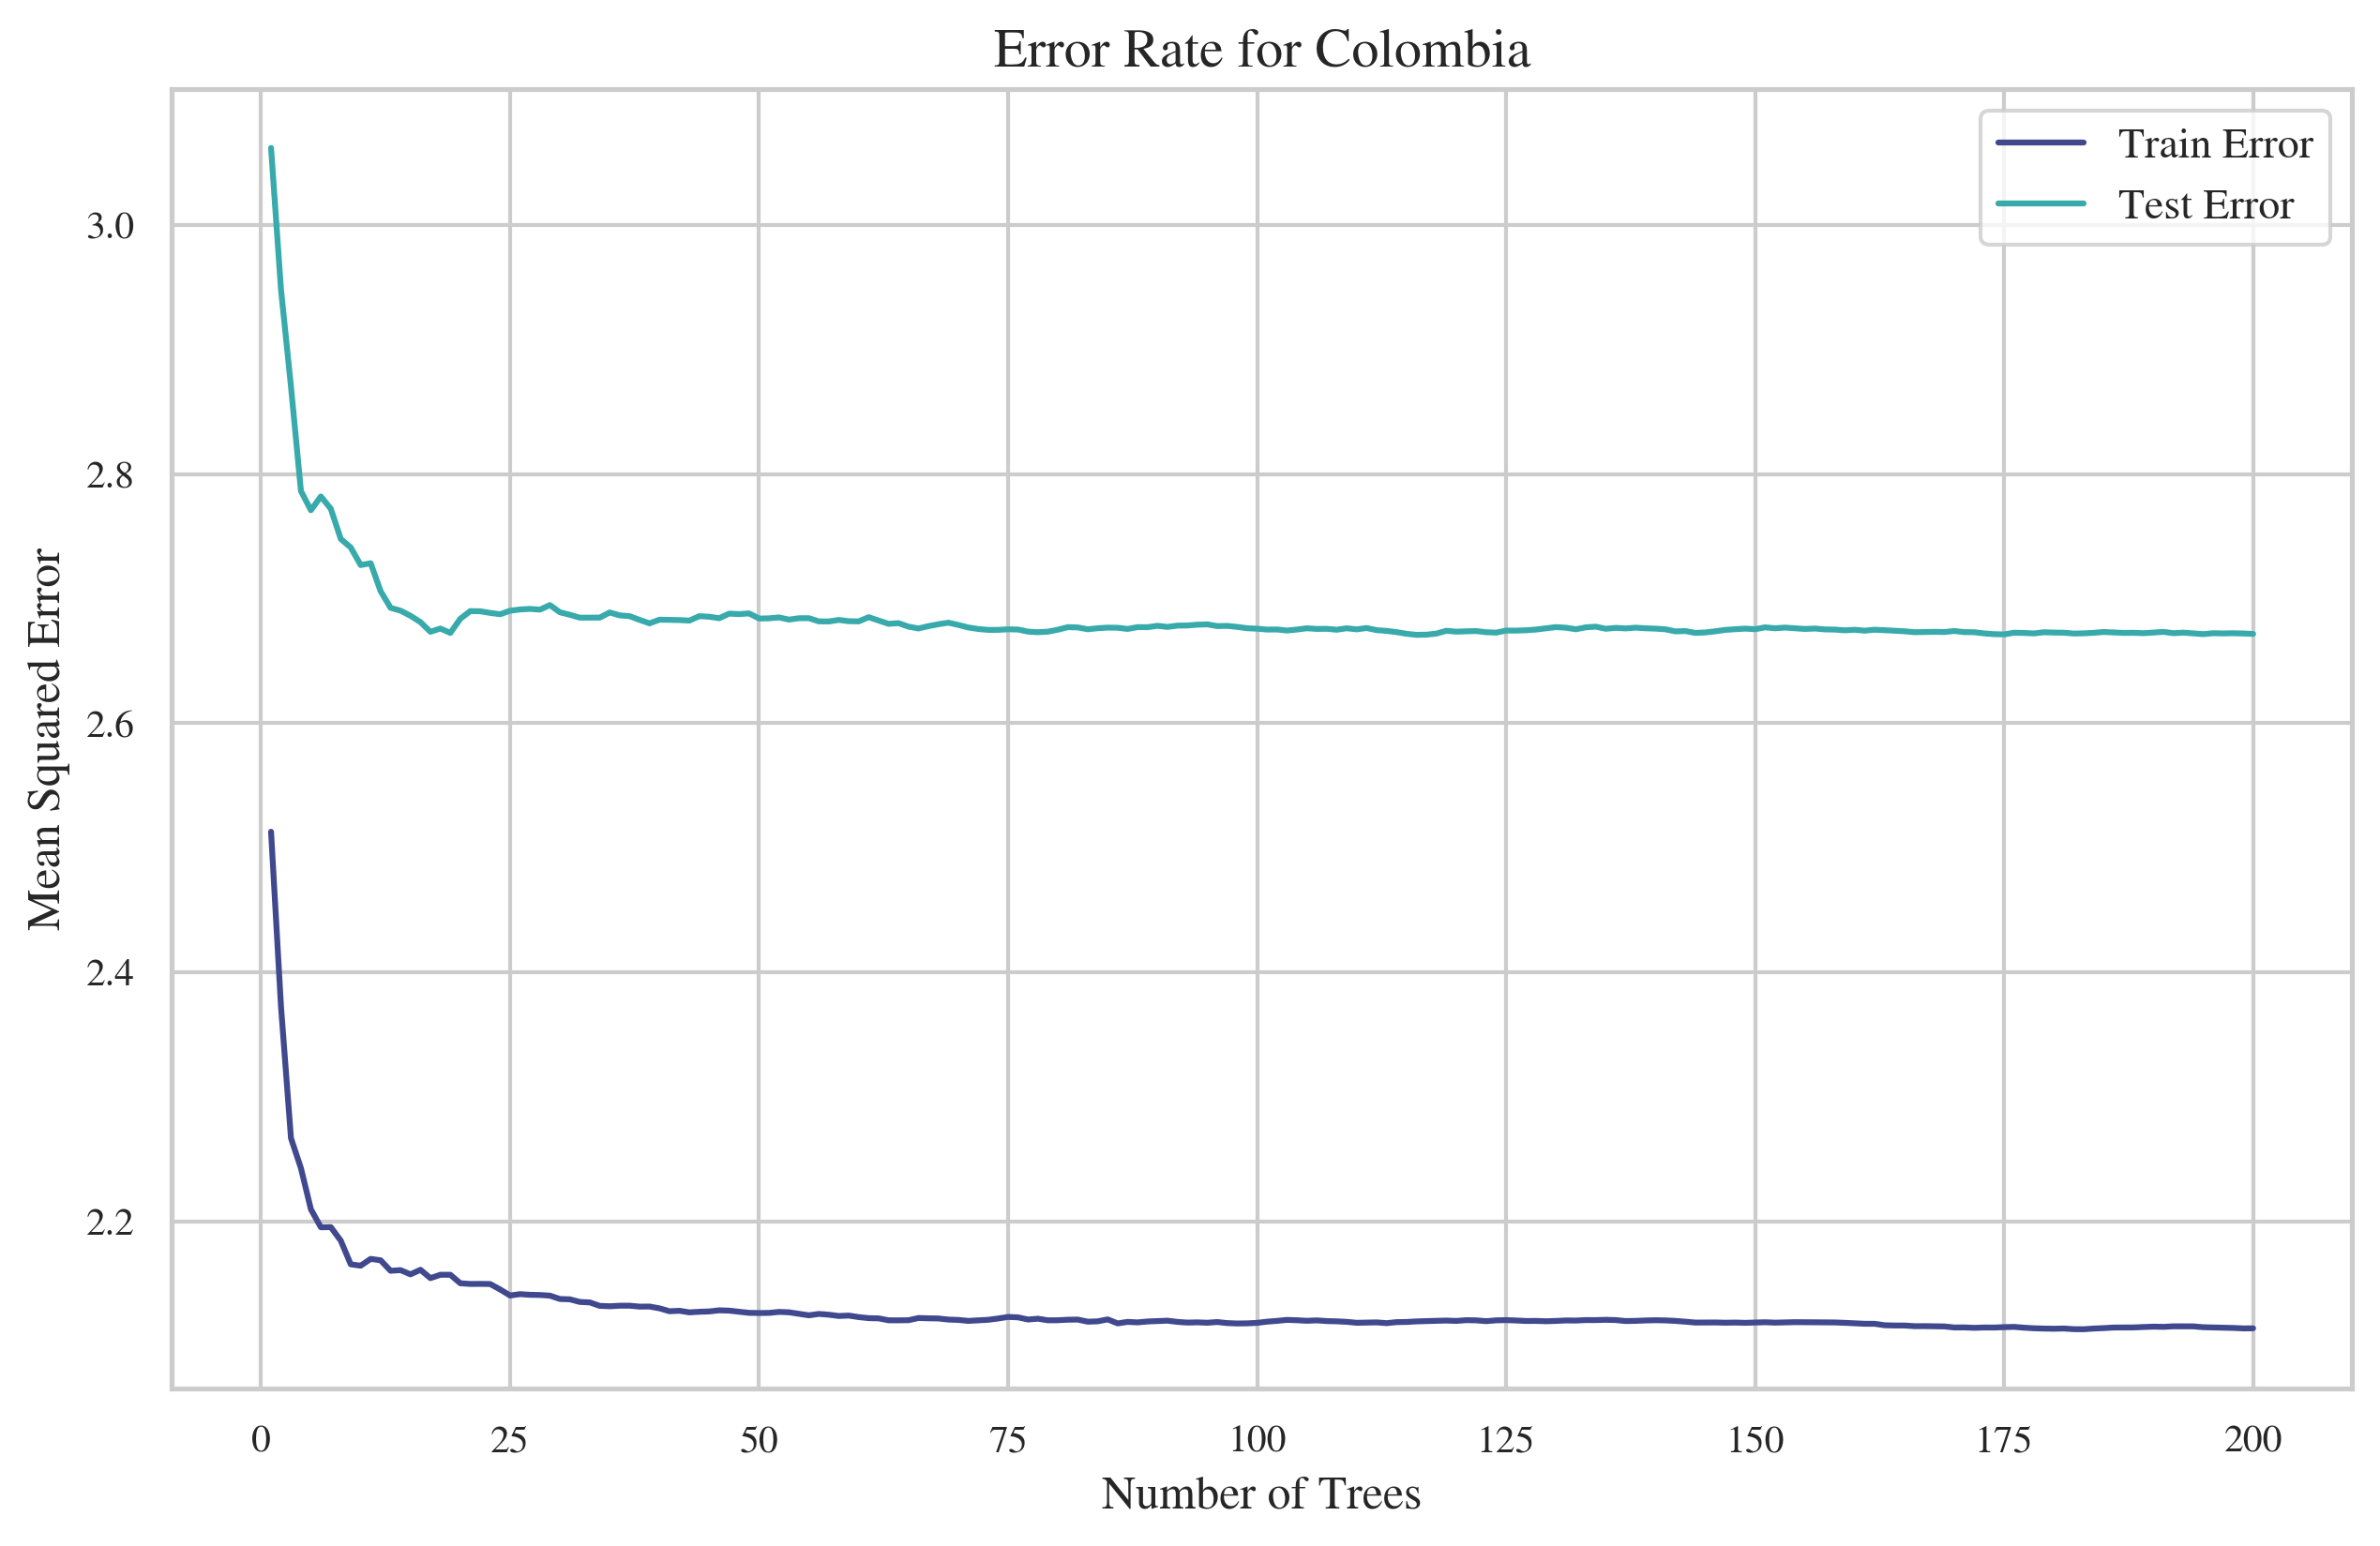
\includegraphics[width=0.8\textwidth]{/Users/sarabcidf/Desktop/ASDS/Dissertation/FinalScripts/CallanByCountry/Colombia_error_rate.png}
	\end{figure}
	\begin{figure}[H]
		\centering
		\caption{Learning Curve for Colombia Model}
		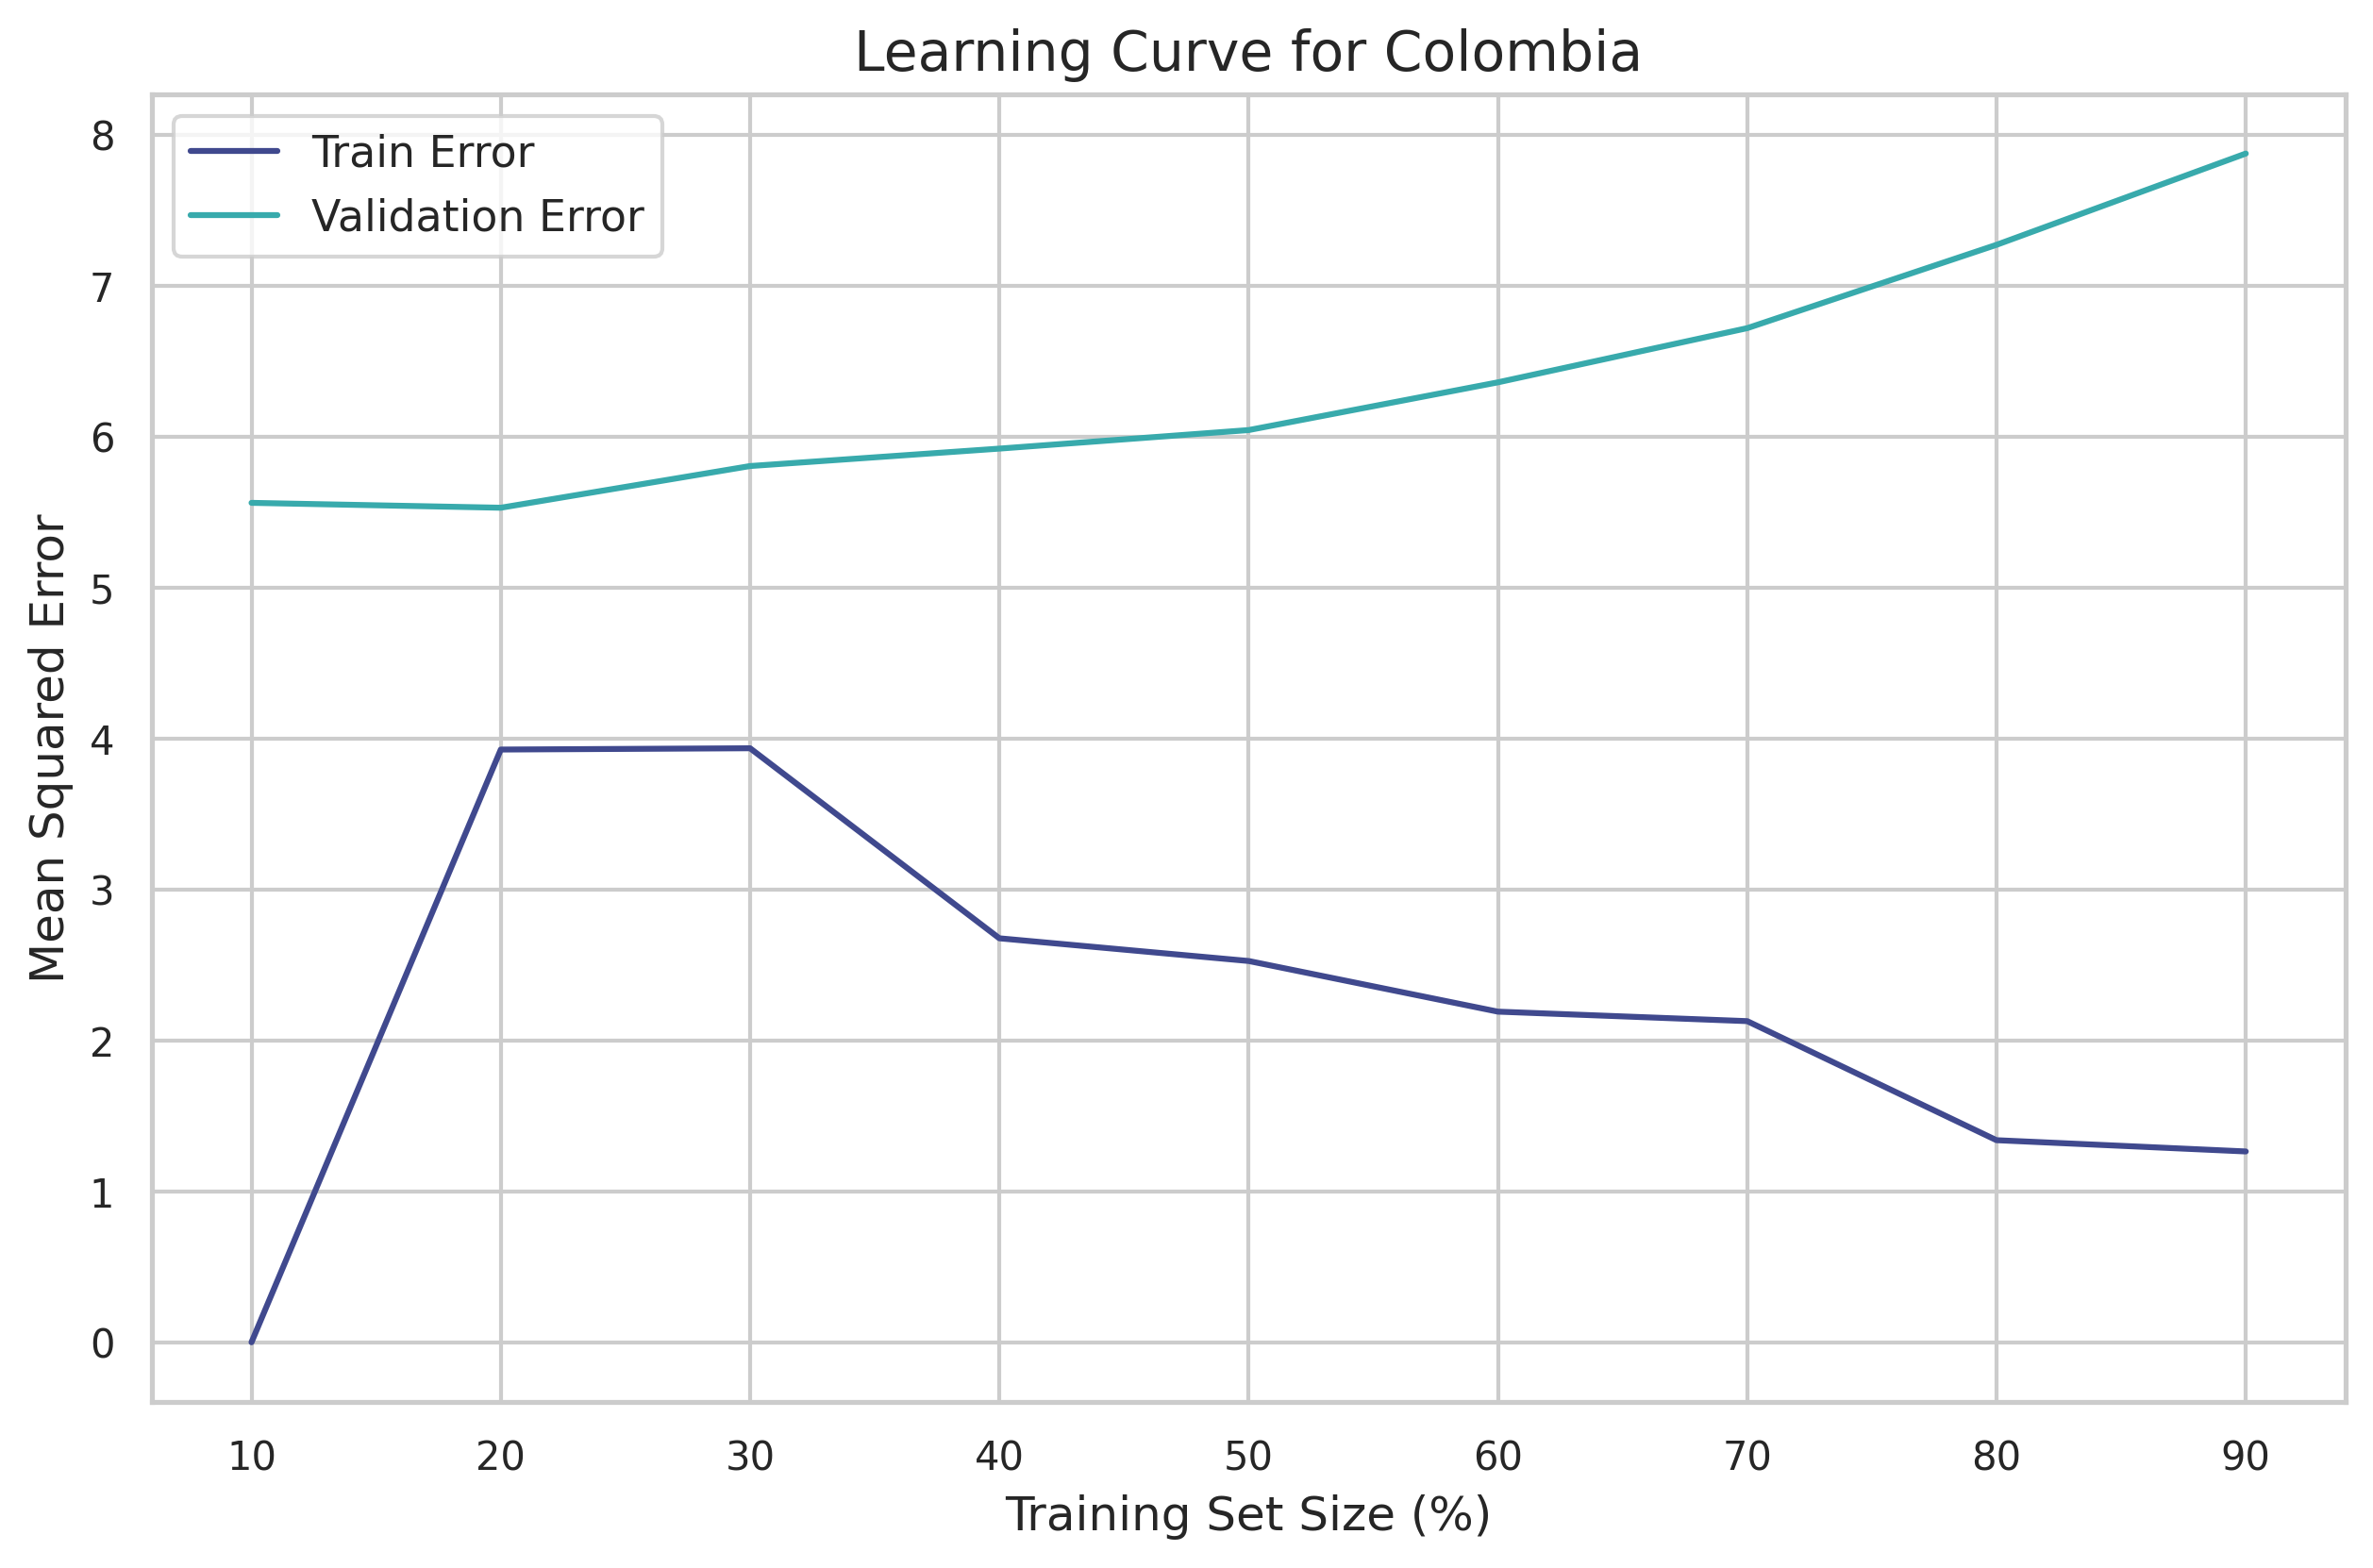
\includegraphics[width=0.8\textwidth]{/Users/sarabcidf/Desktop/ASDS/Dissertation/FinalScripts/CallanByCountry/Colombia_learning_curve.png}
	\end{figure}
	
	\newpage
	
	\subsection{Costa Rica}
	\begin{figure}[H]
		\centering
		\caption{Feature Importance for Costa Rica Model}
		\includegraphics[width=0.8\textwidth]{/Users/sarabcidf/Desktop/ASDS/Dissertation/FinalScripts/CallanByCountry/Costa  Rica_feature_importance.png}
	\end{figure}
	\begin{figure}[H]
		\centering
		\caption{Error Rate for Costa Rica Model}
		\includegraphics[width=0.8\textwidth]{/Users/sarabcidf/Desktop/ASDS/Dissertation/FinalScripts/CallanByCountry/Costa  Rica_error_rate.png}
	\end{figure}
	\begin{figure}[H]
		\centering
		\caption{Learning Curve for Costa Rica Model}
		\includegraphics[width=0.8\textwidth]{/Users/sarabcidf/Desktop/ASDS/Dissertation/FinalScripts/CallanByCountry/Costa  Rica_learning_curve.png}
	\end{figure}
	
	\newpage
	
	\subsection{D. Republic}
	\begin{figure}[H]
		\centering
		\caption{Feature Importance for D. Republic Model}
		\includegraphics[width=0.8\textwidth]{/Users/sarabcidf/Desktop/ASDS/Dissertation/FinalScripts/CallanByCountry/D.  Republic_feature_importance.png}
	\end{figure}
	\begin{figure}[H]
		\centering
		\caption{Error Rate for D. Republic Model}
		\includegraphics[width=0.8\textwidth]{/Users/sarabcidf/Desktop/ASDS/Dissertation/FinalScripts/CallanByCountry/D.  Republic_error_rate.png}
	\end{figure}
	\begin{figure}[H]
		\centering
		\caption{Learning Curve for D. Republic Model}
		\includegraphics[width=0.8\textwidth]{/Users/sarabcidf/Desktop/ASDS/Dissertation/FinalScripts/CallanByCountry/D.  Republic_learning_curve.png}
	\end{figure}
	
	\newpage
	
	\subsection{Ecuador}
	\begin{figure}[H]
		\centering
		\caption{Feature Importance for Ecuador Model}
		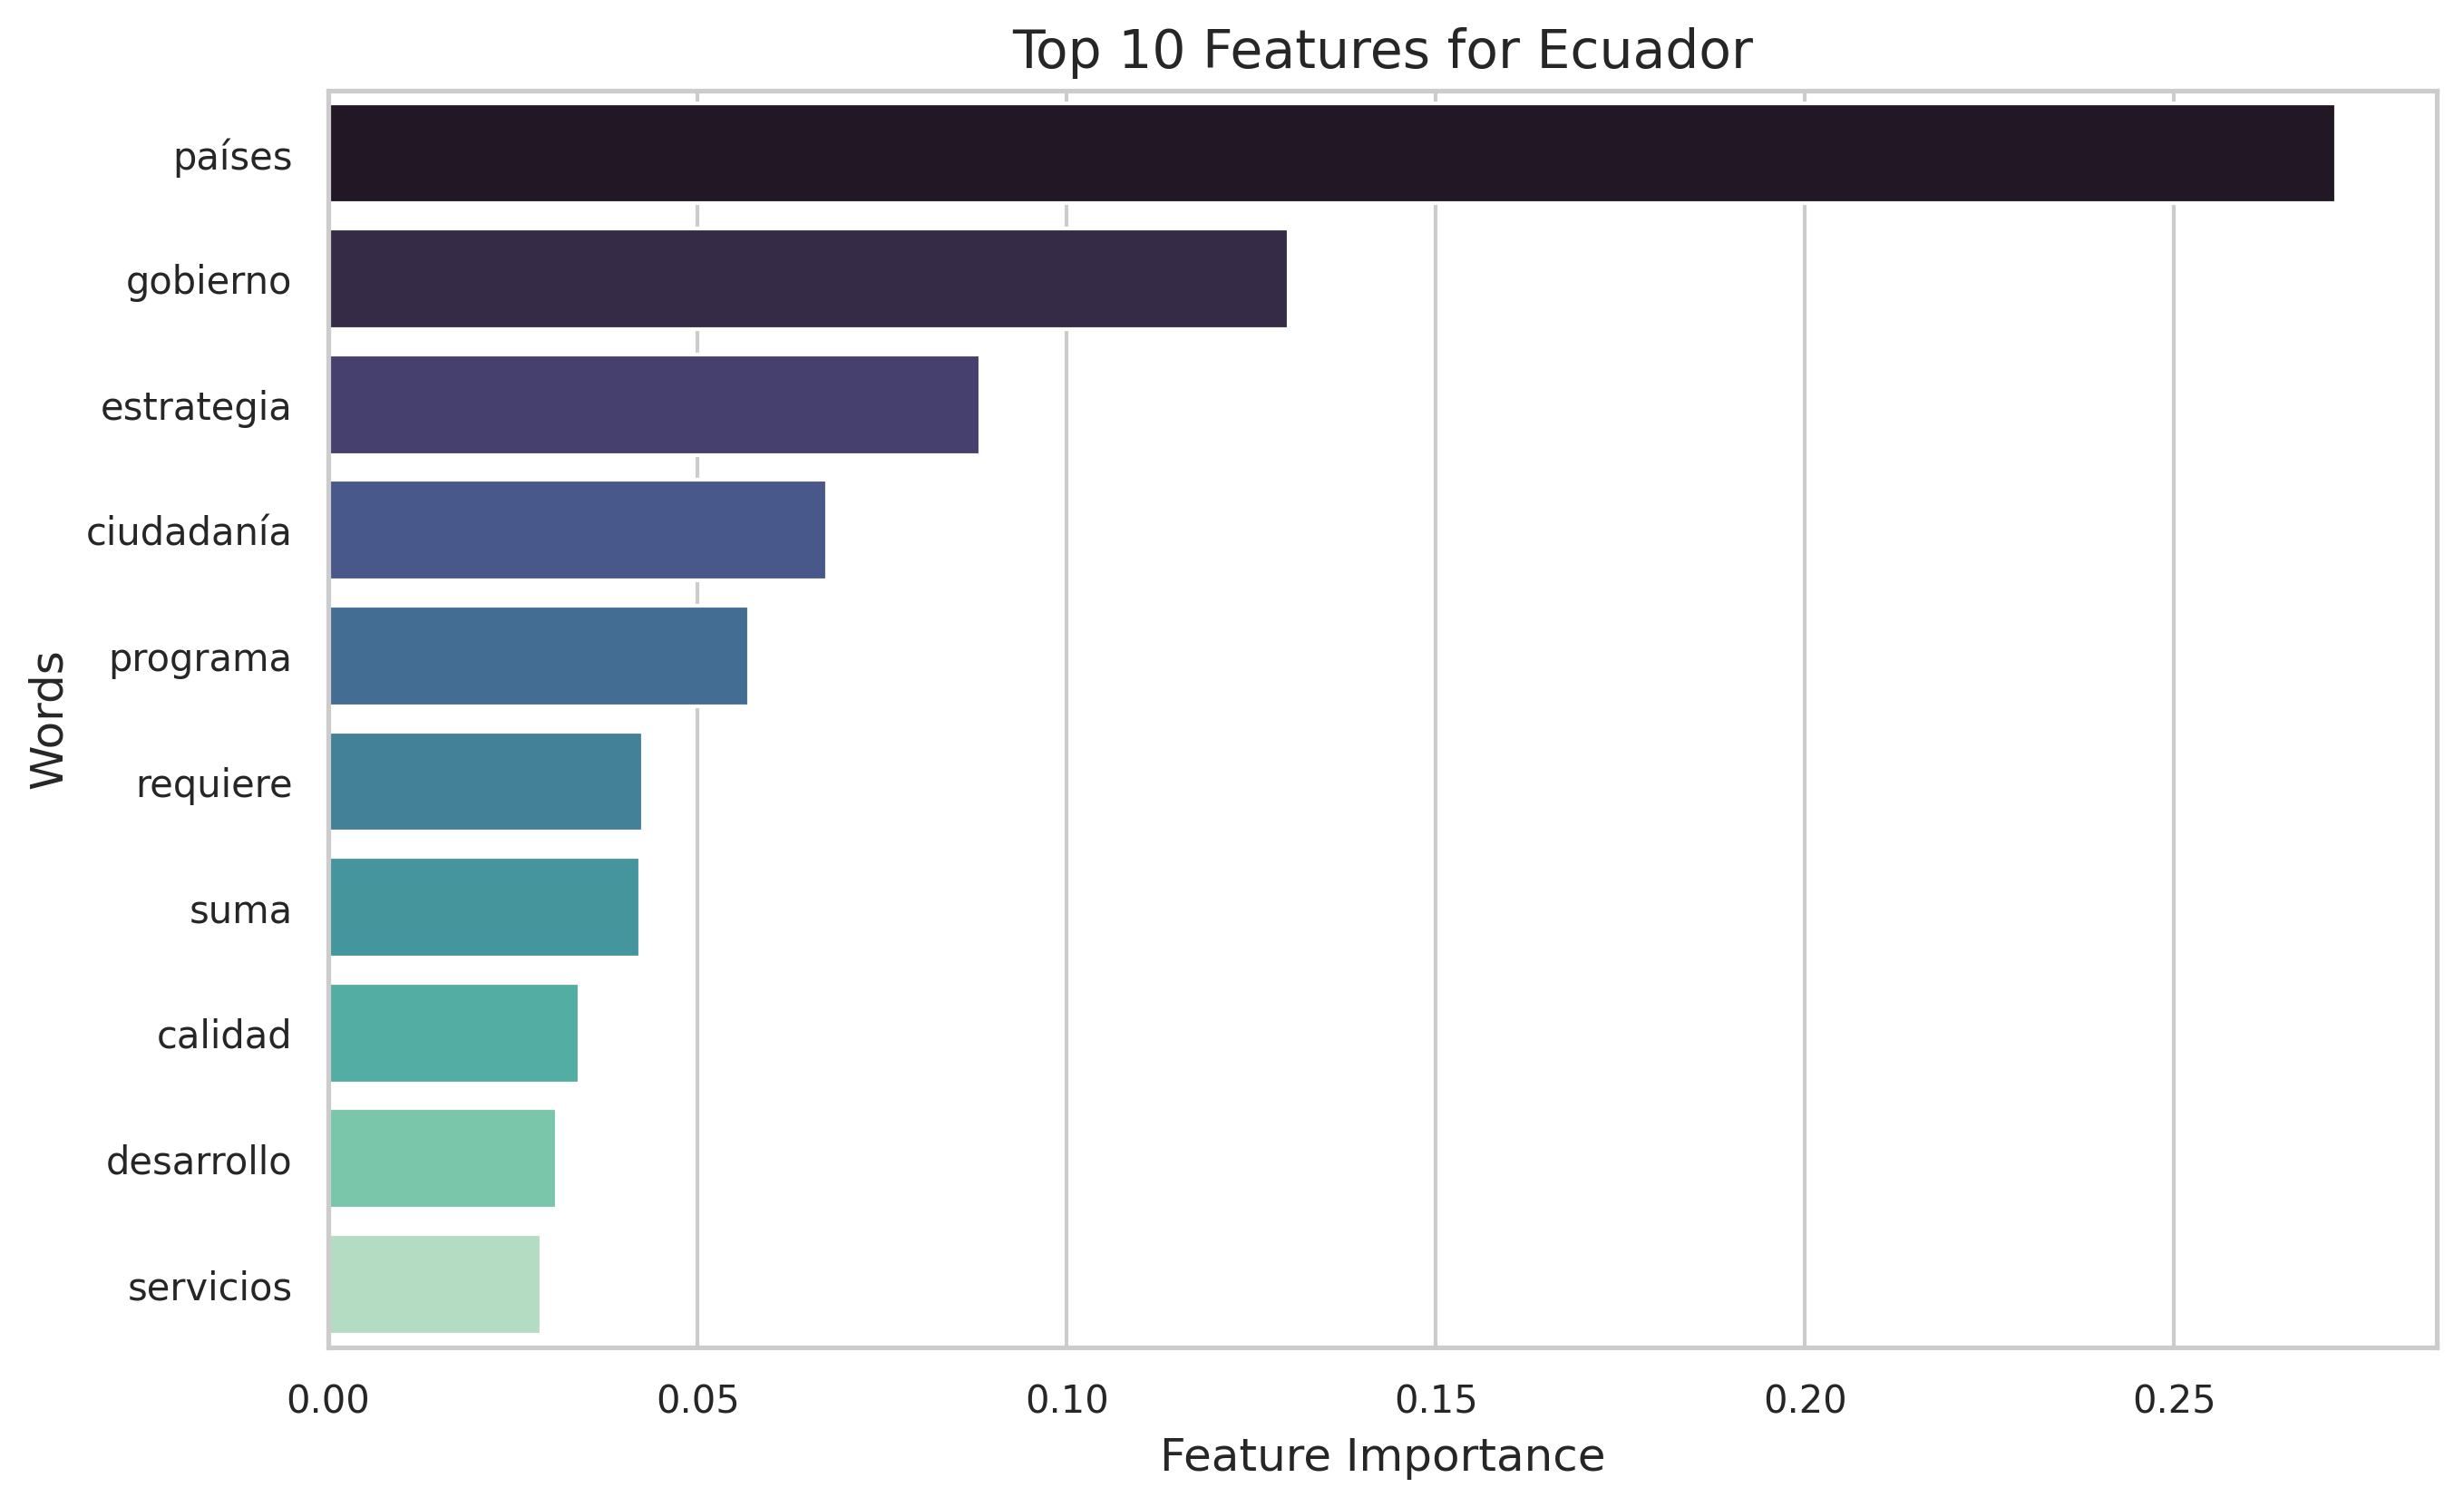
\includegraphics[width=0.8\textwidth]{/Users/sarabcidf/Desktop/ASDS/Dissertation/FinalScripts/CallanByCountry/Ecuador_feature_importance.png}
	\end{figure}
	\begin{figure}[H]
		\centering
		\caption{Error Rate for Ecuador Model}
		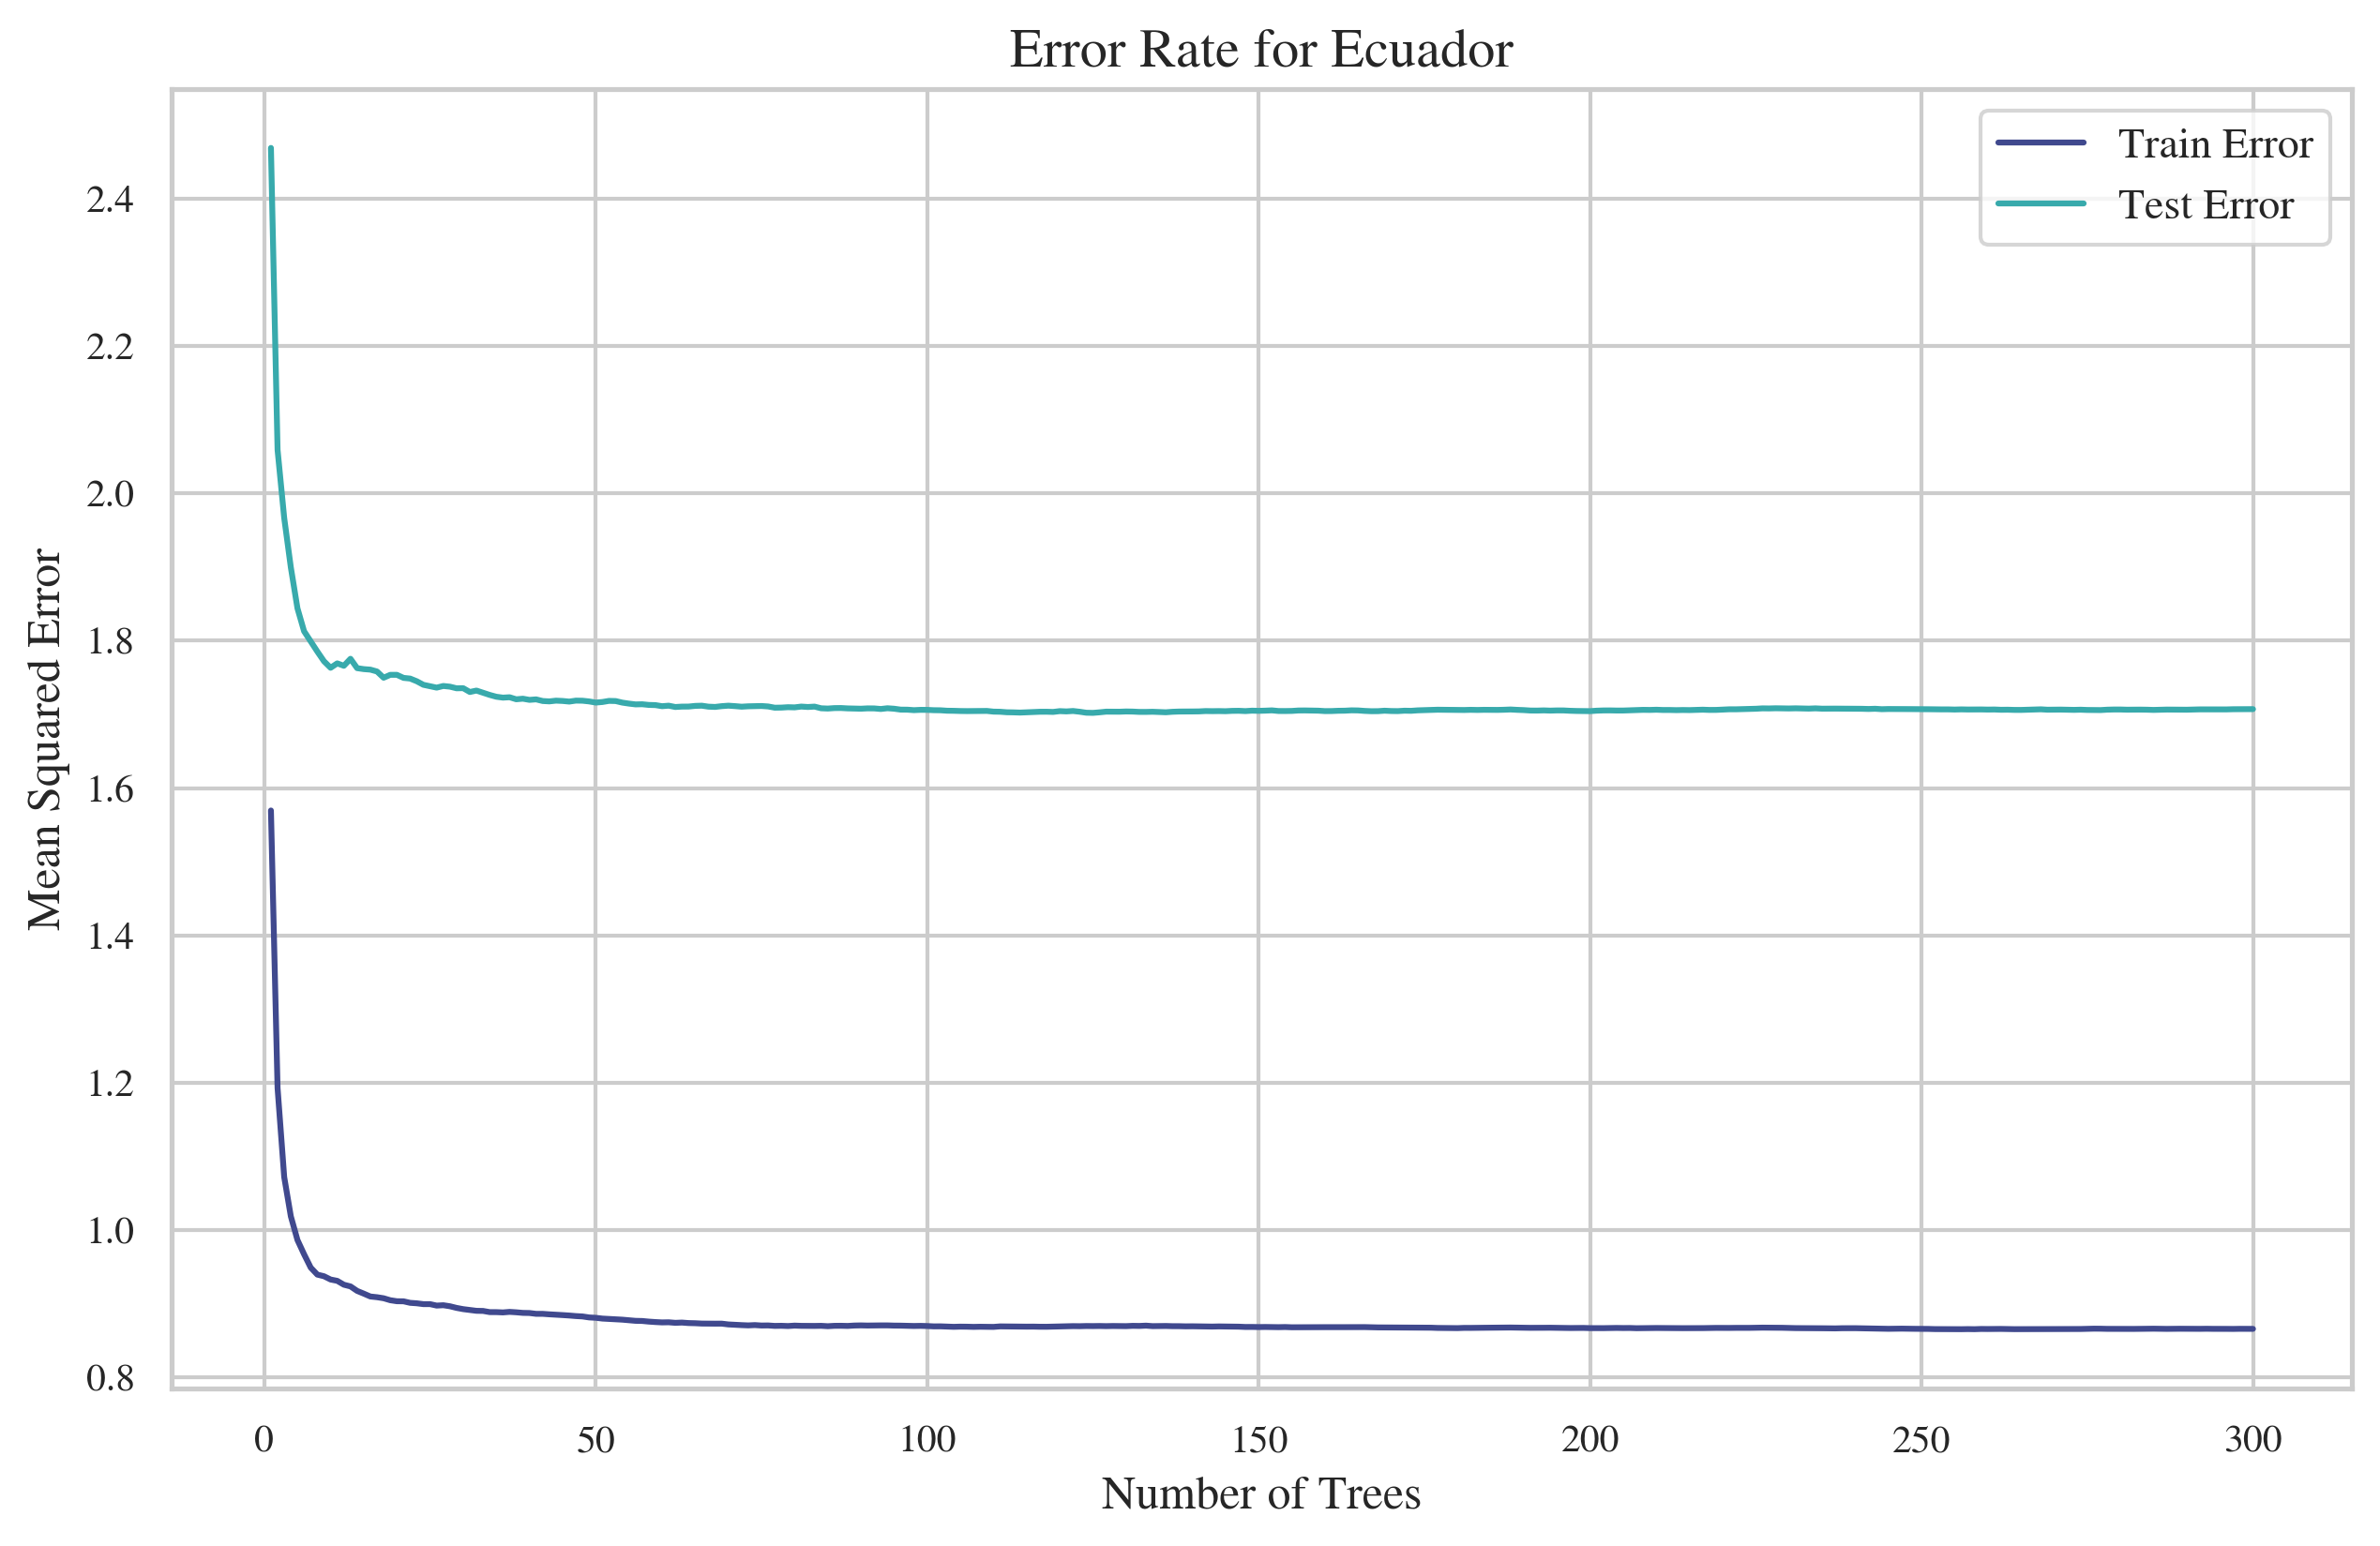
\includegraphics[width=0.8\textwidth]{/Users/sarabcidf/Desktop/ASDS/Dissertation/FinalScripts/CallanByCountry/Ecuador_error_rate.png}
	\end{figure}
	\begin{figure}[H]
		\centering
		\caption{Learning Curve for Ecuador Model}
		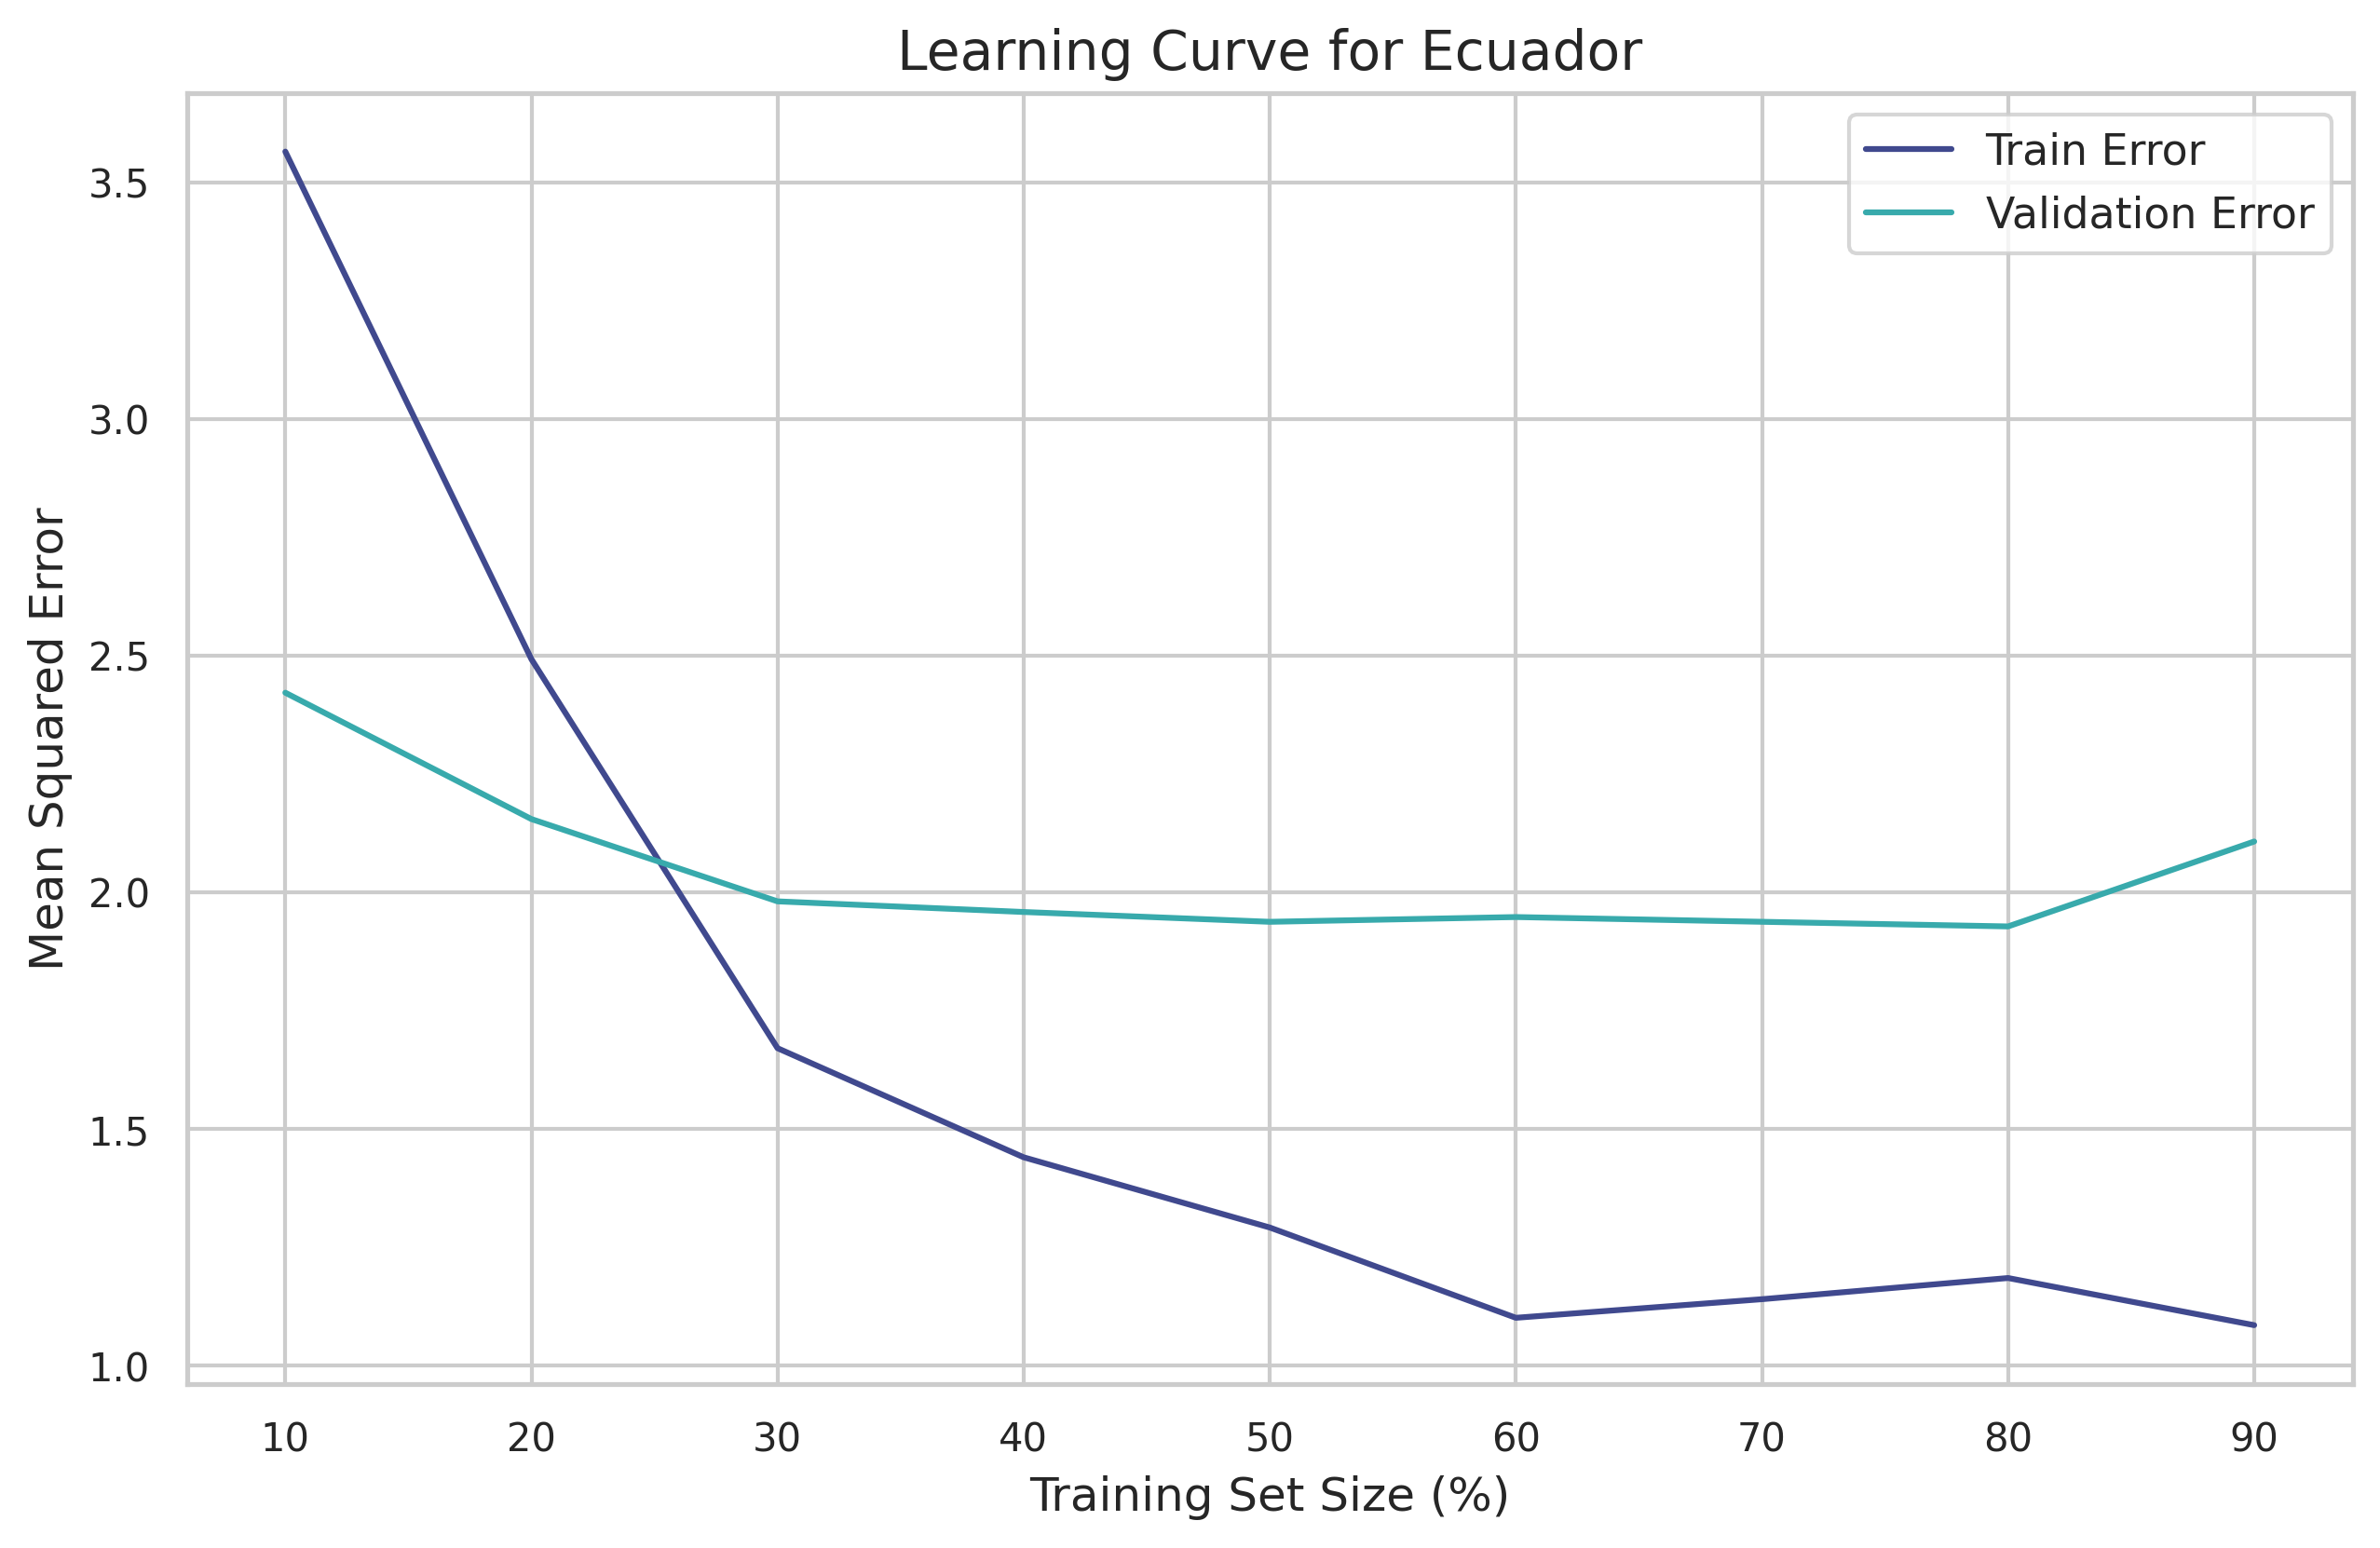
\includegraphics[width=0.8\textwidth]{/Users/sarabcidf/Desktop/ASDS/Dissertation/FinalScripts/CallanByCountry/Ecuador_learning_curve.png}
	\end{figure}
	
	\newpage
	
	\subsection{Mexico}
	\begin{figure}[H]
		\centering
		\caption{Feature Importance for Mexico Model}
		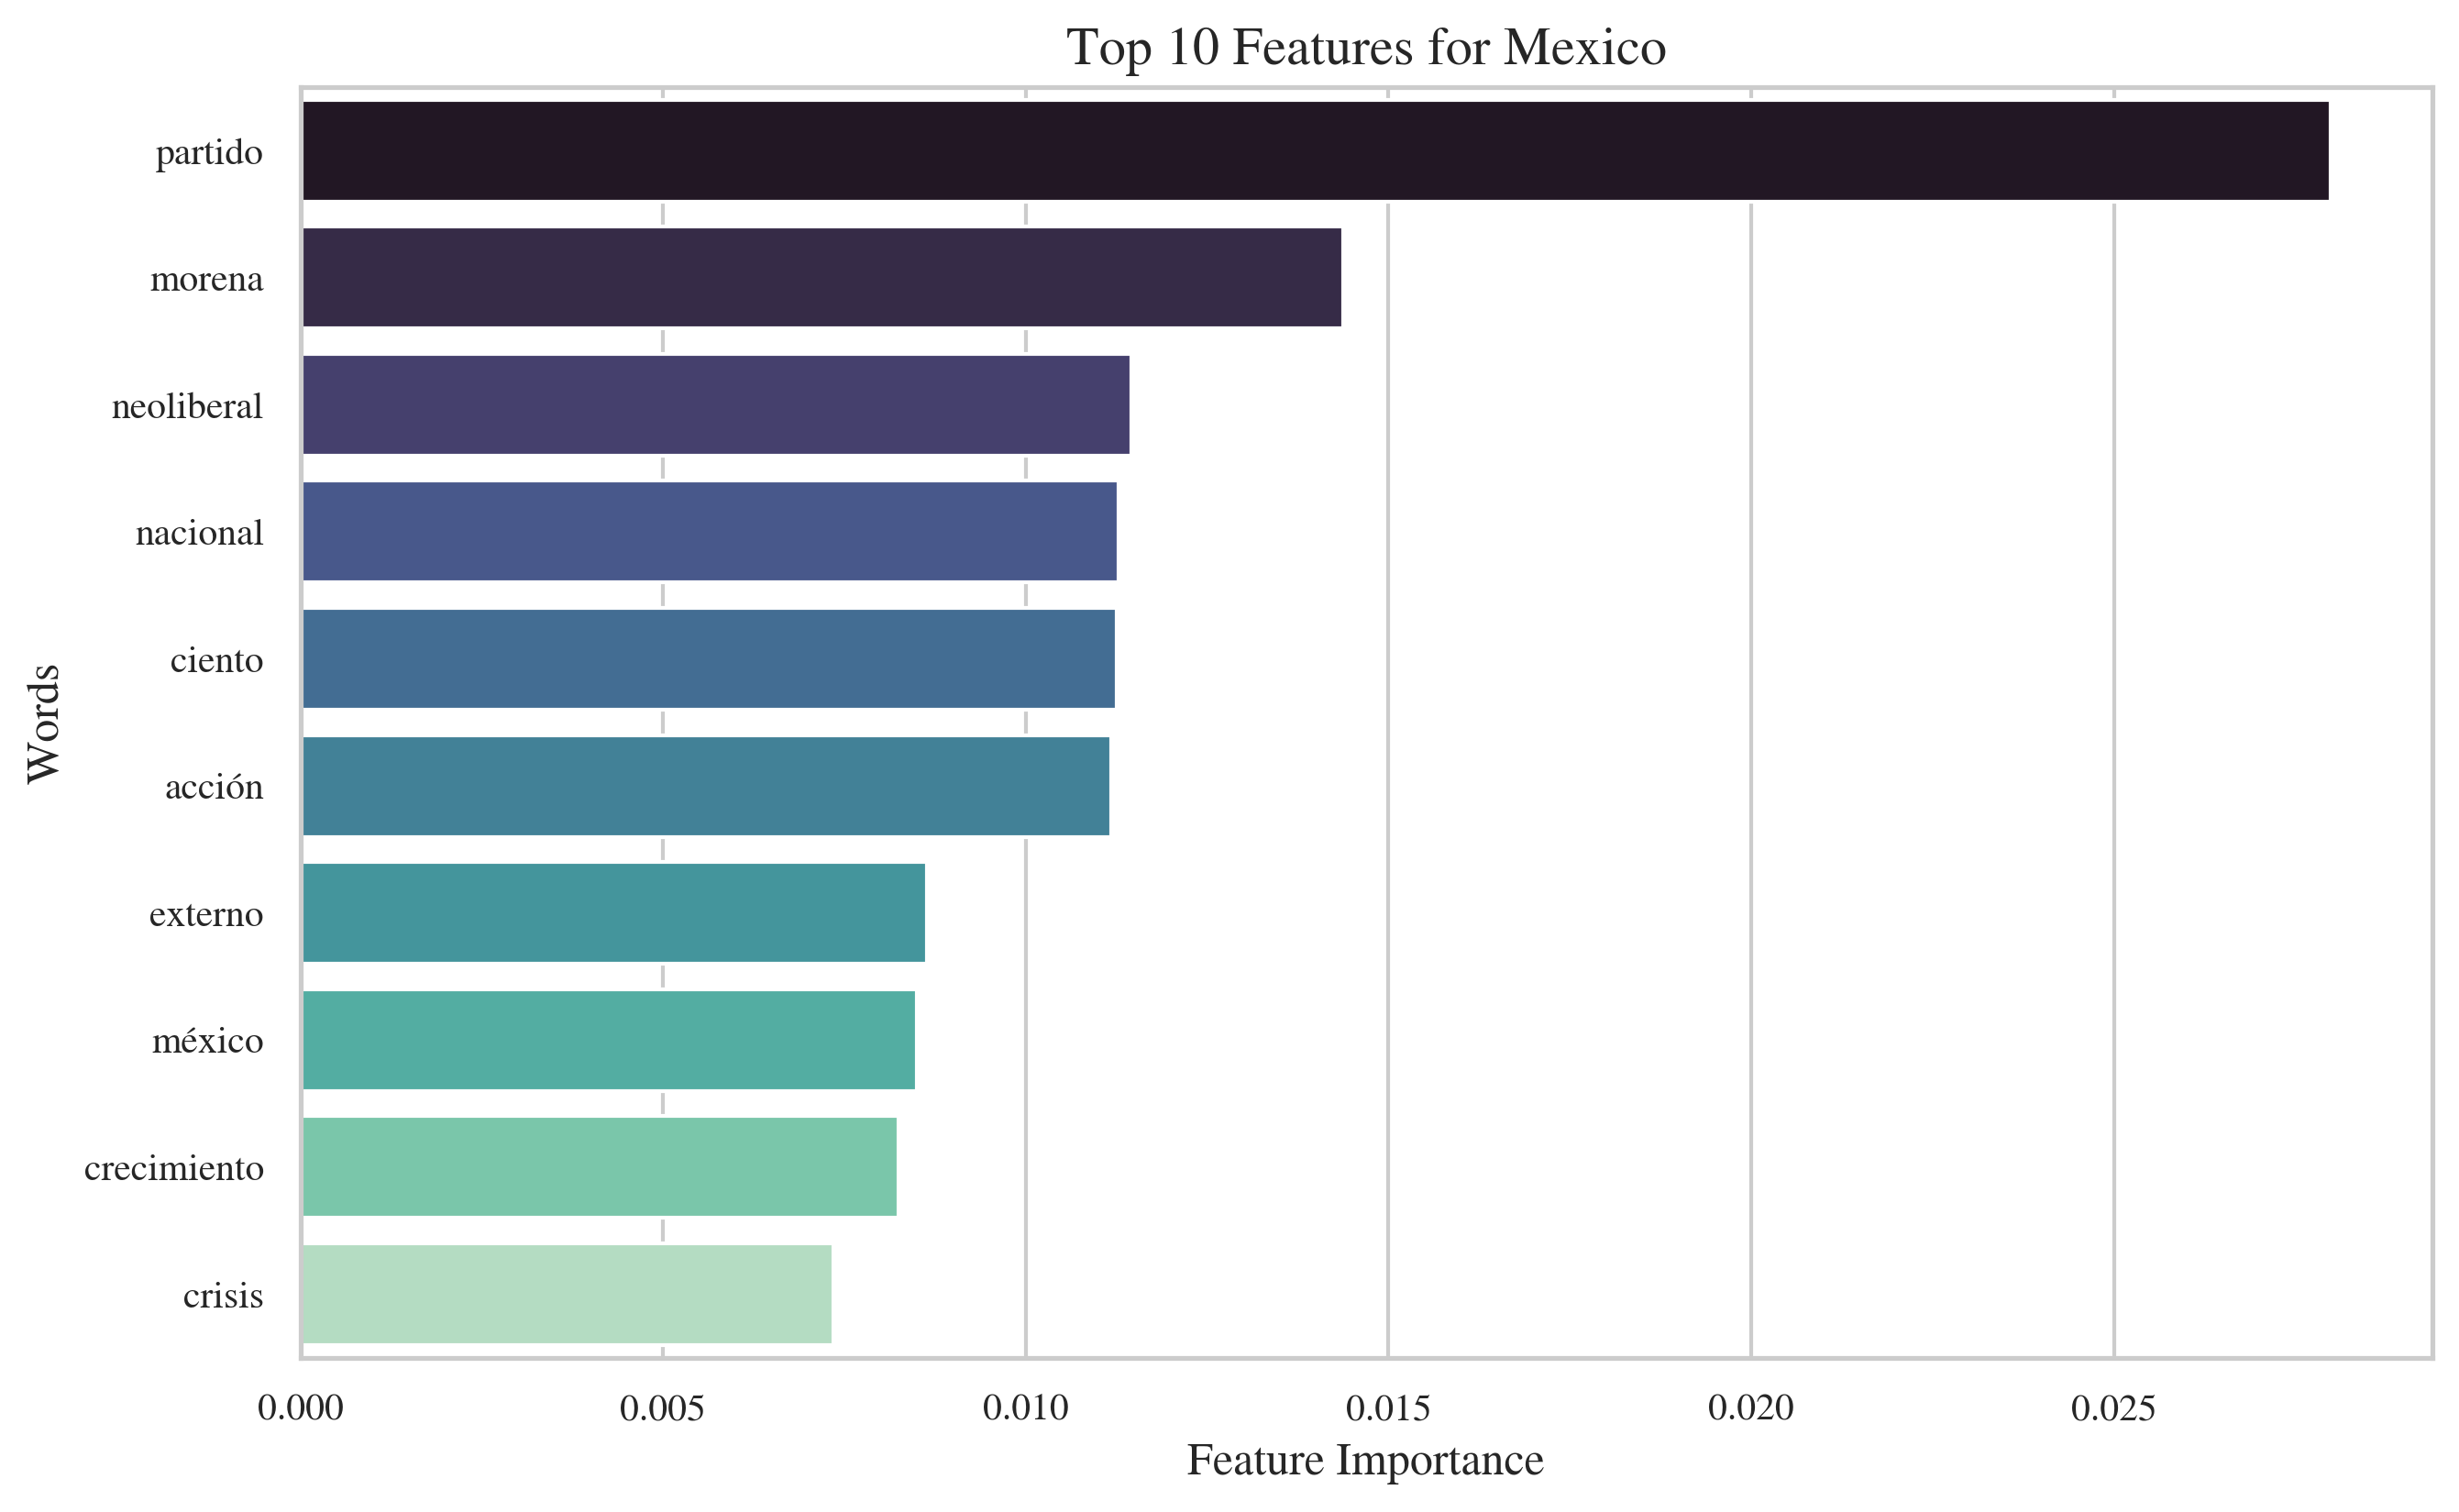
\includegraphics[width=0.8\textwidth]{/Users/sarabcidf/Desktop/ASDS/Dissertation/FinalScripts/CallanByCountry/Mexico_feature_importance.png}
	\end{figure}
	\begin{figure}[H]
		\centering
		\caption{Error Rate for Mexico Model}
		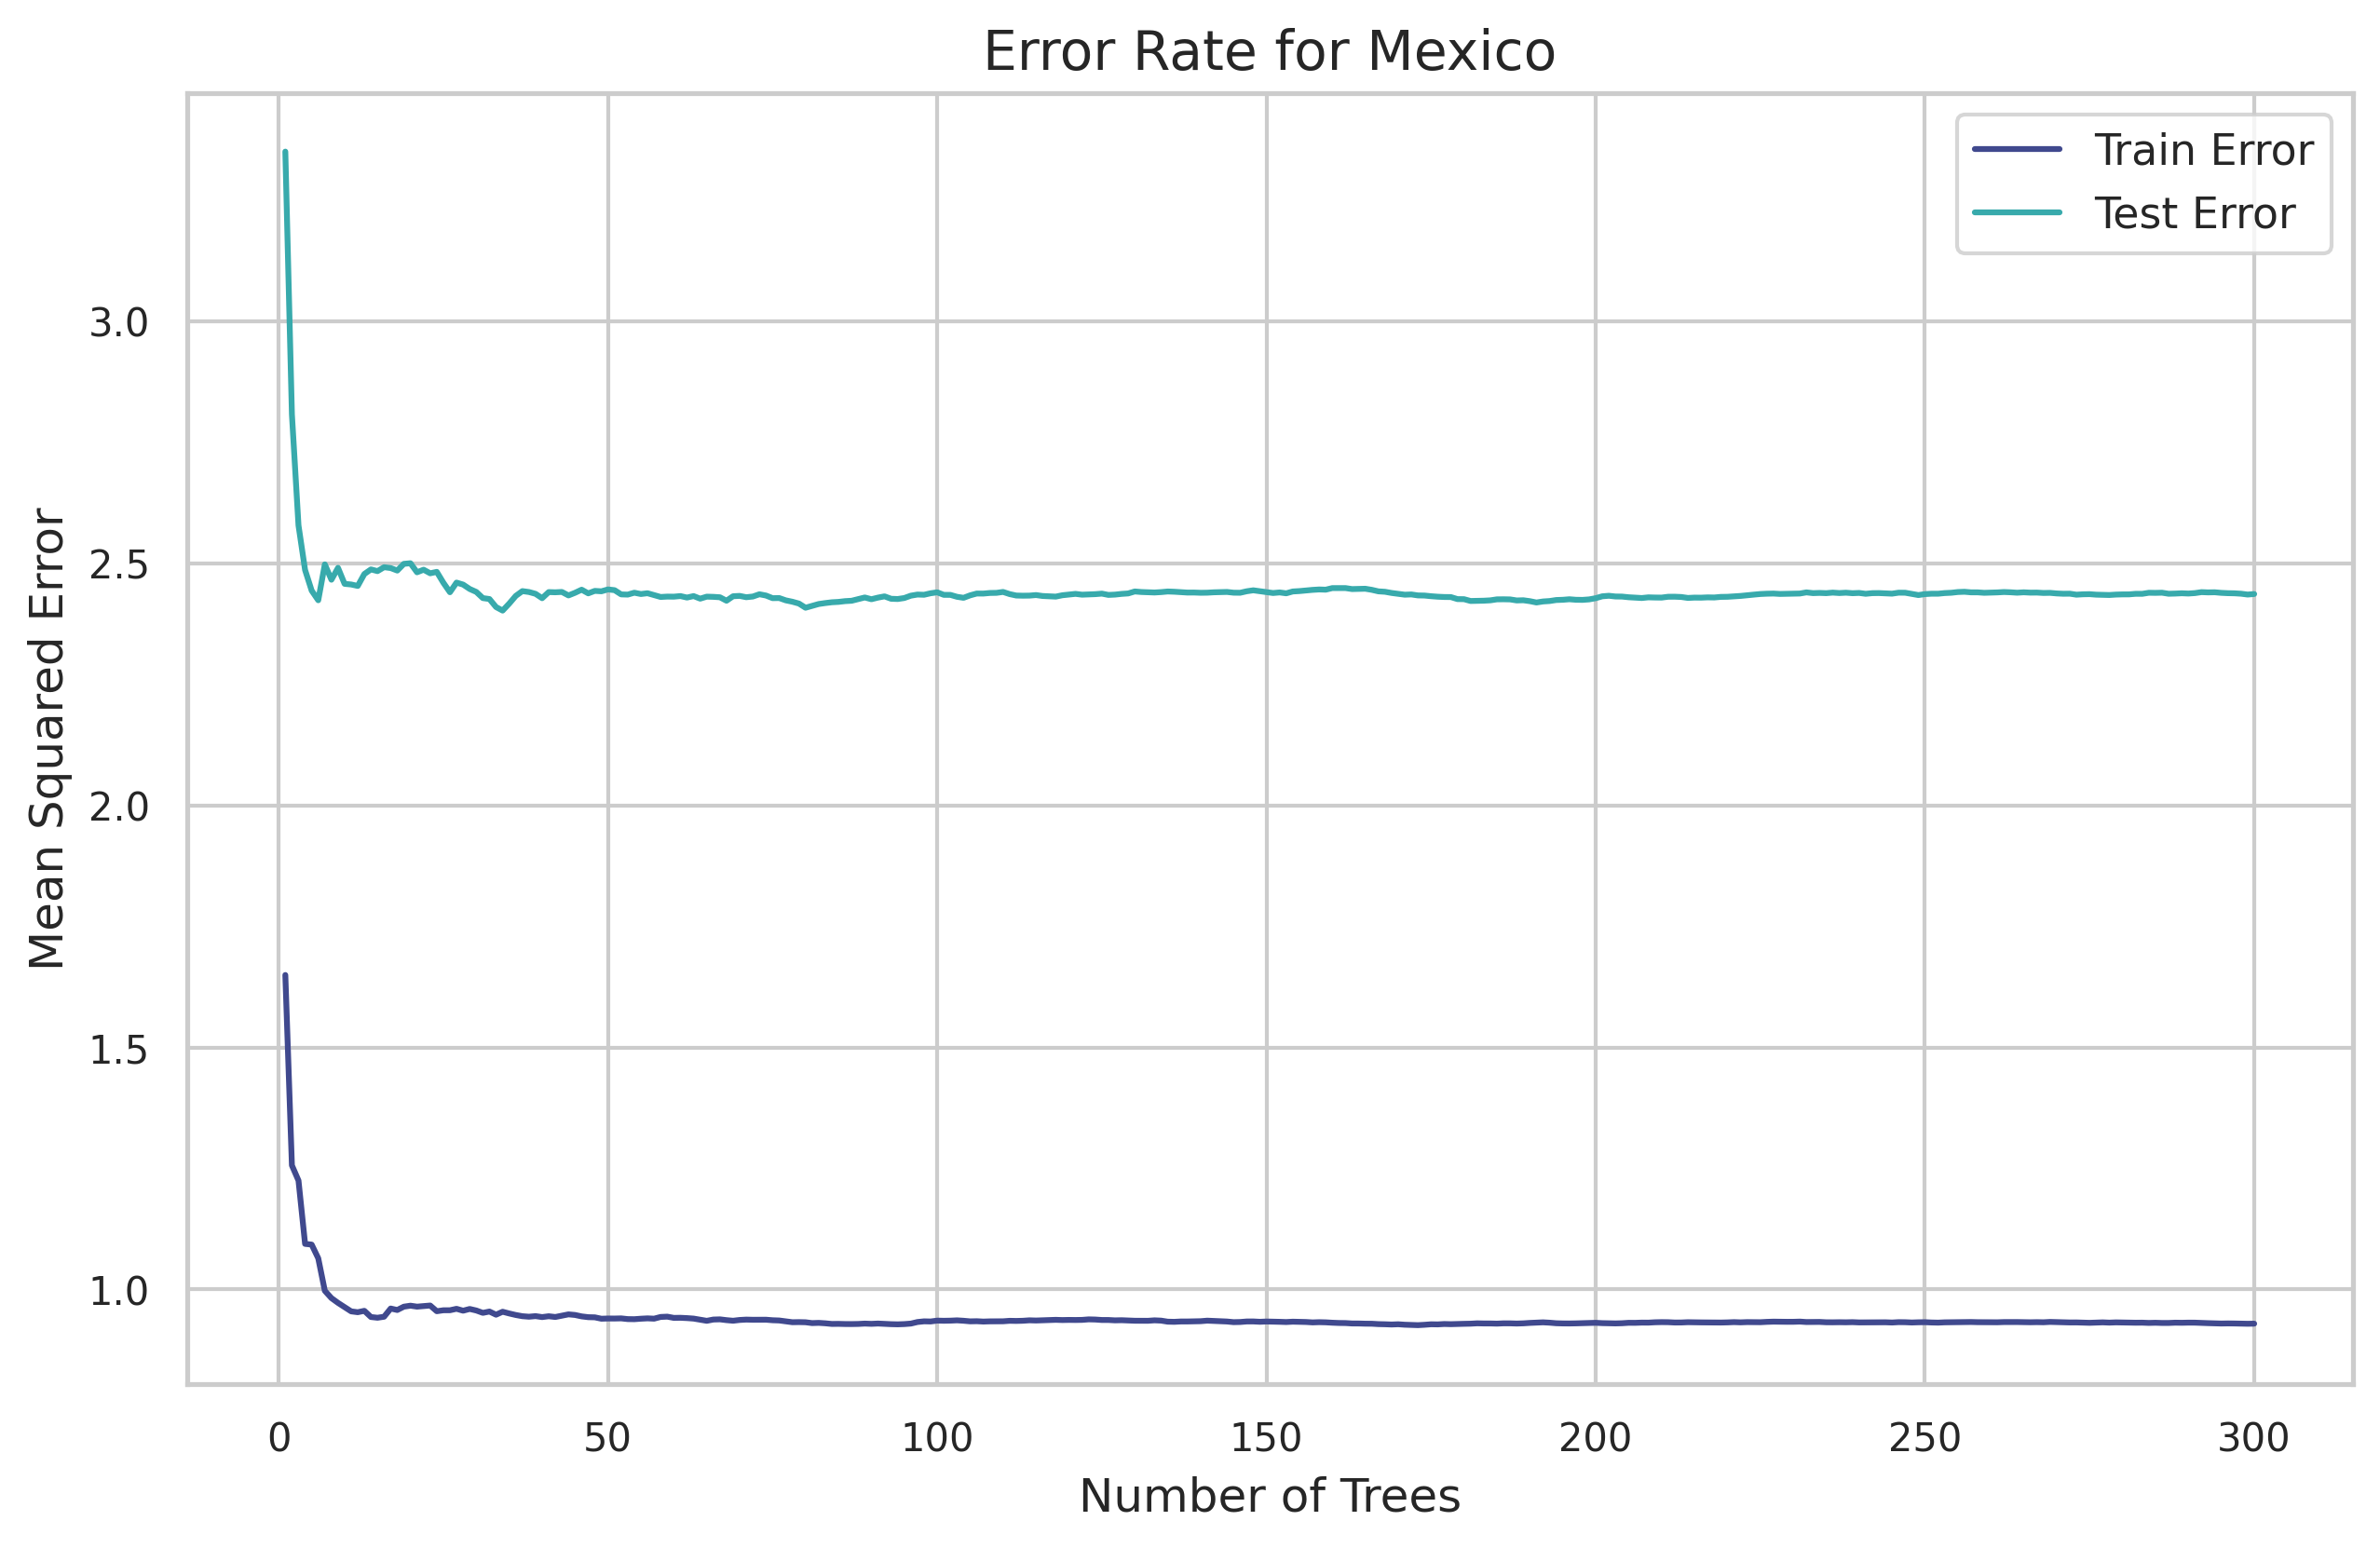
\includegraphics[width=0.8\textwidth]{/Users/sarabcidf/Desktop/ASDS/Dissertation/FinalScripts/CallanByCountry/Mexico_error_rate.png}
	\end{figure}
	\begin{figure}[H]
		\centering
		\caption{Learning Curve for Mexico Model}
		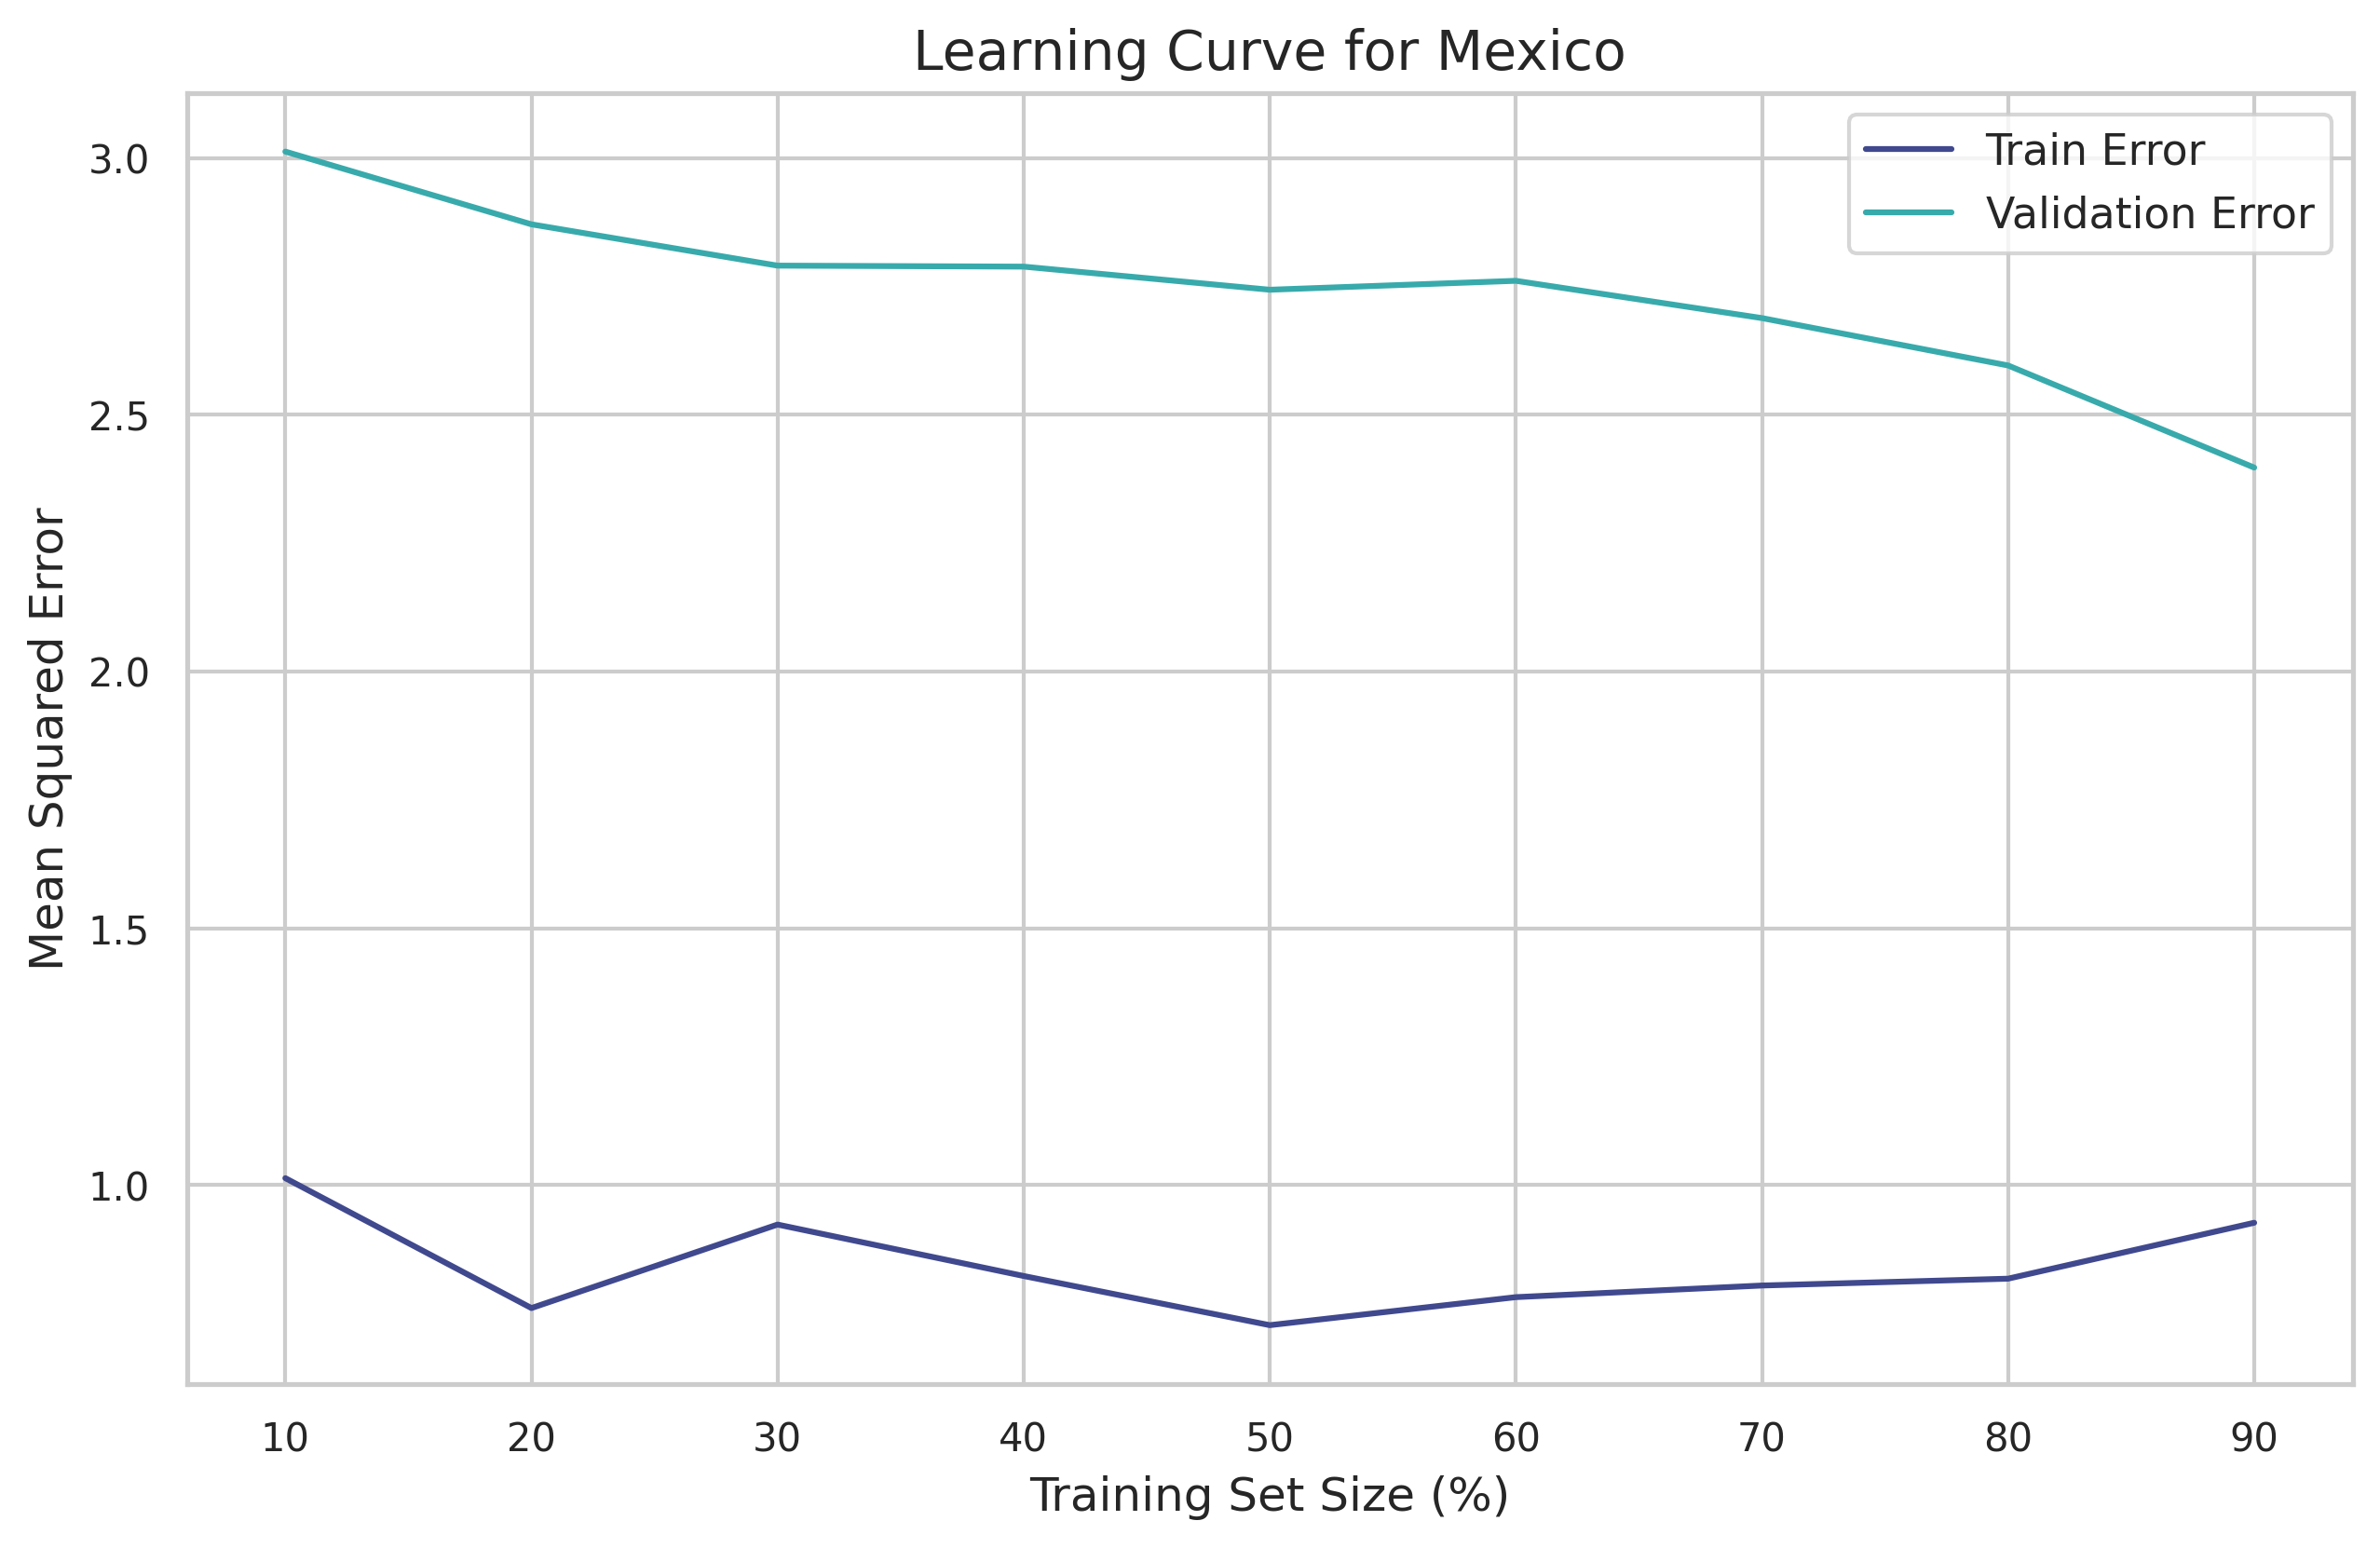
\includegraphics[width=0.8\textwidth]{/Users/sarabcidf/Desktop/ASDS/Dissertation/FinalScripts/CallanByCountry/Mexico_learning_curve.png}
	\end{figure}

	\newpage
	
	\subsection{Panama}
	\begin{figure}[H]
		\centering
		\caption{Feature Importance for Panama Model}
		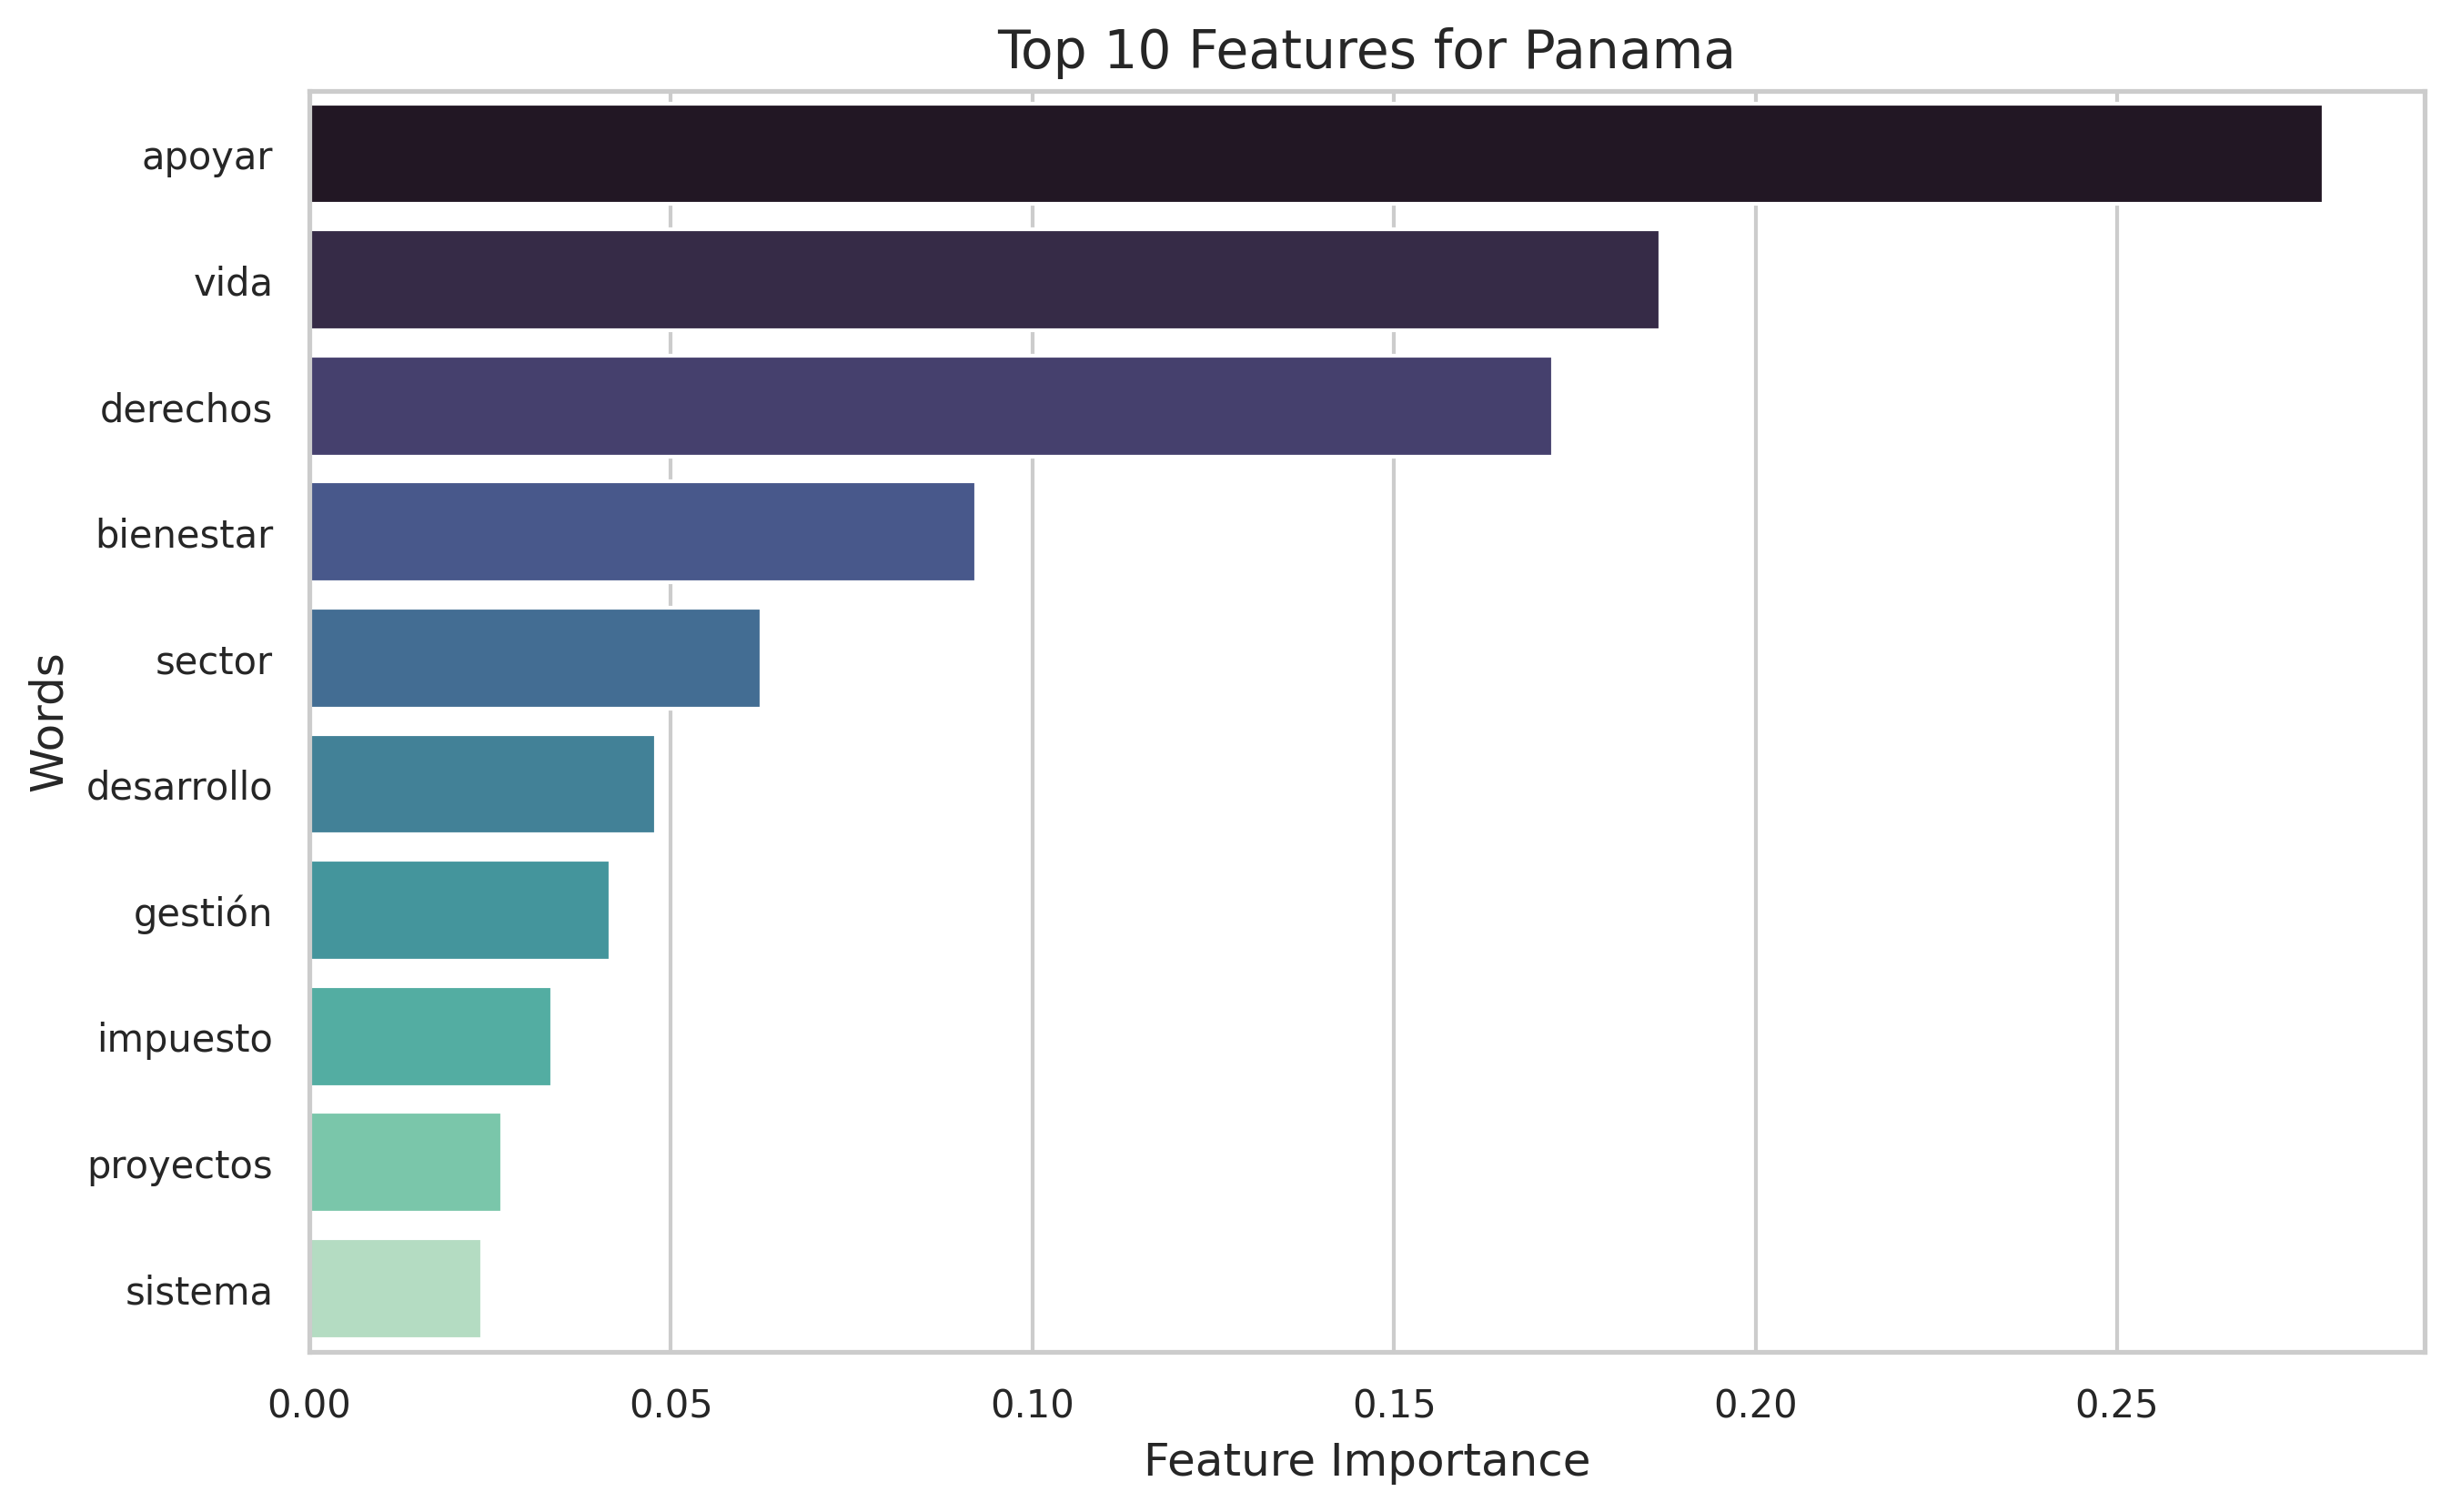
\includegraphics[width=0.8\textwidth]{/Users/sarabcidf/Desktop/ASDS/Dissertation/FinalScripts/CallanByCountry/Panama_feature_importance.png}
	\end{figure}
	\begin{figure}[H]
		\centering
		\caption{Error Rate for Panama Model}
		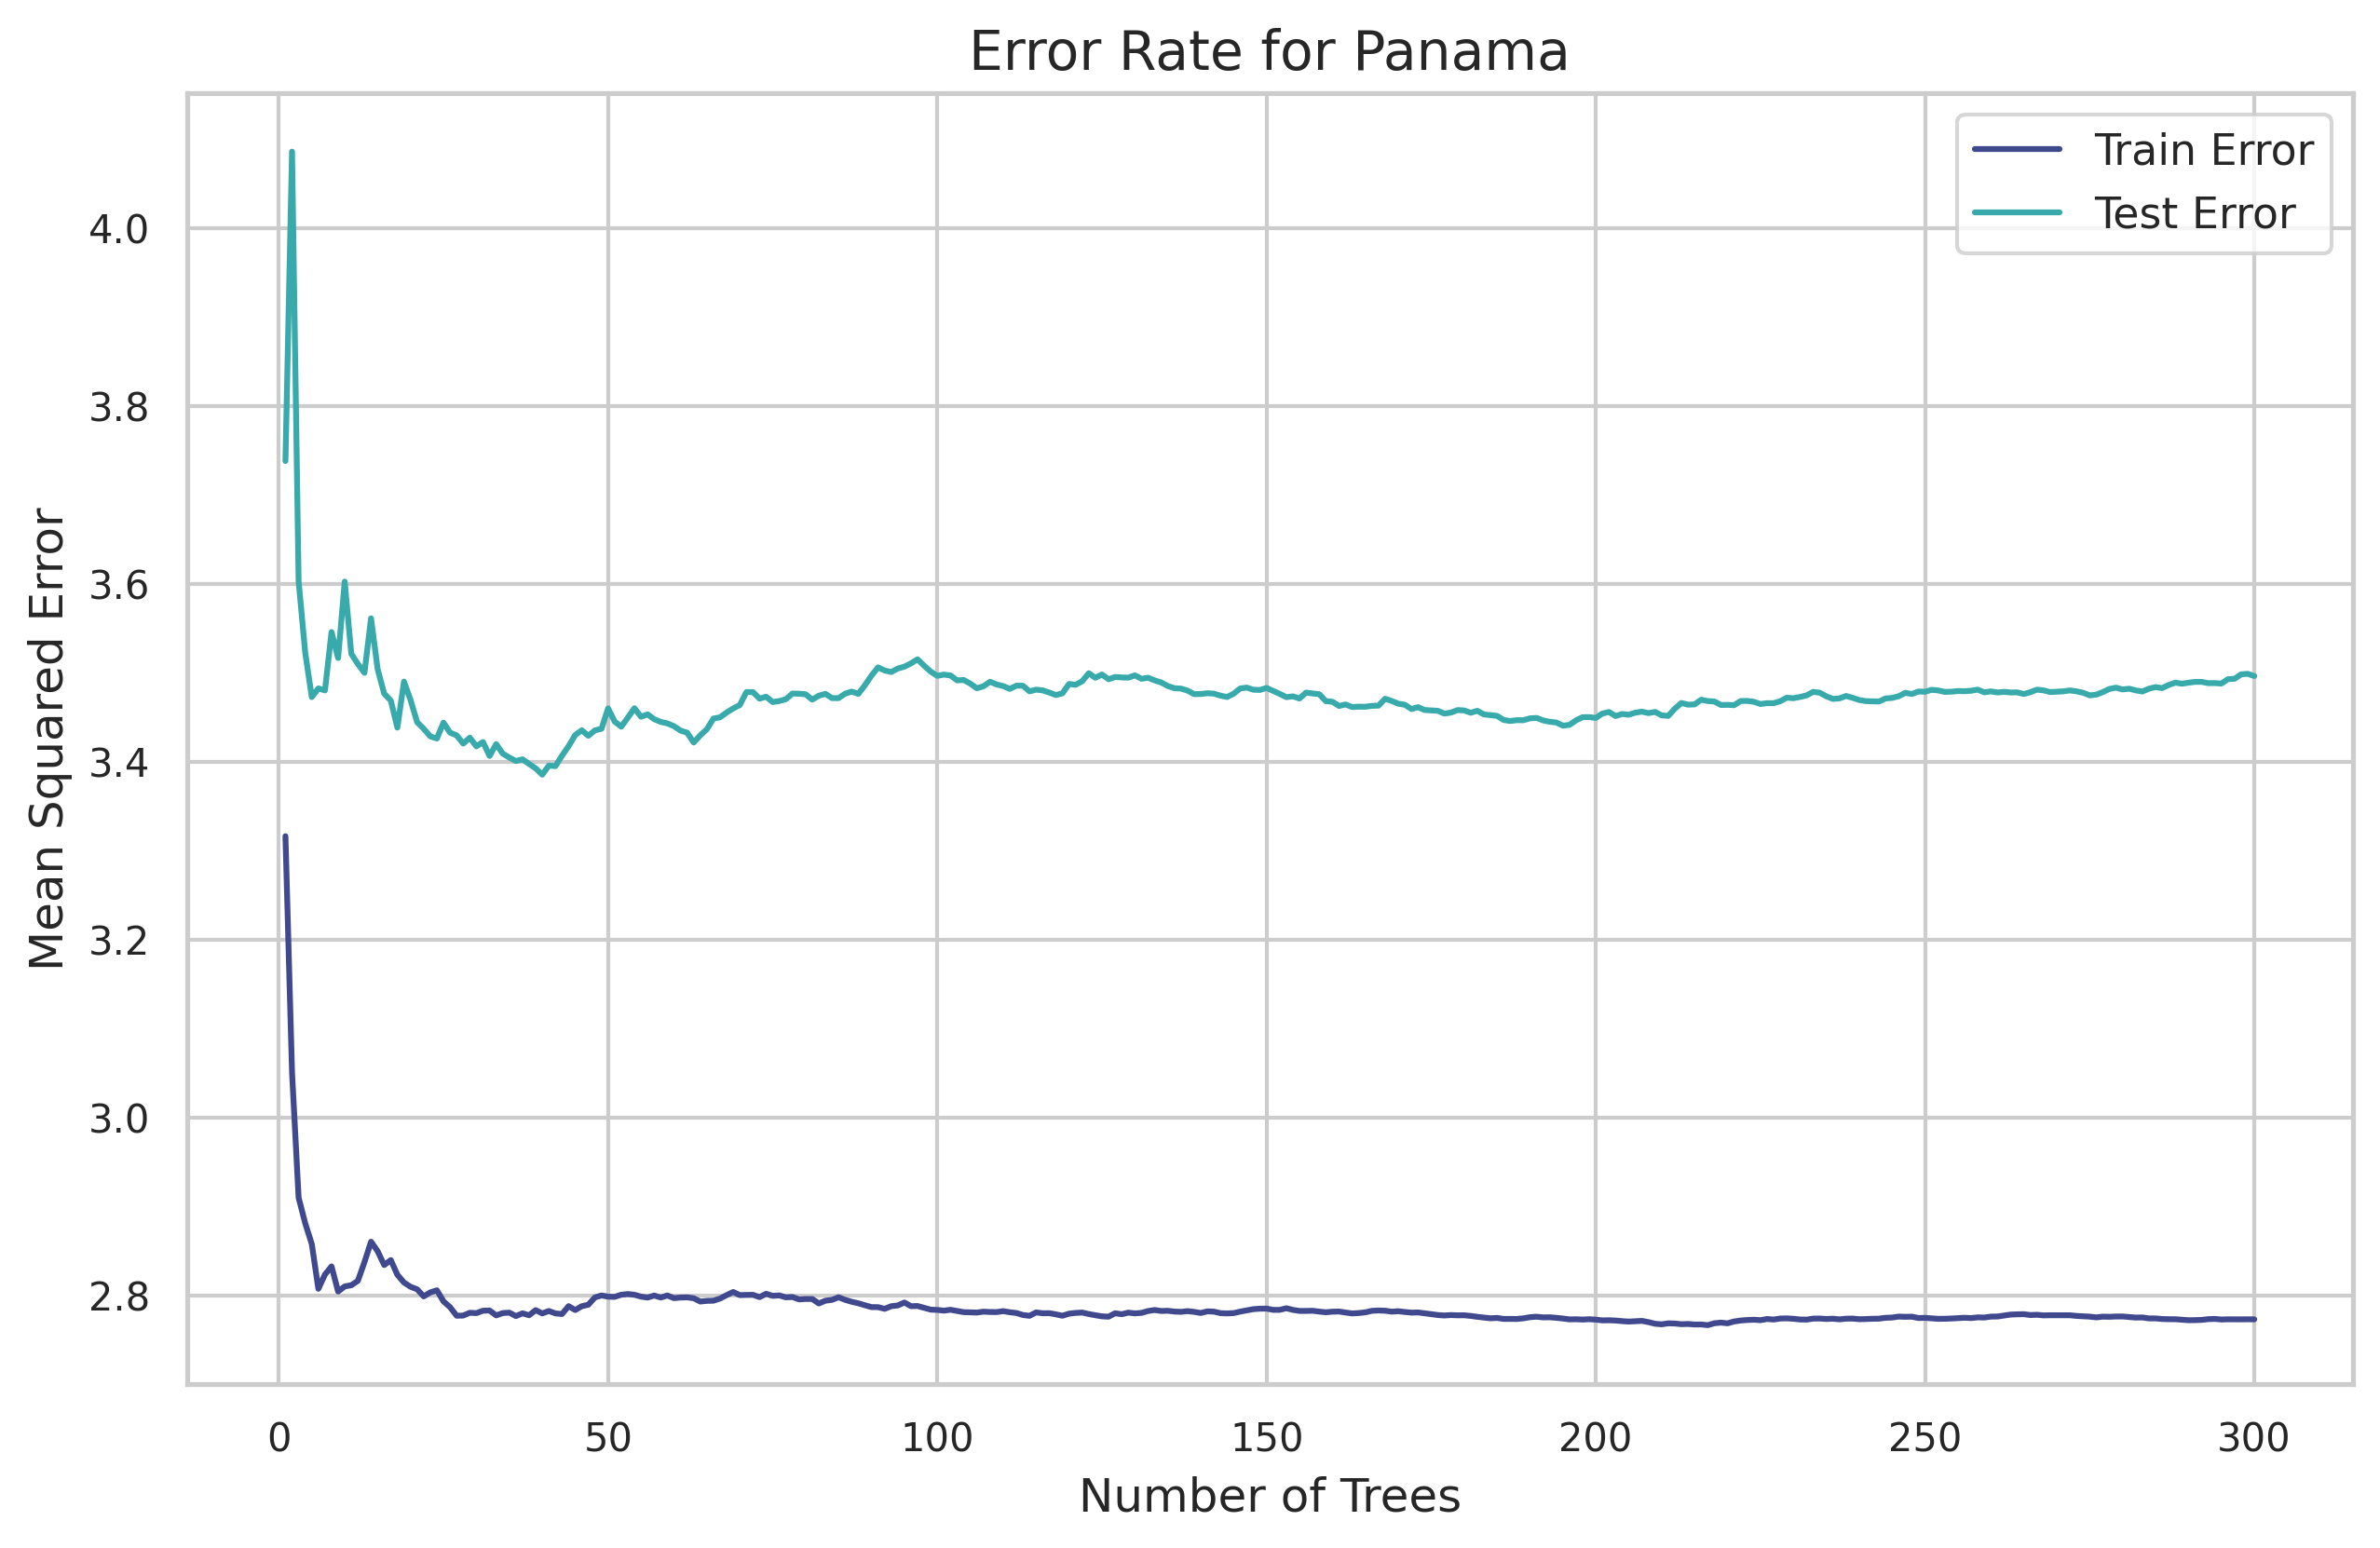
\includegraphics[width=0.8\textwidth]{/Users/sarabcidf/Desktop/ASDS/Dissertation/FinalScripts/CallanByCountry/Panama_error_rate.png}
	\end{figure}
	\begin{figure}[H]
		\centering
		\caption{Learning Curve for Panama Model}
		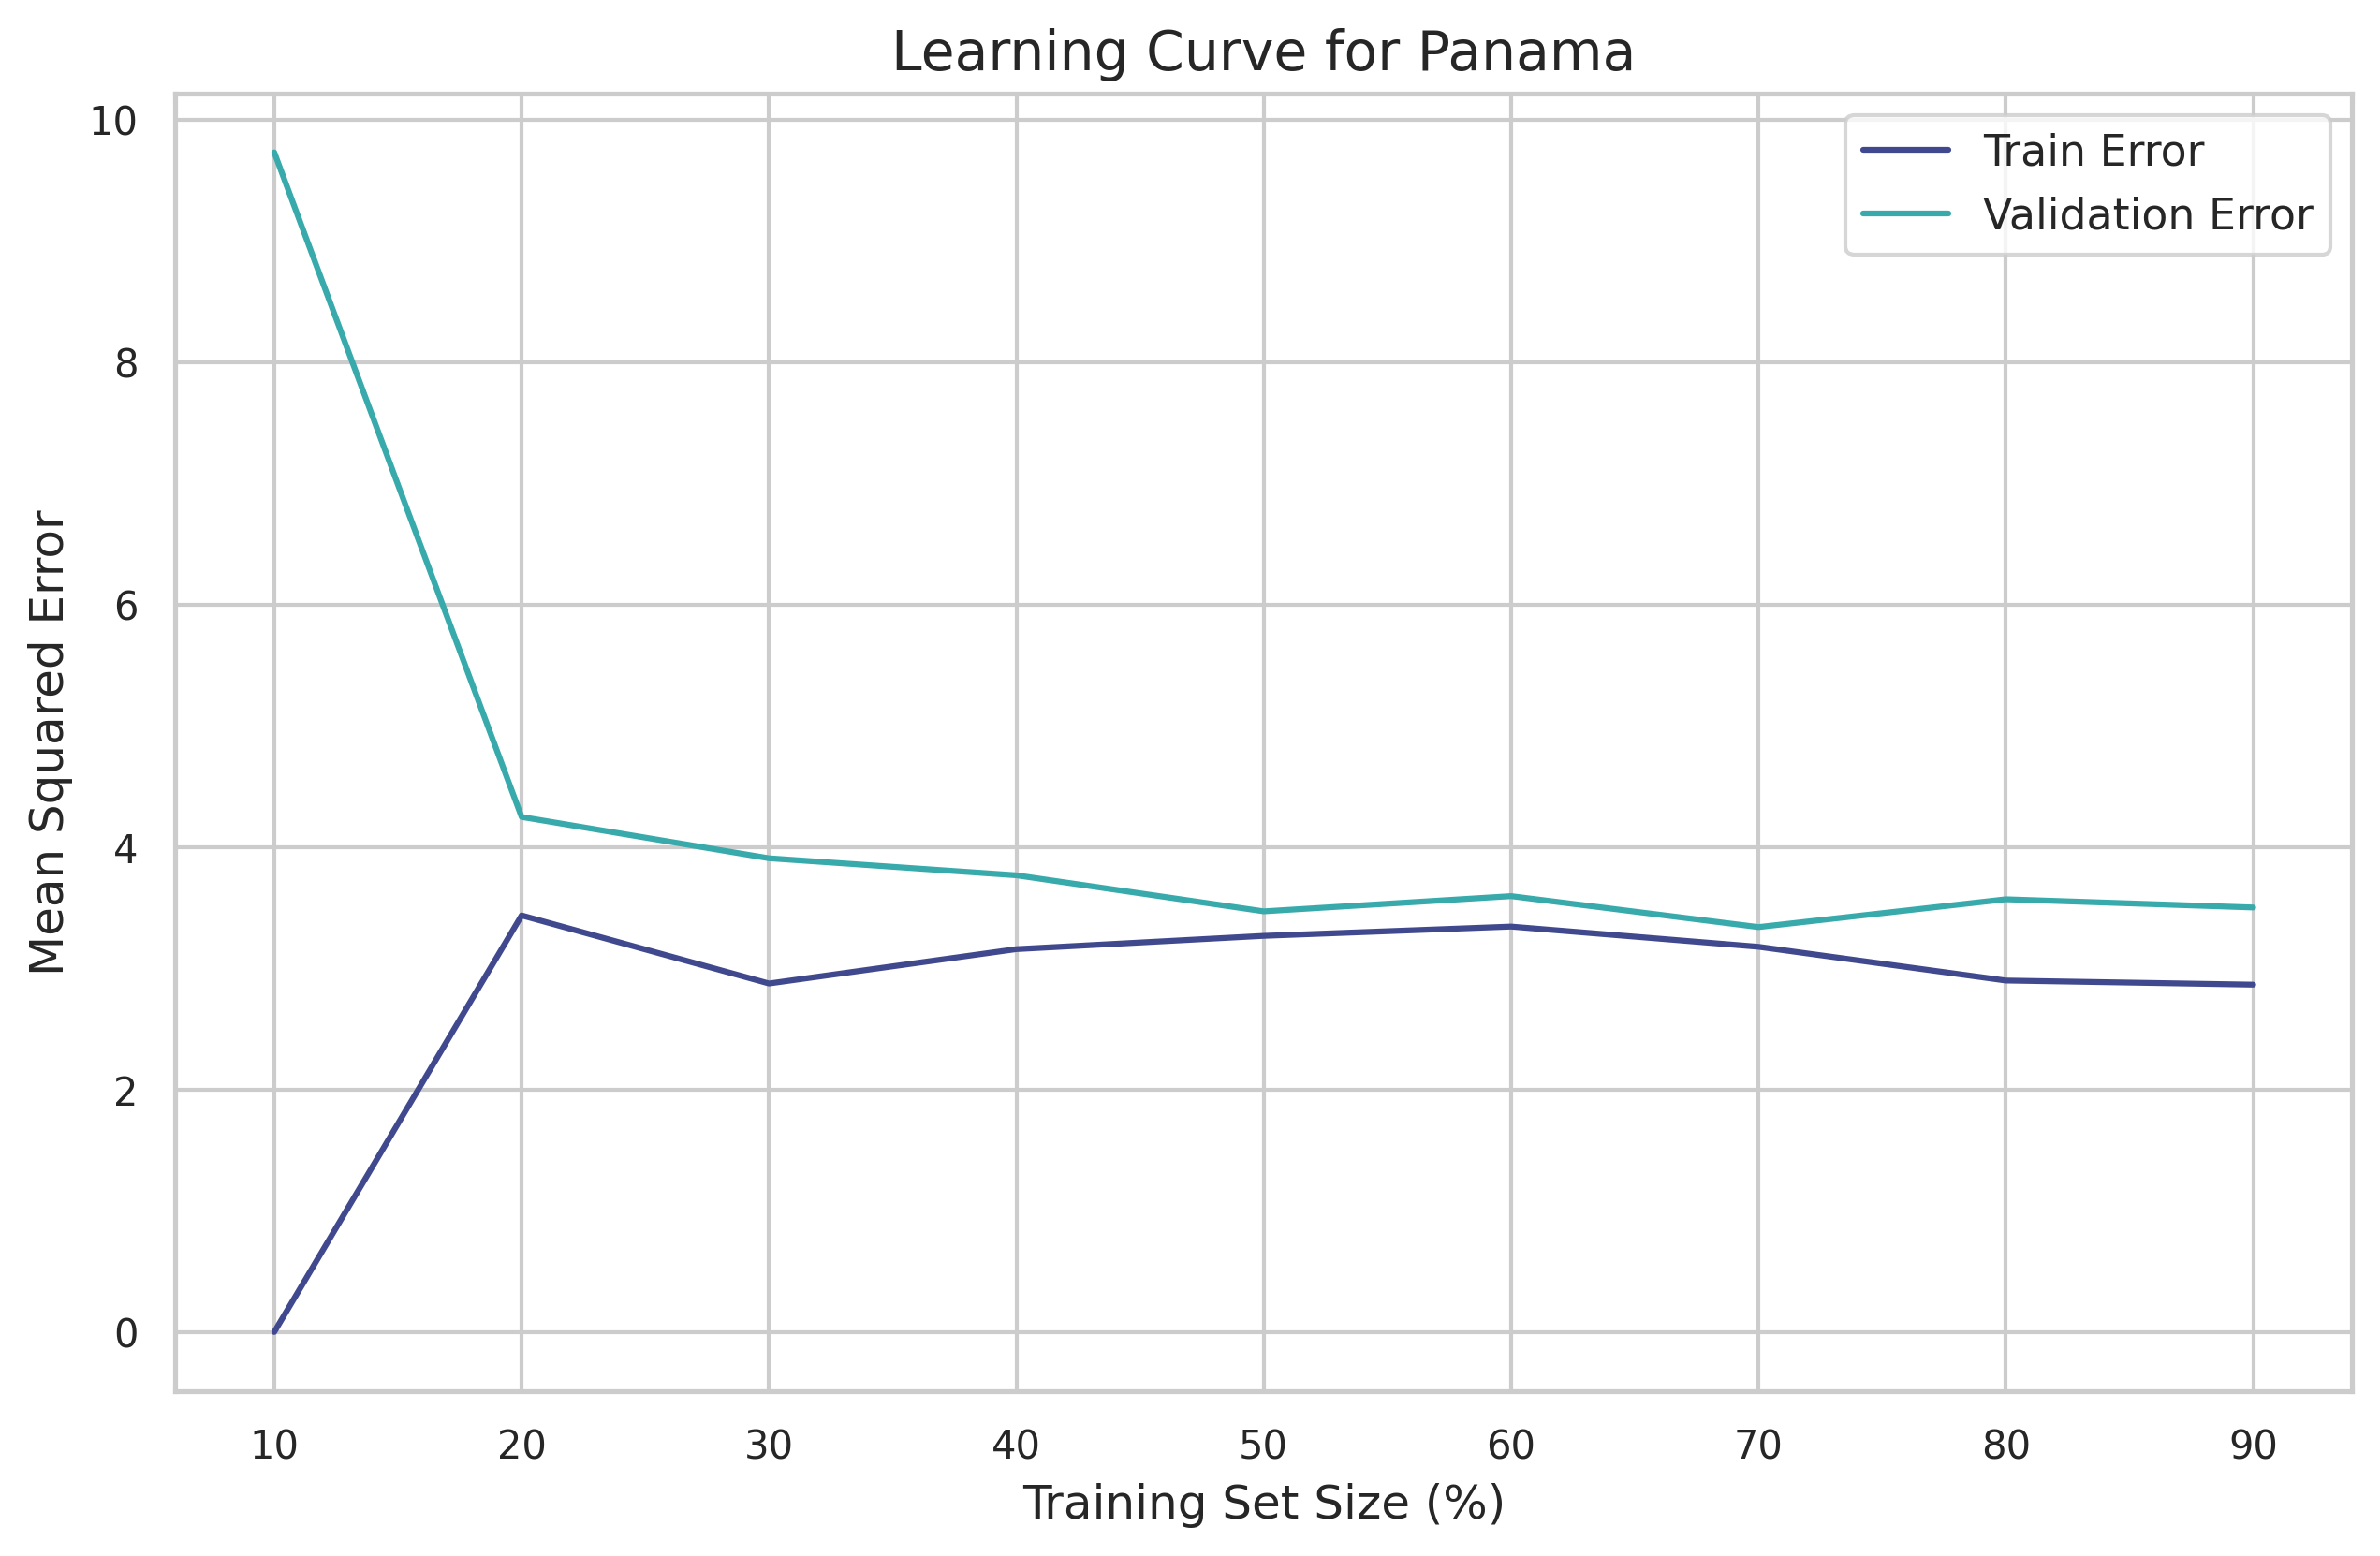
\includegraphics[width=0.8\textwidth]{/Users/sarabcidf/Desktop/ASDS/Dissertation/FinalScripts/CallanByCountry/Panama_learning_curve.png}
	\end{figure}
	
	\newpage
	
	\subsection{Peru}
	\begin{figure}[H]
		\centering
		\caption{Feature Importance for Peru Model}
		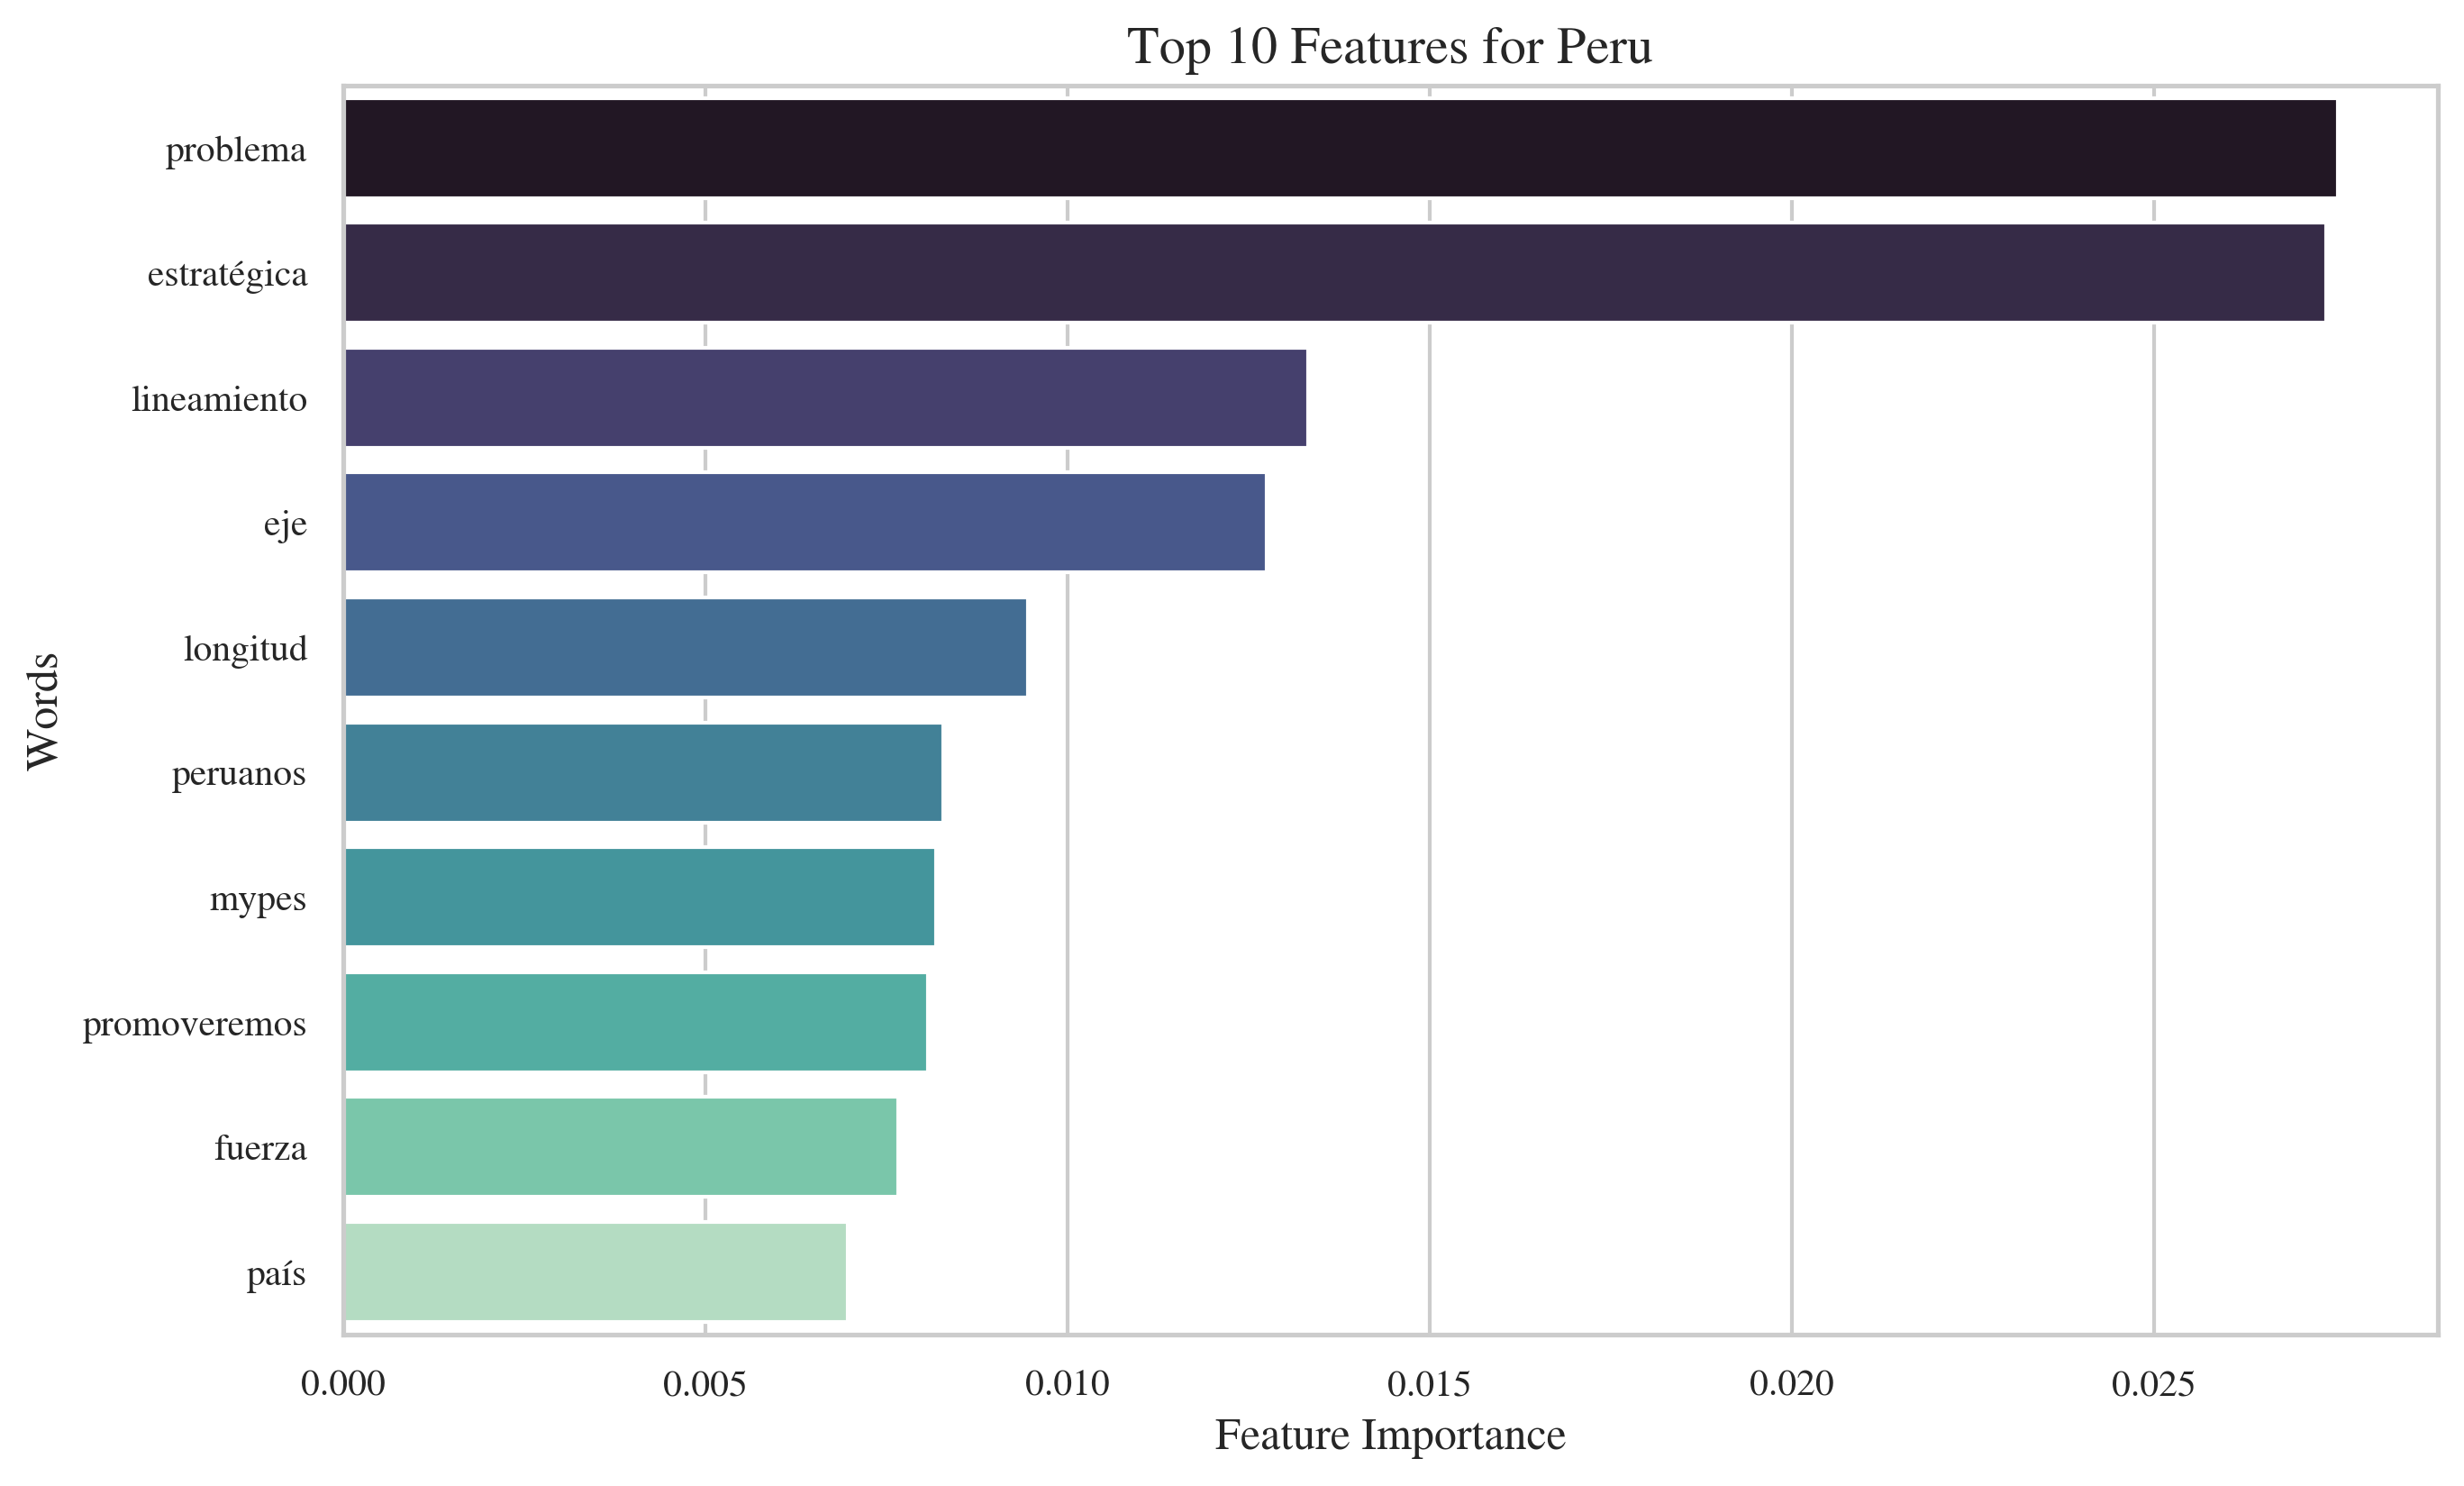
\includegraphics[width=0.8\textwidth]{/Users/sarabcidf/Desktop/ASDS/Dissertation/FinalScripts/CallanByCountry/Peru_feature_importance.png}
	\end{figure}
	\begin{figure}[H]
		\centering
		\caption{Error Rate for Peru Model}
		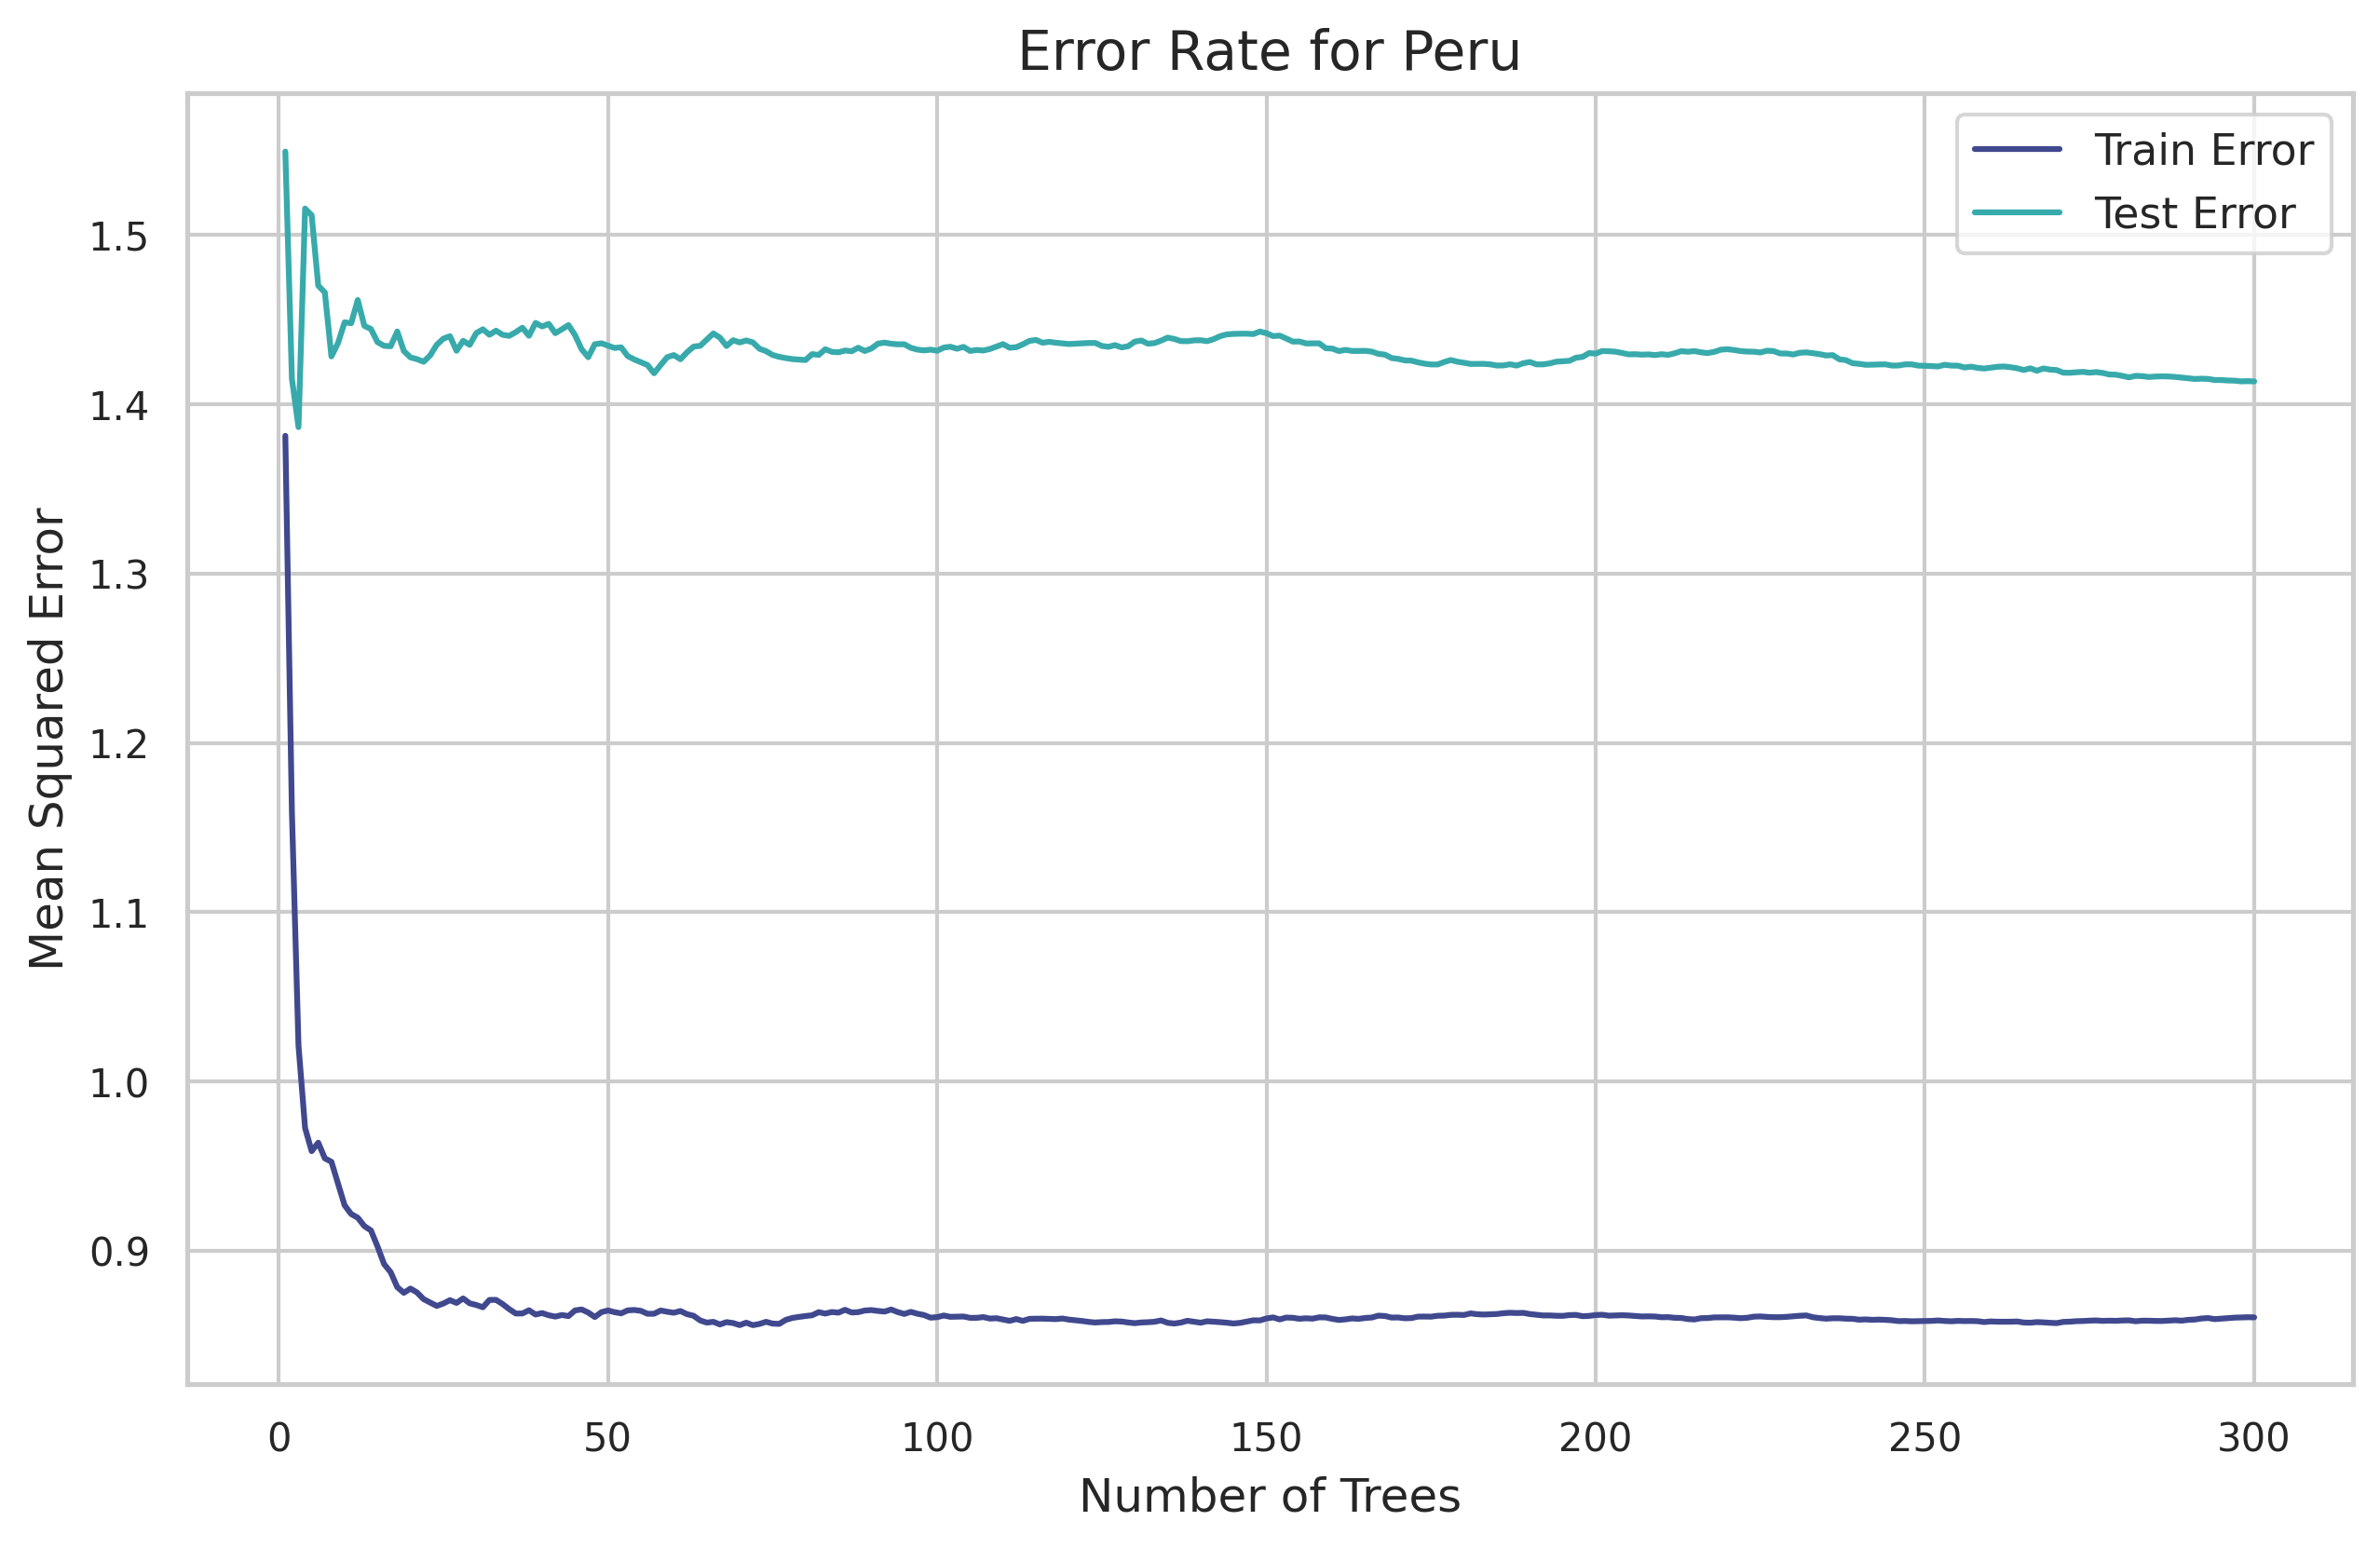
\includegraphics[width=0.8\textwidth]{/Users/sarabcidf/Desktop/ASDS/Dissertation/FinalScripts/CallanByCountry/Peru_error_rate.png}
	\end{figure}
	\begin{figure}[H]
		\centering
		\caption{Learning Curve for Peru Model}
		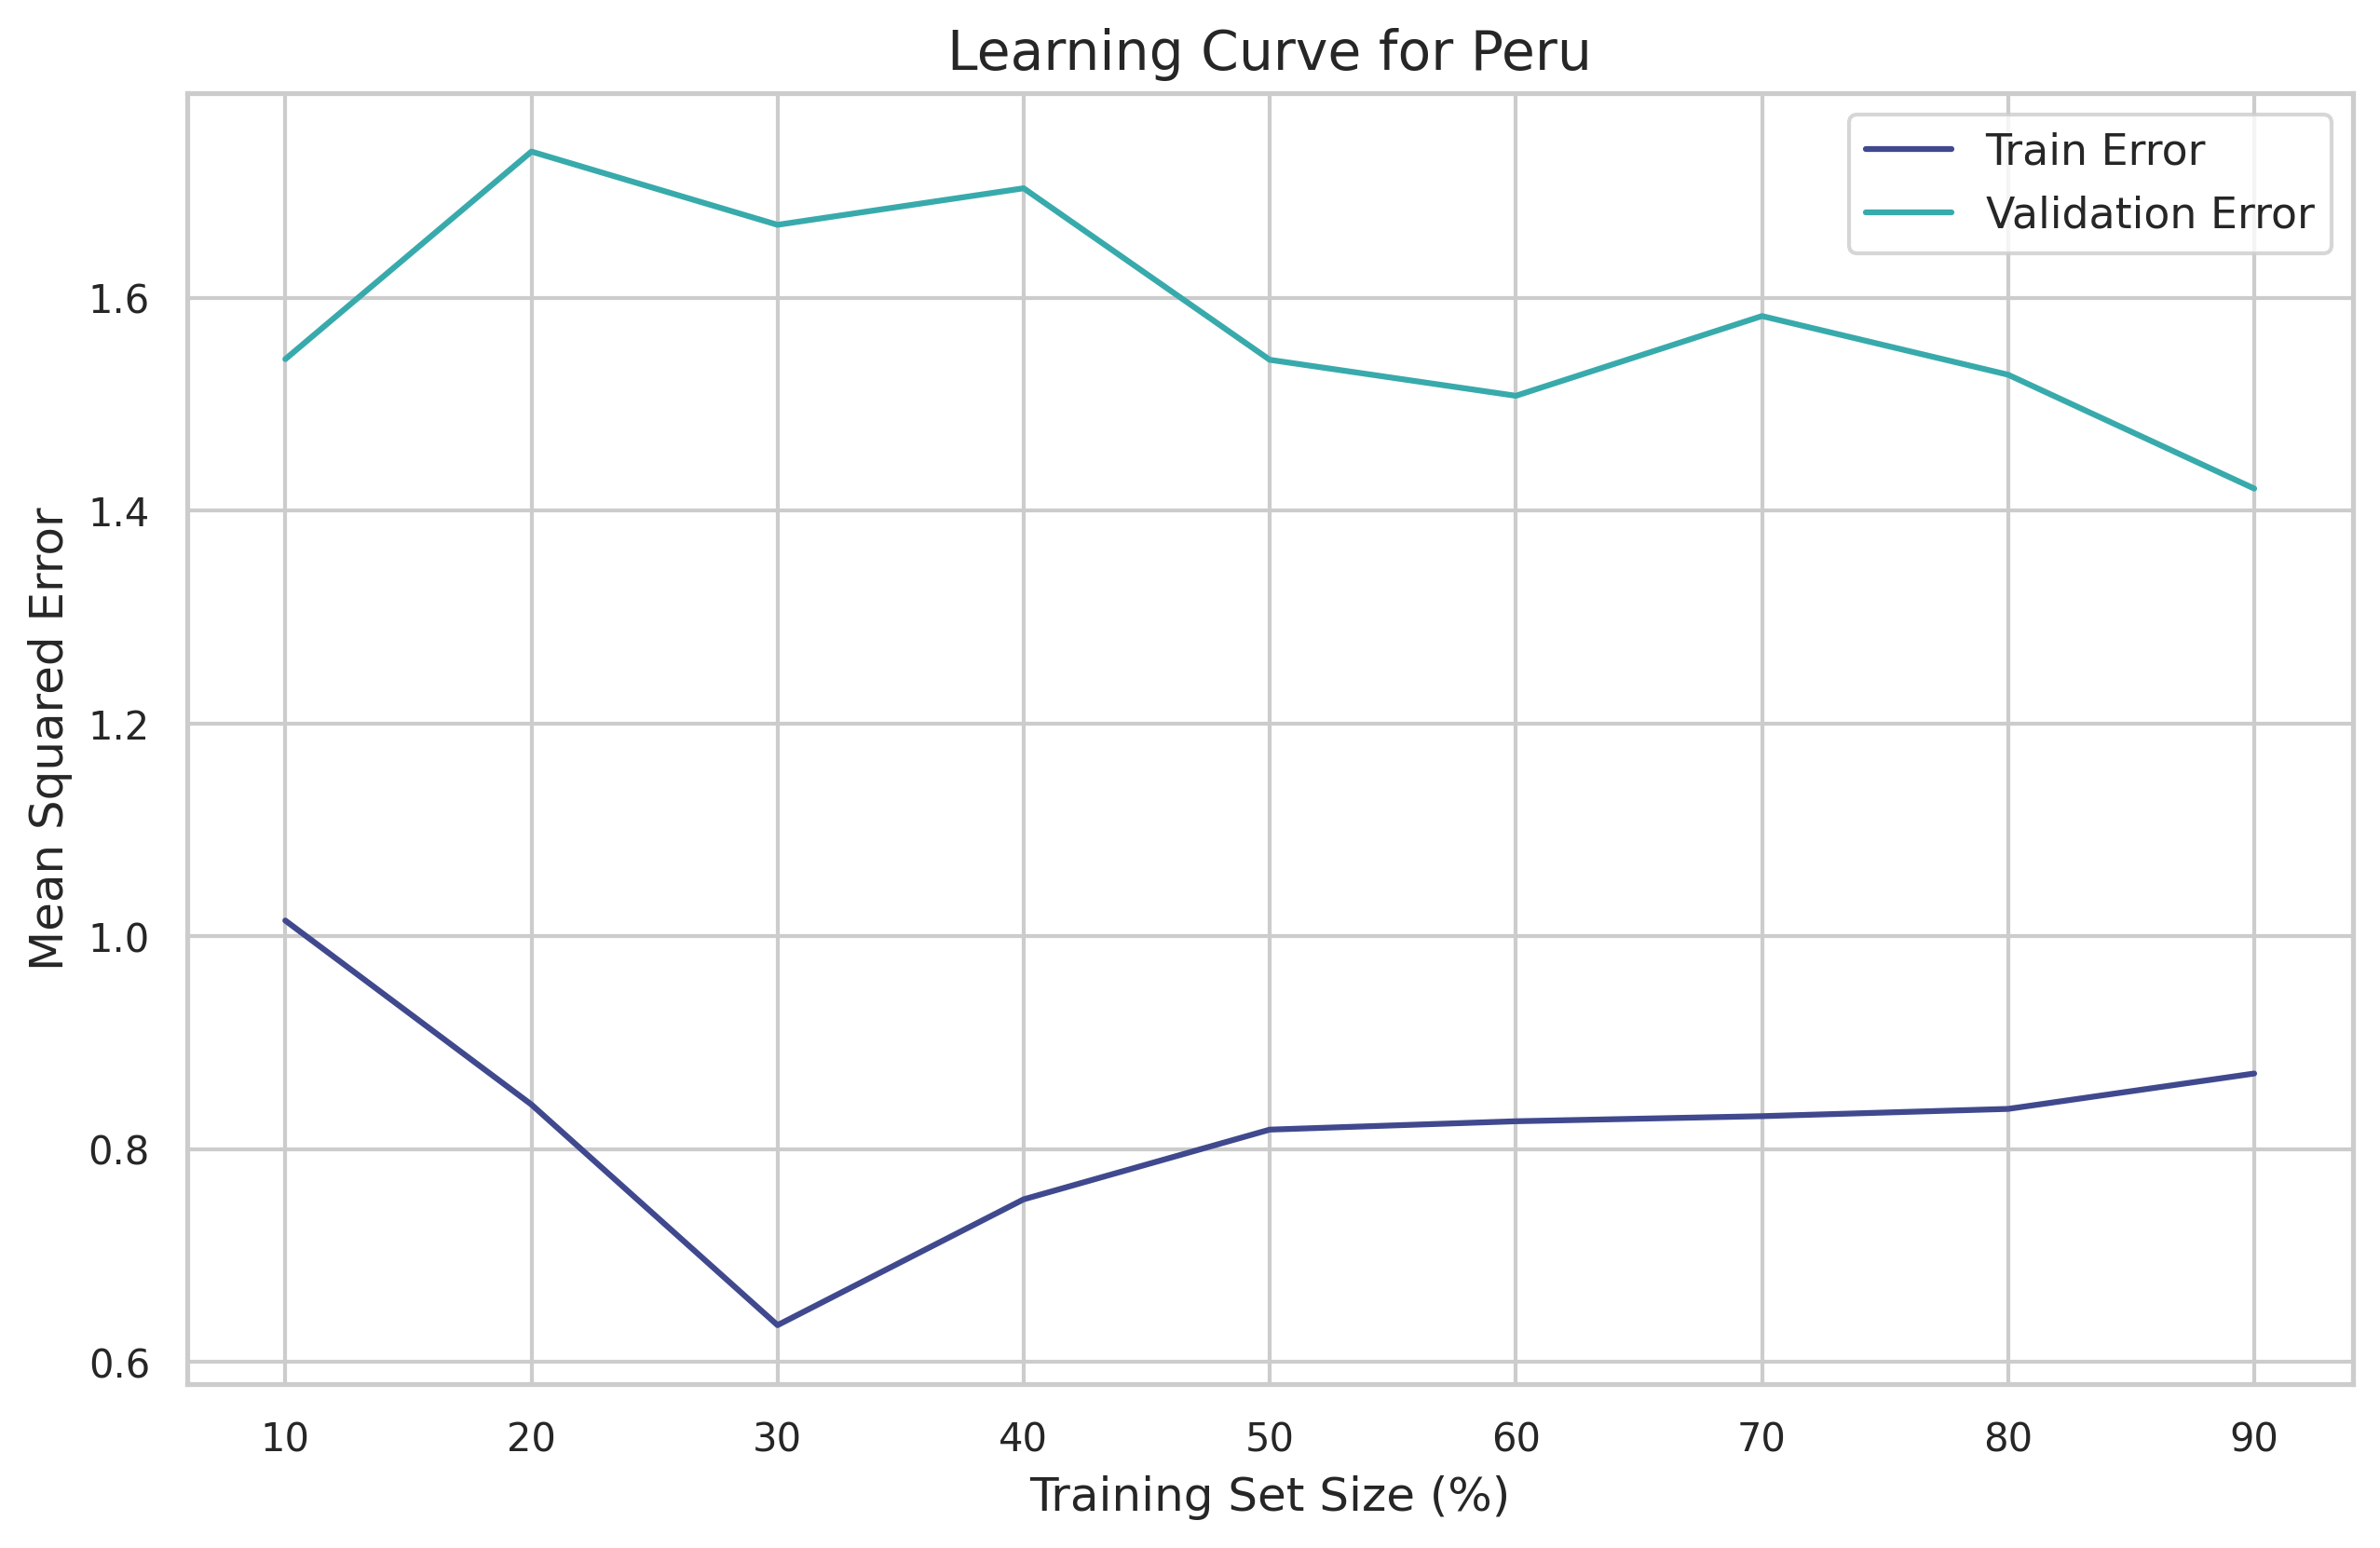
\includegraphics[width=0.8\textwidth]{/Users/sarabcidf/Desktop/ASDS/Dissertation/FinalScripts/CallanByCountry/Peru_learning_curve.png}
	\end{figure}
	
	\newpage
	
	\subsection{Uruguay}
	\begin{figure}[H]
		\centering
		\caption{Feature Importance for Uruguay Model}
		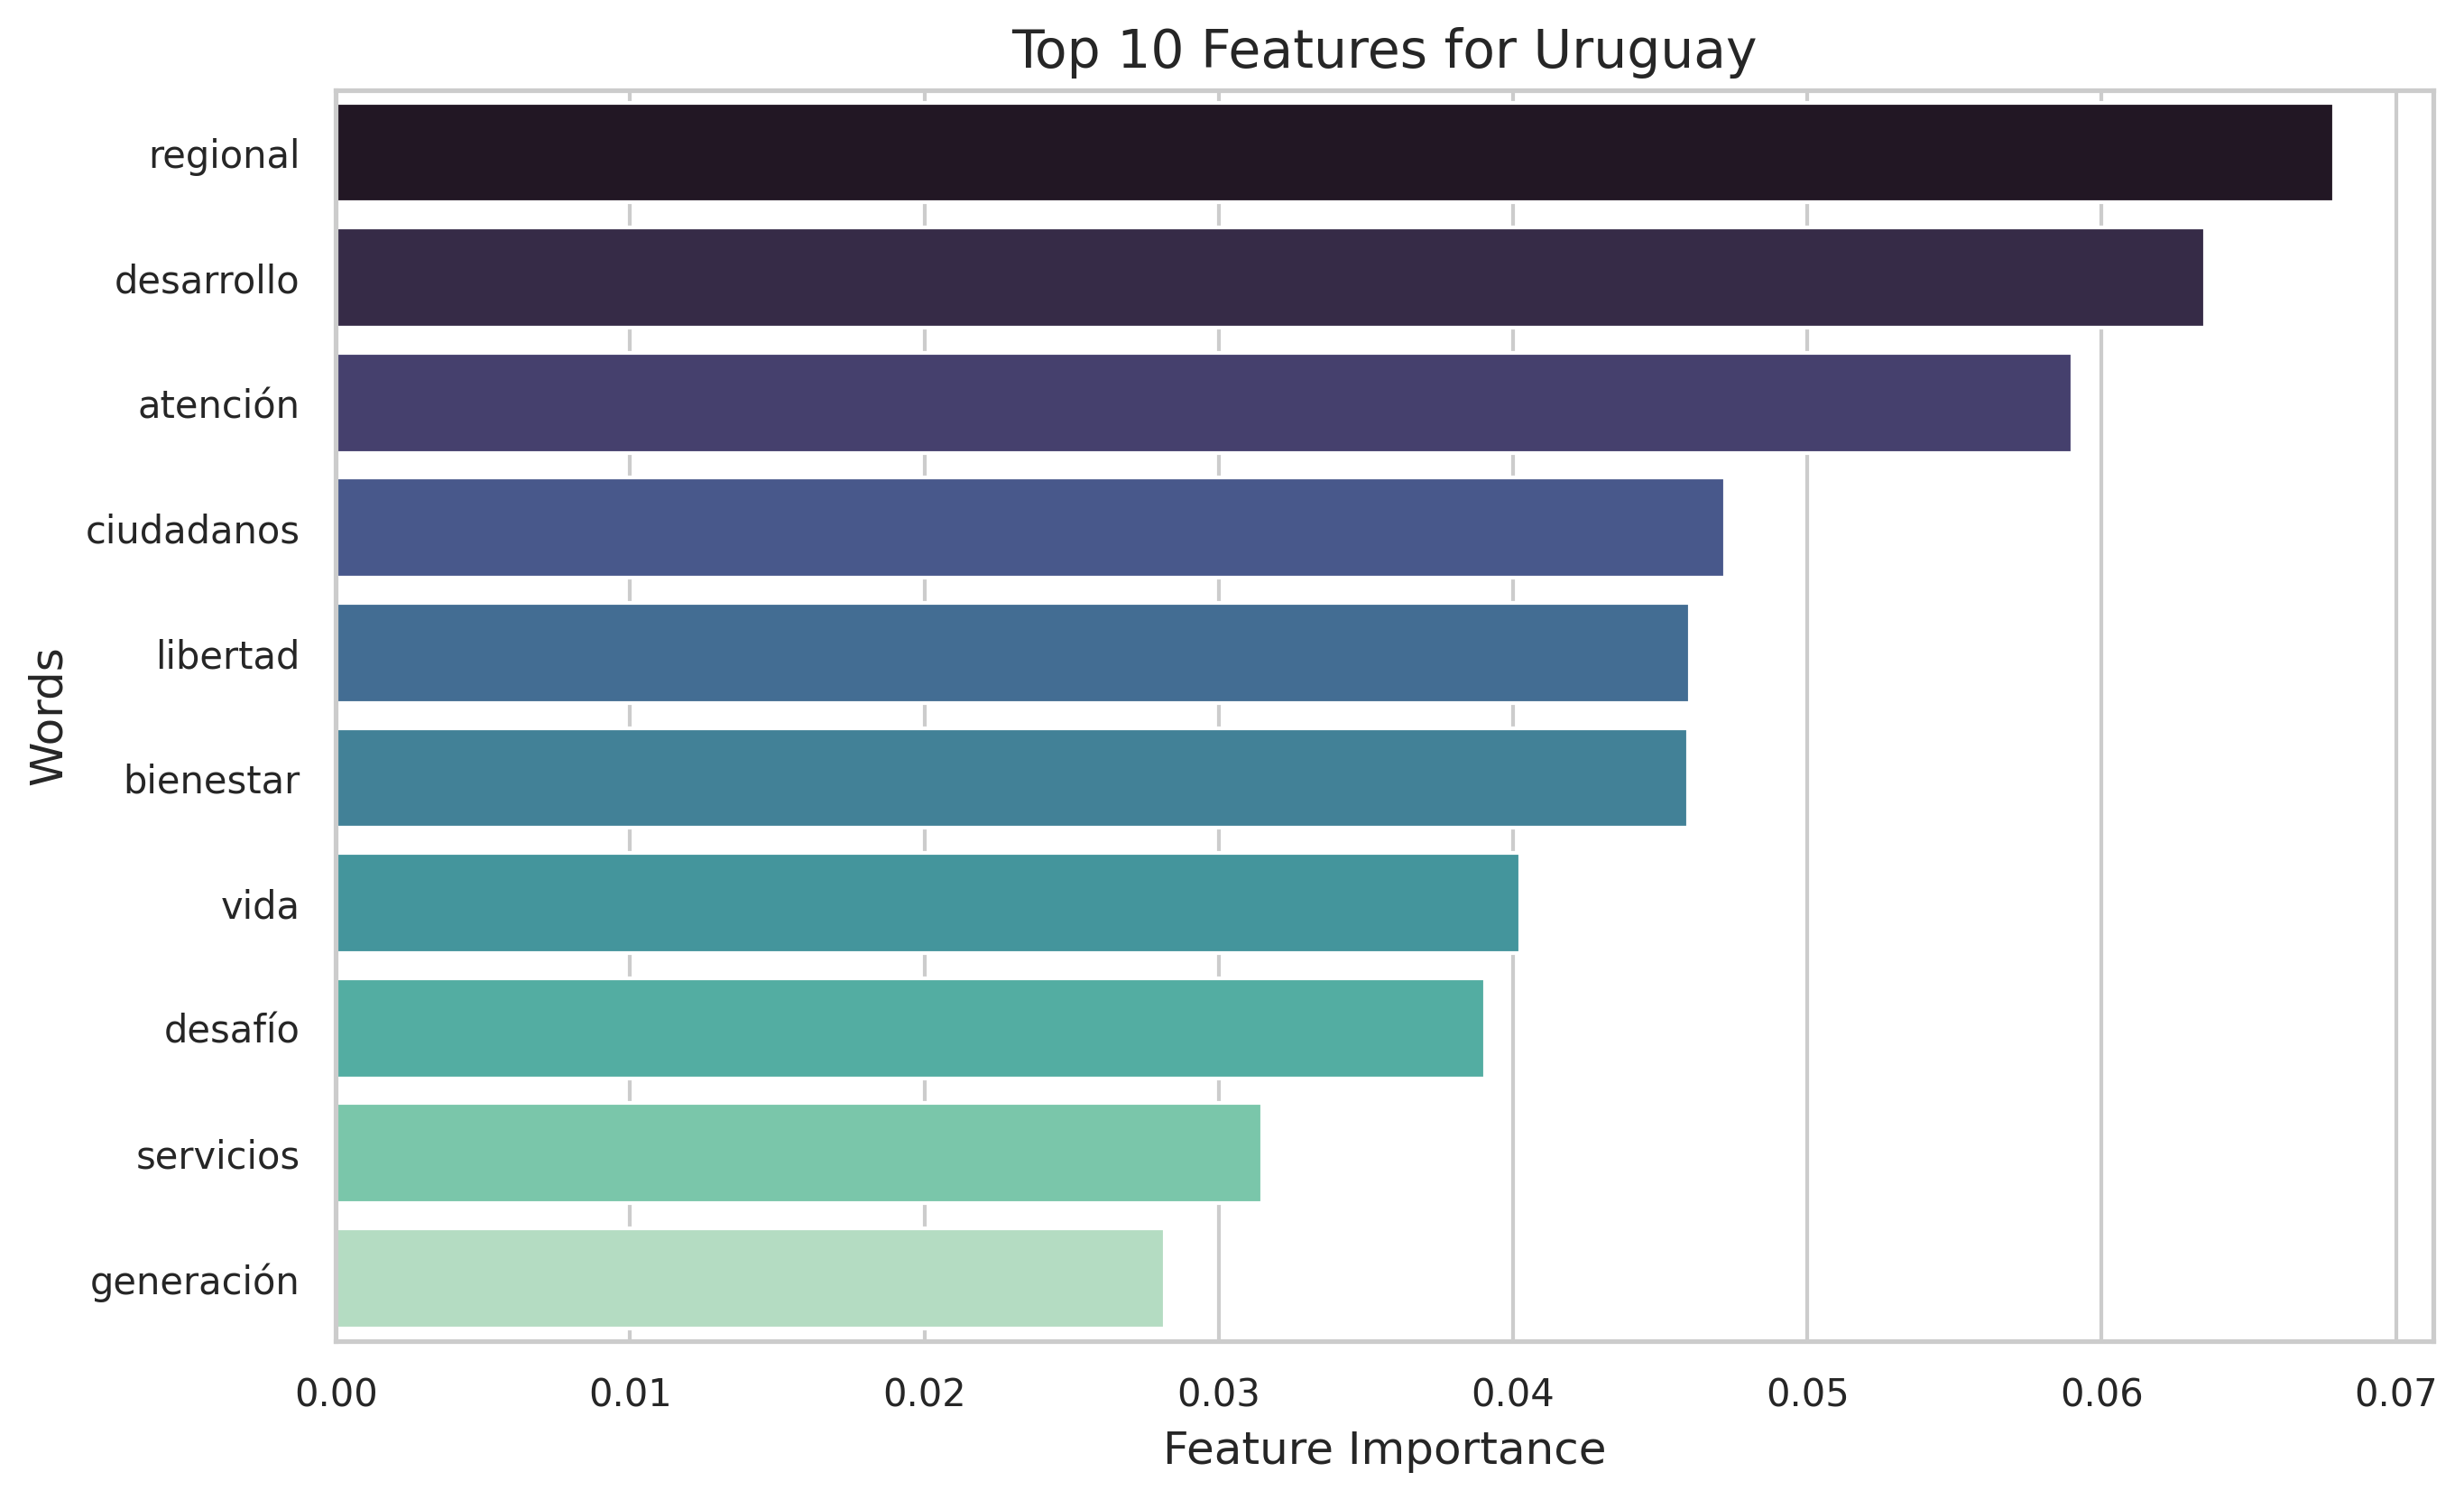
\includegraphics[width=0.8\textwidth]{/Users/sarabcidf/Desktop/ASDS/Dissertation/FinalScripts/CallanByCountry/Uruguay_feature_importance.png}
	\end{figure}
	\begin{figure}[H]
		\centering
		\caption{Error Rate for Uruguay Model}
		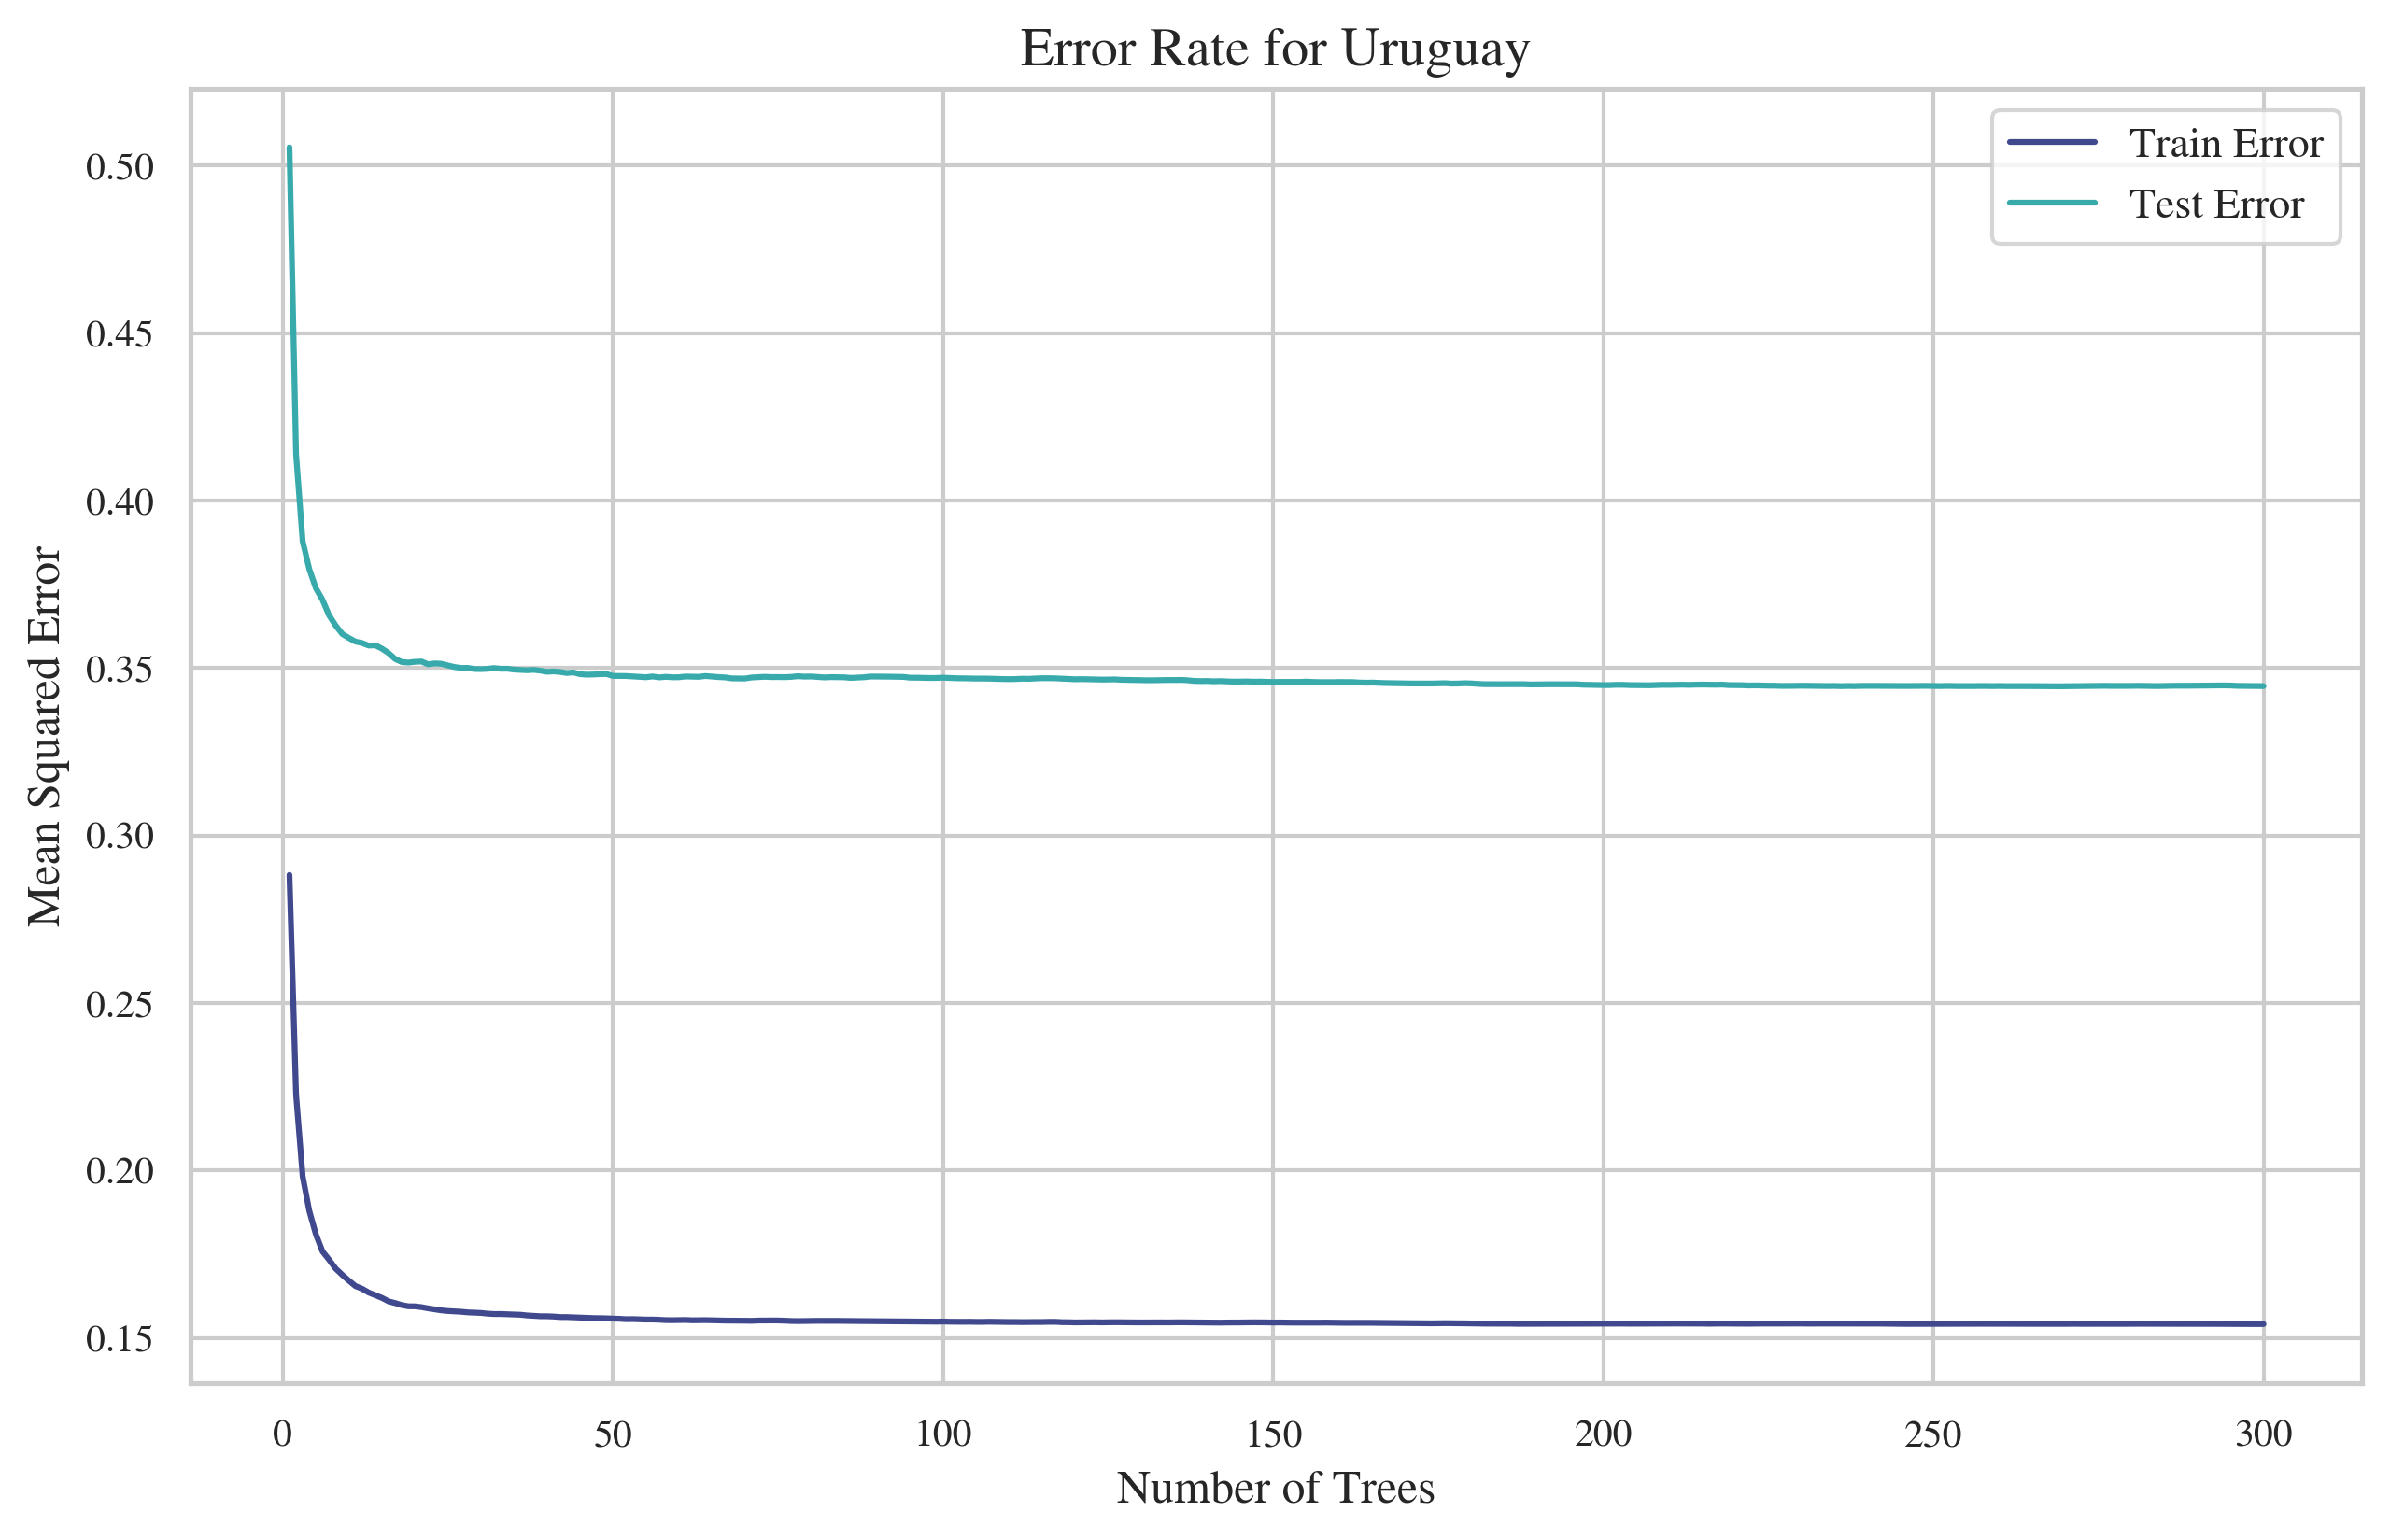
\includegraphics[width=0.8\textwidth]{/Users/sarabcidf/Desktop/ASDS/Dissertation/FinalScripts/CallanByCountry/Uruguay_error_rate.png}
	\end{figure}
	\begin{figure}[H]
		\centering
		\caption{Learning Curve for Uruguay Model}
		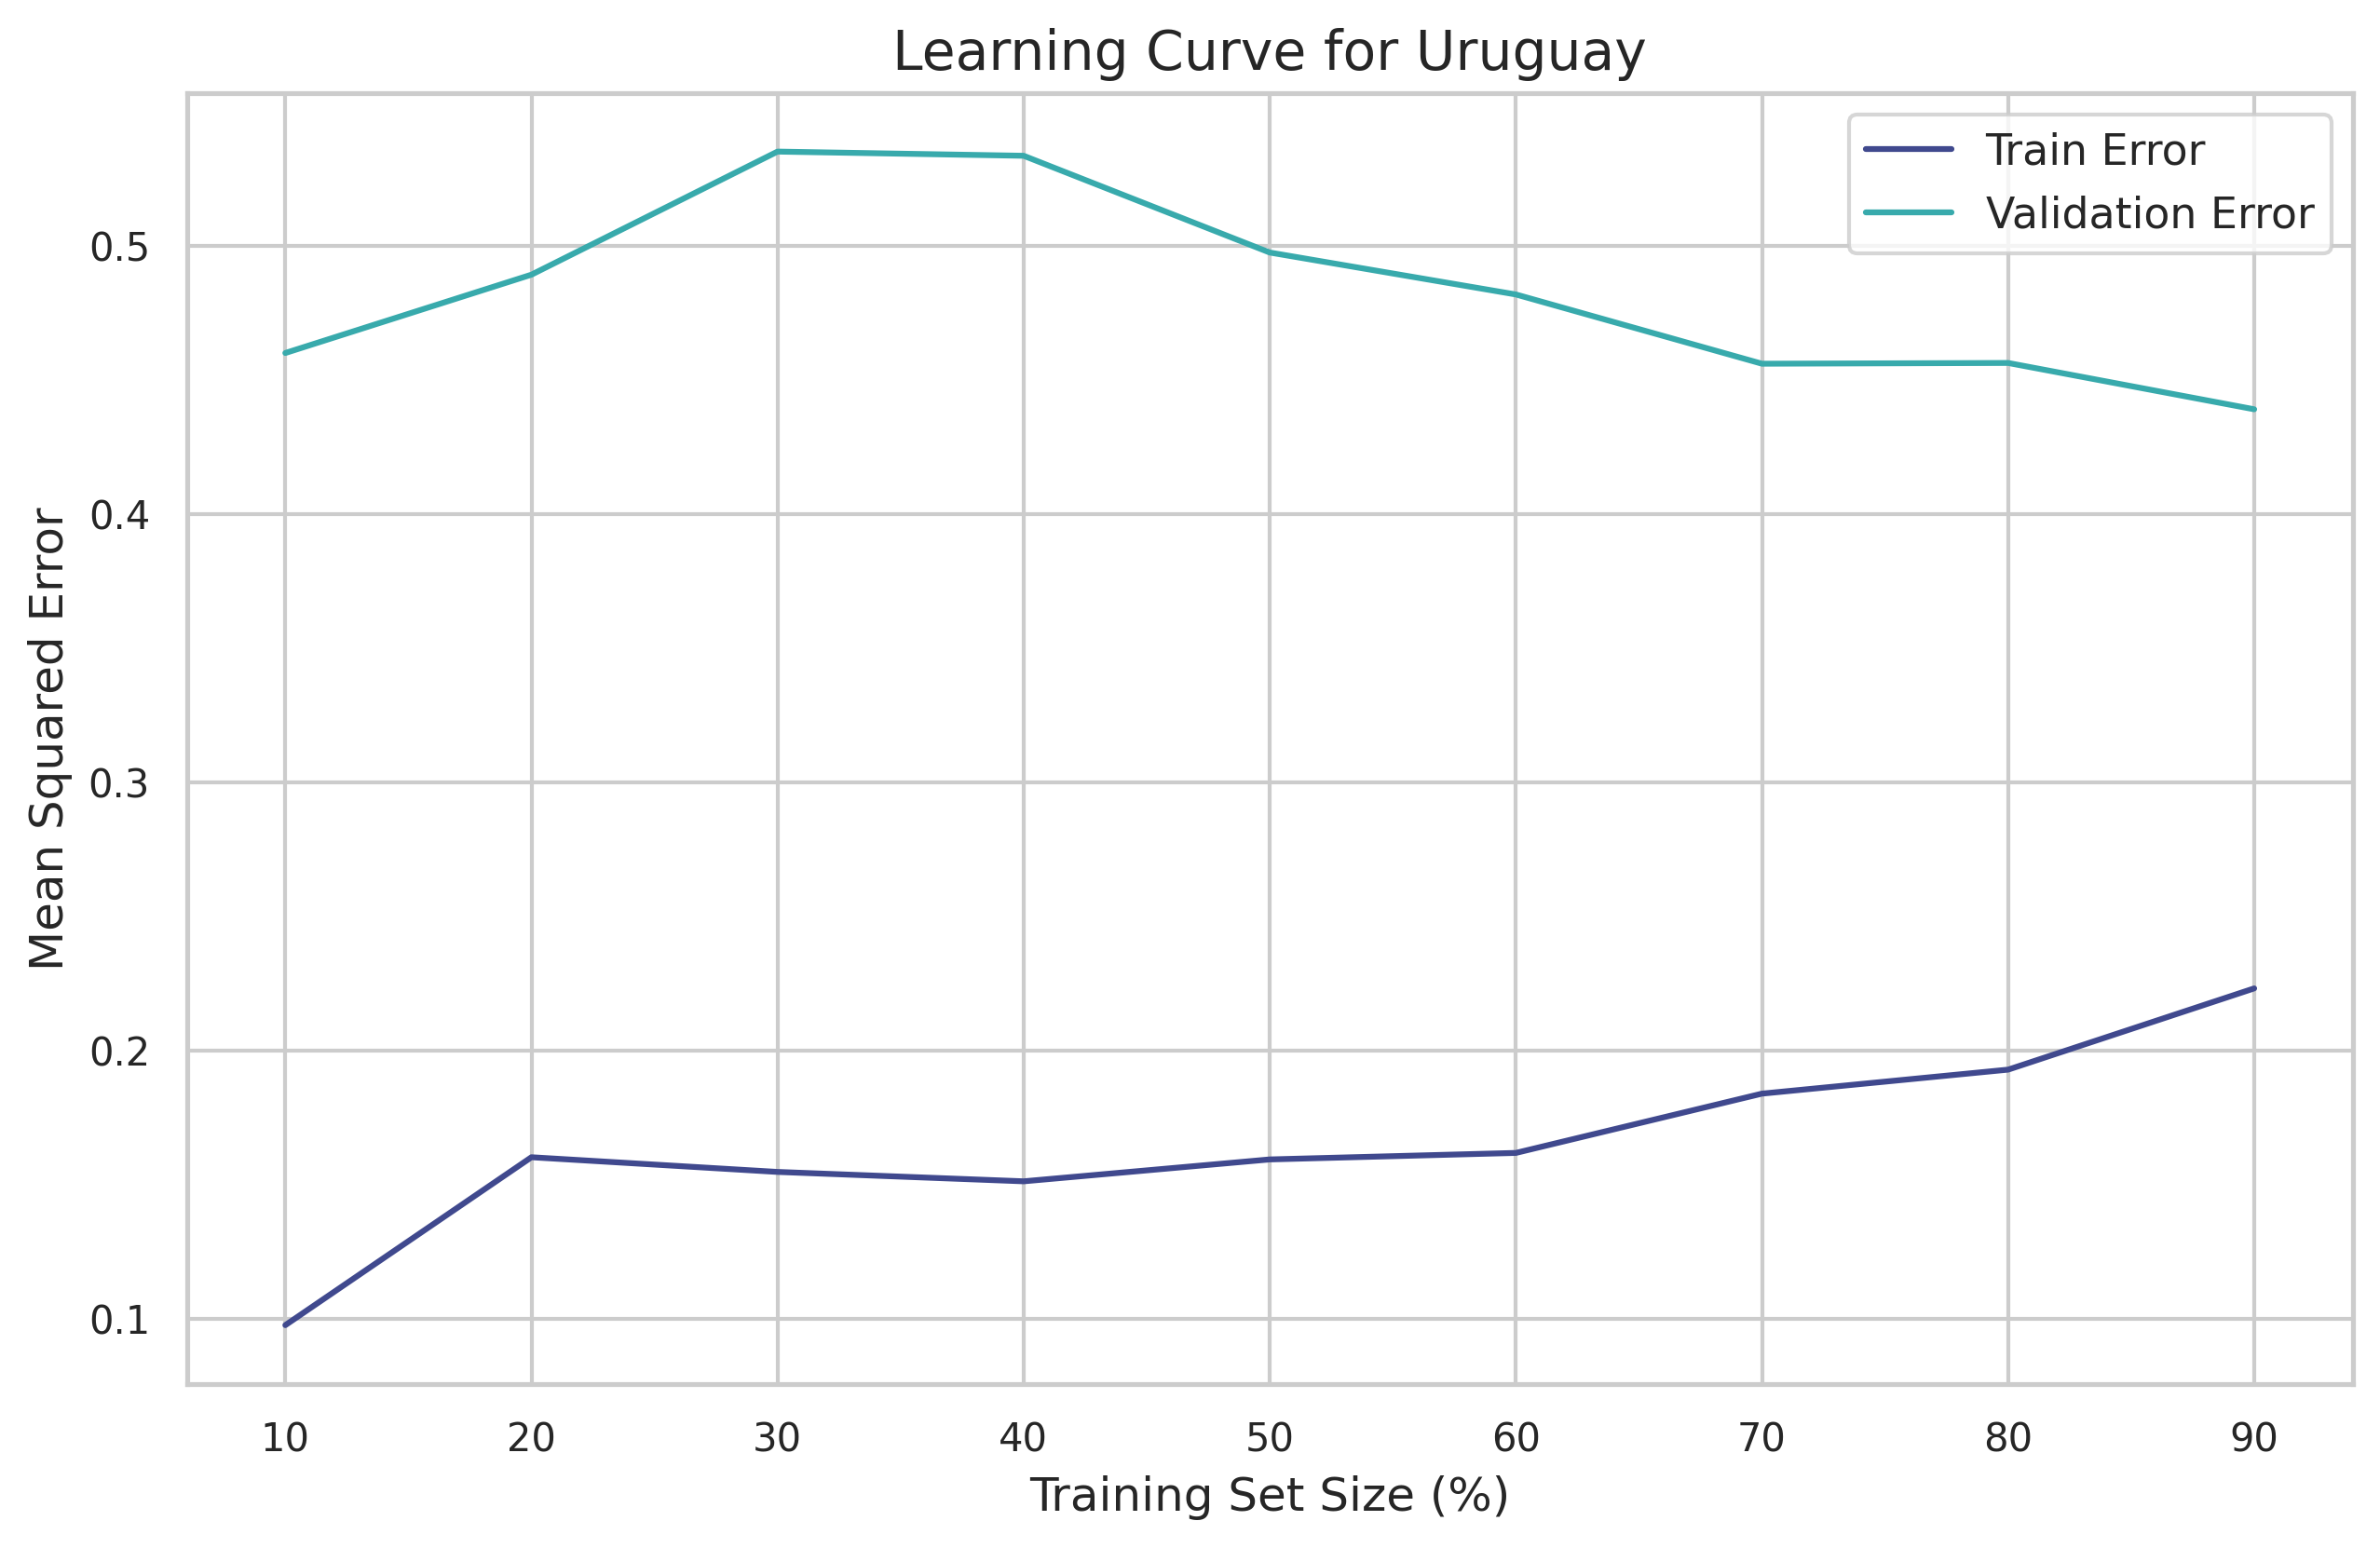
\includegraphics[width=0.8\textwidth]{/Users/sarabcidf/Desktop/ASDS/Dissertation/FinalScripts/CallanByCountry/Uruguay_learning_curve.png}
	\end{figure}
	
	\subsection{Predictions by party (all parties)}
	
	\begin{longtable}{|>{\centering\arraybackslash}m{7cm}|>{\centering\arraybackslash}m{3cm}|>{\centering\arraybackslash}m{3cm}|}
		\caption{Party Name, Country, and Scaled Prediction} \\
		\hline
		\textbf{Party Name} & \textbf{Country} & \textbf{Scaled Prediction} \\ \hline
		\endfirsthead
		\hline
		\textbf{Party Name} & \textbf{Country} & \textbf{Scaled Prediction} \\ \hline
		\endhead
		\hline
		\endfoot
		\hline
		\endlastfoot
		Dominican Liberation Party & D. Republic & 8.20 \\ \hline
		Modern Revolutionary Party & D. Republic & 8.02 \\ \hline
		Movement towards Socialism - Political Instrument for the Sovereignty of the Peoples & Bolivia & 7.27 \\ \hline
		Proud and Sovereign Fatherland Alliance Movement & Ecuador & 6.98 \\ \hline
		Patriotic Society Party & Ecuador & 6.94 \\ \hline
		Social Christian Party & Ecuador & 6.88 \\ \hline
		Christian Democratic Party & Bolivia & 6.85 \\ \hline
		Democratic Left & Ecuador & 6.36 \\ \hline
		People’s Force & Peru & 6.28 \\ \hline
		Creating Opportunities & Ecuador & 6.19 \\ \hline
		Democratic Change & Panama & 6.12 \\ \hline
		Labor Party & Mexico & 6.11 \\ \hline
		Force 2011 & Peru & 6.05 \\ \hline
		Democratic Revolutionary Party & Panama & 5.84 \\ \hline
		National Solidarity Alliance & Peru & 5.65 \\ \hline
		Alliance for Progress of Peru & Peru & 5.62 \\ \hline
		Alliance for the Great Change & Peru & 5.59 \\ \hline
		New Majority for Chile & Chile & 5.56 \\ \hline
		Approve Dignity & Chile & 5.56 \\ \hline
		New Social Pact & Chile & 5.56 \\ \hline
		Broad Front & Chile & 5.56 \\ \hline
		Alliance Possible Peru & Peru & 5.56 \\ \hline
		Christian Social Front & Chile & 5.55 \\ \hline
		Colombian Conservative Party & Colombia & 5.39 \\ \hline
		Party of Radical Change & Colombia & 5.38 \\ \hline
		Popular Action & Peru & 5.36 \\ \hline
		Party of U & Colombia & 5.36 \\ \hline
		Alternative Democratic Pole & Colombia & 5.26 \\ \hline
		Green Alliance & Colombia & 5.24 \\ \hline
		Peruvians for Change & Peru & 5.24 \\ \hline
		Popular Alliance & Peru & 5.19 \\ \hline
		Green Party & Colombia & 5.18 \\ \hline
		National Regeneration Movement & Mexico & 5.18 \\ \hline
		Independent & Panama & 5.13 \\ \hline
		Colombian Liberal Party & Colombia & 5.11 \\ \hline
		Libertarian Movement Party & Costa Rica & 4.71 \\ \hline
		National Restoration Party & Costa Rica & 4.68 \\ \hline
		Progressive Movement & Mexico & 4.51 \\ \hline
		National Integration Party & Costa Rica & 4.50 \\ \hline
		Social Christian Republican Party & Costa Rica & 4.39 \\ \hline
		Democratic Revolutionary Party & Mexico & 4.34 \\ \hline
		Social Encounter Party & Mexico & 4.33 \\ \hline
		Coalition ‘We save Mexico' & Mexico & 4.31 \\ \hline
		Convergence & Mexico & 4.29 \\ \hline
		Convergence for Democracy & Mexico & 4.27 \\ \hline
		Coalition ‘Mexico First' & Mexico & 4.25 \\ \hline
		New Alliance Party & Mexico & 4.22 \\ \hline
		Commitment for Mexico & Mexico & 4.21 \\ \hline
		Social Christian Unity Party & Costa Rica & 4.20 \\ \hline
		Alliance for Mexico 2006 & Mexico & 4.18 \\ \hline
		Citizens' Movement & Mexico & 4.04 \\ \hline
		Alliance for Change & Mexico & 3.91 \\ \hline
		National Liberation Party & Costa Rica & 3.90 \\ \hline
		Broad Front & Costa Rica & 3.67 \\ \hline
		Citizen’s Action Party & Costa Rica & 3.50 \\ \hline
		Broad Front & Uruguay & 2.52 \\ \hline
		Colorado Party & Uruguay & 2.31 \\ \hline
		National Party & Uruguay & 2.27 \\ \hline
		Independent Party & Uruguay & 2.14 \\ \hline
	\end{longtable}
	
\end{document}

